%\documentclass[11pt]{article}
%\usepackage[a4paper,margin=1in]{geometry}
%\usepackage{amsmath,amssymb}
%\usepackage{booktabs}
%\usepackage{array}
%\usepackage[T1]{fontenc}
%\usepackage{lmodern}
%\usepackage{microtype}
%
%\title{Nonnegative Matrix Factorization for Transcriptomics}
%\author{}
%\date{}

% A Master's-Level Introduction to D-SPIN
% Expanded educational version
%
% Based on:
% J. Jiang et al., "D-SPIN constructs regulatory network models from
% scRNA-seq revealing organizing principles of perturbation response",
% Cell 189 (2026), 4159--4184.e35.	
%
% This document is an educational simplification of the published method.
% It intentionally omits some computational and inferential details.

\documentclass[11pt,a4paper]{article}

\usepackage[margin=2.5cm]{geometry}
\usepackage{amsmath,amssymb,bm,mathtools}
\usepackage{booktabs}
\usepackage{hyperref}
\usepackage{enumitem}
\usepackage{microtype}
\usepackage{setspace}
\usepackage{titlesec}
\usepackage{parskip}
\usepackage{graphicx}
\usepackage{xcolor}
\usepackage{ulem}
\usepackage{tikz}
\usepackage{relsize}
\usetikzlibrary{positioning}

\setstretch{1.08}
\setlength{\parindent}{0pt}
\setlength{\parskip}{0.55em}

\titleformat{\section}
{\Large\bfseries}
{\thesection}
{0.7em}
{}
\titleformat{\subsection}
{\large\bfseries}
{\thesubsection}
{0.7em}
{}
\titleformat{\subsubsection}
{\normalsize\bfseries}
{\thesubsubsection}
{0.7em}
{}

\newcommand\identity{1\kern-0.25em\text{l}}

\definecolor{darkgreen}{RGB}{0,80,0}
\definecolor{darkred}{RGB}{110,0,0}
\definecolor{darkishgreen}{RGB}{34,139,84}
\definecolor{darkishred}{RGB}{180,70,70}
\newcommand{\enrichedbox}{%
	\makebox[0.65cm][l]{\textcolor{darkishgreen}{\rule{0.18cm}{0.18cm}}}%
}
\newcommand{\notenrichedbox}{%
	\makebox[0.65cm][l]{\textcolor{darkishred}{\rule{0.18cm}{0.18cm}}}%
}

%\hypersetup{
%\noindent     colorlinks=true,
%\noindent     linkcolor=blue,
%\noindent     citecolor=blue,
%\noindent     urlcolor=blue
%\noindent }

%\title{Nonnegative Matrix Factorization for Transcriptomics}
\title{From NMF to D-SPIN}
\author{A nonnecessary master thesis by Demetrio Magatti}
\date{\today}

\begin{document}

\thispagestyle{empty}
\maketitle
\thispagestyle{empty}
\clearpage
\thispagestyle{empty}

\newpage

\thispagestyle{empty}
\tableofcontents
\clearpage

\pagenumbering{arabic}

\newpage

\section{Nonnegative Matrix Factorization for transcriptomics}

%This section is based on the \textit{Learning the parts of objects by nonnegative matrix factorization} paper by D. D. Lee and H. S. Seung, expanded to cover genomics-related applications. The goal here so to extract and highlight the key points, while avoiding deep-diving into optimization algorithms, loss functions to be minimized and so on. The original paper is obviously much more detailed when it comes to that.

\subsection{Image-related NMF}

Let's take a collection of black-and-white images containing faces. Each picture contains a total on $n$ pixels.

Each image can be flattened from 2 dimensions to 1 by collapsing it into a vector of $n$ pixel intensities. Given $m$ images, the result of the flattening is a matrix of positive values (pixel intensities cannot be negative)

\[
Y \in \mathbb{R}_{\geq 0}^{n\times m}
\]

The image database \textit{Y} is regarded as an $n \times m$ matrix V, each column of which contains \textit{n} nonnegative pixel
values of one of the \textit{m} facial images. 

The goal of \textbf{Nonnegative Matrix Factorization} (\textbf{NMF}) is to decompose \textit{Y} in a structure like 

\[
Y \approx HW
\]

or, more explicitly,

\[ 
Y_{i \mu} \approx \sum_{\alpha = 1}^r W_{i \alpha} H_{\alpha \mu}
\]

while imposing the \textbf{nonnegativity constraint}

\[
H\in\mathbb{R}_{\geq0}^{n\times r}
\qquad
W\in\mathbb{R}_{\geq0}^{r\times m}
\]

The columns of \textit{W} are called basis images. Each column of \textit{H} is called an encoding, and is in one-to-one
correspondence with a face in \textit{Y} . An encoding consists of the coefficients by which a face is represented with
a linear combination of basis images. Conceptually, NMF is not fundamentally different from other dimensionality-reduction techniques such as PCA: its goal is to extract a set of latent “features” that can be combined to provide a faithful reconstruction of the original data. The key difference is the nonnegativity constraint, which restricts the reconstruction to additive combinations of these features.

\begin{figure}[h]
	\centering
	\setlength{\abovecaptionskip}{2pt}
	\[
	\begin{array}{c@{\qquad}c}
	\begin{array}{c}
	\textbf{PCA}\\[4pt]
	X\approx
	\underset{H}{
		\begin{array}{|cc|}
		\hline
		+&-\\
		+&+\\
		-&+\\
		-&-\\
		\hline
		\end{array}}
	\;
	\underset{W}{
		\begin{array}{|cccc|}
		\hline
		+&+&-&-\\
		-&+&+&-\\
		\hline
		\end{array}}
	\\[8pt]
	%\downarrow\\[-2pt]
	\\[-8pt]
	\text{signed directions}\\
	\text{addition or subtraction allowed}
	\end{array}
	&
	\qquad \qquad
	\begin{array}{c}
	\textbf{NMF}\\[4pt]
	X\approx
	\underset{H}{
		\begin{array}{|cc|}
		\hline
		+&0\\
		+&+\\
		0&+\\
		0&+\\
		\hline
		\end{array}}
	\;
	\underset{W}{
		\begin{array}{|cccc|}
		\hline
		+&+&+&0\\
		+&0&0&+\\
		\hline
		\end{array}}
	\\[8pt]
	%\downarrow\\[-2pt]
	\\[-8pt]
	\text{non-negative parts}\\
	\text{additive only}
	\end{array}
	\end{array}
	\]
	\caption{Comparison of PCA and non-negative matrix factorization (NMF).}
	\label{fig:pca_vs_nmf_schematic}
\end{figure}

The nonnegativity constraint plays a central role in determining the type of representation learned by NMF. Since both the basis images and their coefficients are nonnegative, the original image can only be reconstructed by adding the learned components together. This encourages each component to capture distinct, localized structures that can be combined to reconstruct the whole image, leading naturally to a part-based representation. Unlike methods that allow positive and negative contributions to cancel each other, NMF therefore tends to learn features corresponding to meaningful image parts.

%The nonnegativity constraint plays a central role in determining the type of representation learned by NMF. Since both the basis images and their coefficients are constrained to be nonnegative, the original image can only be reconstructed by adding the learned components together. In this setting, each component can capture a distinct part of the image, and different parts can be combined to reconstruct the whole. This leads naturally to the intuitive notion of combining parts to form a whole, which is how NMF learns a part-based representation. Learned features correspond to meaningful and localized structures rather than to combinations involving both positive and negative contributions.

%This nonnegativity constraint is what makes NMF different from ohter dimensionality reduction techniques like Principal Component Analysis. These constraints permit the combination of multiple basis images to represent a face, with the key point of only allowing additive combinations. In contrast to PCA, no subtractions can occur. For these reasons, the nonnegativity constraints are compatible with the intuitive notion of combining parts to form a whole, which is how NMF learns a part-based representation.

\textcolor{red}{Add citation somewhwere.}



\begin{figure}[h]
	\centering
	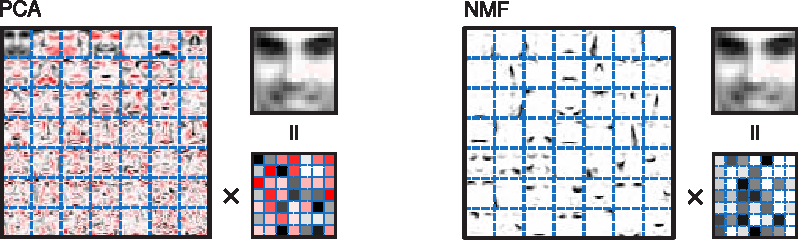
\includegraphics[width=0.9\textwidth]{img/PCA_NMF.pdf}
	\caption{Image decomposition. PCA constructs a set of \textit{eigenfaces}, while NMF favours a parts-based representation}.
	\label{fig:pca_vs_nmf_faces}
\end{figure}

\subsection{Bridging to genomics}

Additive-only combinations are quite interesting when it comes to genomics, as a "negative" expression of a gene is something that cannot happen in nature and it is of difficult interpretation and understanding. 

Therefore, we aim to build a correspondence which looks something like this

\begin{center}
\begin{tabular}{ll}
\toprule
Image NMF & Transcriptomics \\
\midrule
\textbf{source image} & \textbf{sample / spatial location} \\
\textbf{pixels} & \textbf{genes} \\
\textbf{basis image} & \textbf{gene-expression program / factor} \\
\textbf{encoding of an image} & \textbf{factor activity in a sample/location} \\
\bottomrule
\end{tabular}
\end{center} 
\vspace{2mm}
We can think of \textbf{gene program} as set or pattern of genes whose expression tends to vary together and that collectively reflects a biological process, cell state, or cellular function. In the specific context of NMF, the term usually refers more specifically to a learned factor characterized by a group of genes with high nonnegative weights, rather than to a predefined gene set. 

\subsubsection{Source images}

In image decomposition, you start with an image such as

\[
\boxed{\text{one image} = \text{one observation}}
\]

Each row of your matrix is one face, i.e. a set of pixel intensities which is unique to a specific face

\[
Y_i =
[\text{pixel}_1,\text{pixel}_2,\ldots,\text{pixel}_{n}].
\]

In ordinary transcriptomics, we can make exactly the same construction. Suppose you have \textit{m} cells and measure \textit{n} genes. We go back exaclty to 

\[
Y\in\mathbb{R}_{\geq0}^{n\times m}.
\]

but now each row is now one cell

\[
Y_i =
[\text{gene}_1,\text{gene}_2,\ldots,\text{gene}_{n}].
\]

The explicit analogy is

\[
\boxed{
\text{image}
\longleftrightarrow
\text{cell/sample}
}
\]

The image is a single observation whose features are pixel intensities.

The cell is a single observation whose features are gene-expression counts.

\subsubsection{Pixels}

images have pixel intensities

\[
[\text{pixel}_1,~\text{pixel}_2,~\ldots,~\text{pixel}_{n}]
\]

whereas a genomic sample has 

\[
[\text{gene}_1,~\text{gene}_2,~\ldots,~\text{gene}_{n}].
\]

so the most direct analogy is

\[
\boxed{
	\text{pixel}
	\longleftrightarrow
	\text{gene expression}
}
\]

In both cases, these are the \textbf{features} describing the observation.

There is a key difference to be noted. Pixels have a very obvious spatial relationship (e.g. pixel 100 is physically next to pixel 101), while genes generally don't have such a geometric relationship. Gene 100 is not necessarily ``close'' to gene 101 in any meaningful sense. When dealing with tissue samples where gene location is available, spatial information can be used. The process is an extension of NMF known as Nonnegative Spatial Factorization (NSF).

\subsubsection{Basis images}

Say that, for example, NMF discovers $r=10$ basis images. For $j = 1, ..., r$ we get 

\[
W_1 =
\begin{bmatrix}
w^j_1, \ldots , w^j_n
\end{bmatrix}
\]

Each $W_j$ corresponds to a specific part of the faces: $W_1$ looks like an eye, $W_2$ looks like a nose, and so on. The key point is that a basis image is \textbf{not itself one of your original images}.

It is a learned pattern that can be used to reconstruct the original images. For one specific source image

\[
\text{face}
\approx
2.0(\text{eyes})
+
0.8(\text{nose})
+
1.3(\text{mouth})
\]

The numbers $2.0,0.8,1.3$ are the \textbf{encoding} for that particular face.

For transcriptomics, we replace ``pixel intensity'' with ``gene expression''. A basis image is therefore replaced by a \textbf{gene-expression pattern across genes}.

For example, suppose NMF discovers factor 1

\[
W_1 =
\begin{bmatrix}
0.9, ~0.8 , ~ 0.7 , ~ 0.1 , ~ 0.0 , ~ \cdots
\end{bmatrix}
\]

where the highly weighted genes are

\[
\begin{bmatrix}
\text{GAD1},~\text{GAD2},~\text{SLC6A1}, ~\text{COL1A1}, ~\text{COL1A2}, ~\ldots
\end{bmatrix}
\]

which are human genes that encode core proteins for GABAergic neurotransmission, the primary chemical messaging system that slows down and calms brain activity. Then factor 1 could be interpreted as an \textbf{inhibitory-neuron-associated gene program}.

Other factors might have high weights for another set of genes corresponding to different programs. 

The key analogy here is

\[
\boxed{
\text{basis image}
\longleftrightarrow
\text{gene-expression program}
}
\]

\subsubsection{Encoding}

In image NMF, the encoding tells you \textbf{how much of each basis image is present in a particular image}.

Continuing with the previous example

\[
\text{face}_i
\approx
2.0(\text{eyes})
+
0.8(\text{nose})
+
1.3(\text{mouth})
\]

The encoding is

\[
H_i=(2.0,~0.8,~1.3)
\]

In transcriptomics, the same thing happens. Suppose NMF finds three gene programs:

\[
\begin{aligned}
W_1 &= \text{neuronal program}\\
W_2 &= \text{immune program}\\
W_3 &= \text{vascular program}
\end{aligned}
\]

For cell $i$, NMF might give

\[
H_i=(2.0,~0.1,~0.3)
\]

which can be read this as

\begin{quote}
\textit{Cell/sample $i$ has a strong contribution from the neuronal program, very little contribution from the immune program, and some contribution from the vascular program.}
\end{quote}

\[
\boxed{
\text{encoding}
\longleftrightarrow
\text{factor activity in a cell/sample}
}
\]

\subsubsection{Final remarks}

Image example:

\[
\boxed{
\text{image}
\approx
\text{encoding}_1\times\text{basis image}_1
+
\text{encoding}_2\times\text{basis image}_2
+\cdots
}
\]

Genomic experiment:

\[
\boxed{
\text{cell expression}
\approx
\text{activity}_1\times\text{gene program}_1
+
\text{activity}_2\times\text{gene program}_2
+\cdots
}
\]

Mathematically

\[ 
Y_{i \mu} \approx \sum_{\alpha = 1}^r W_{i \alpha} H_{\alpha \mu}
\]

where

\begin{itemize}
    \item $Y_{i\mu}$ = expression of gene $\mu$ in cell $i$;
    \item $W_{i\alpha}$ = how strongly gene $i$ belongs to gene program $\alpha$;
    \item $H_{\alpha \mu}$ = how active program $\alpha$ is in cell $\mu$.
\end{itemize}

\vspace{5mm}

\textbf{One subtle difference}. NMF decomposes a face into
\[
\text{face}
=
\text{eyes} \times c_{eyes}
+
\text{nose} \times c_{nose}
+
\text{mouth} \times c_{mouth}
+
\text{ears} \times c_{ears} 
+
\cdots 
\]

In transcriptomics,
\[
\text{cell expression}
=
\text{(neuronal program)} \times c_{neuronal}
+
\text{(immune program)} \times c_{immune}
+\cdots
\]
with different weights for each cell. The structure is the same, but we have to be careful with the analogy.\textbf{ A gene program is} not literally a biological ``part'' in exactly the same sense as an eye is a physical part of a face. Rather, it is a \textbf{positive component of the observed expression profile}.

\subsection{oNMF} 

The NMF formulation described above provides an additive representation of the data, where each observation can be reconstructed as a combination of several nonnegative programs. However, standard NMF does not prevent different programs from containing similar or overlapping genes. This can make the interpretation of the resulting programs more difficult, since several factors may describe partially overlapping biological processes.

\textbf{Orthogonal Nonnegative Matrix Factorization (oNMF)} introduces an additional constraint to address this issue. In addition to requiring all values to be nonnegative, the inferred programs are constrained to be \textbf{orthogonal}. In the context of gene-expression data, this encourages different programs to capture distinct patterns of genes rather than repeatedly describing the same transcriptional signal. The combination of nonnegativity and orthogonality therefore provides a representation that is both additive and less redundant. This is particularly useful when the objective is to identify a collection of distinct gene-expression programs.

Starting from the NMF decomposition

\[
Y \approx WH
\]

the nonnegativity constraints remain

\[
W\geq0
\qquad
H\geq0
\]

oNMF adds an orthogonality constraint to the factor representing the gene programs. Here, the concept of matrix orthogonality, which is well-defined in the context of square matrices, is used in a "broader" definition for non-square matrices
\[
H^T H = \identity_r
\]

Depending on the formulation, orthogonality can be imposed on either the program matrix or the activity matrix. In the formulation used for gene-program discovery in the present context, the constraint is applied to the programs, encouraging different programs to occupy distinct directions in gene-expression space. Orthogonality can therefore be understood as an additional mechanism for separating the programs from one another. 

The practical consequence can be illustrated with a simple example. Suppose that two programs are both strongly associated with the same group of neuronal genes. With ordinary NMF, there is no explicit constraint preventing both programs from containing those genes with substantial weights. The resulting factors may therefore be difficult to distinguish biologically. With oNMF, the orthogonality constraint discourages such overlap, favouring a decomposition in which the programs capture different aspects of the observed transcriptional variation.

This does not mean that two biological processes can never influence the same gene. Rather, orthogonality is a mathematical constraint on the representation learned from the data. It should therefore not be interpreted as claiming that biological pathways are themselves completely independent. Instead, it encourages the mathematical representation to assign distinct patterns of gene expression to different programs. The resulting programs can consequently be easier to interpret as separate transcriptional components.

For transcriptomics, the decomposition can therefore be understood as
\[
\text{cell expression}
\approx
\text{activity}_1\times\text{gene program}_1
+
\text{activity}_2\times\text{gene program}_2
+\cdots
\]

with two important properties. First, the contributions remain nonnegative, meaning that programs contribute additively to the reconstructed expression profile. Second, the programs are constrained to be orthogonal, reducing redundancy between them. The resulting representation can thus be viewed as a collection of distinct transcriptional patterns together with their respective activities across cells or samples.

This property is particularly relevant for perturbation experiments. Different perturbations may affect several biological processes at the same time, and their transcriptional consequences may therefore be represented by multiple programs. If these programs are sufficiently distinct, their individual activities can be examined separately, making it possible to determine which aspects of the transcriptional response are associated with each perturbation. The programs can subsequently be compared across perturbations to identify shared, opposing, or selective responses.

The interpretation of an oNMF program therefore relies on both its \textbf{gene composition} and its \textbf{activity pattern}. The genes with the highest weights provide information about the biological processes represented by the program, while the activity values indicate where or under which experimental conditions that program contributes most strongly to the observed expression profiles. A program can consequently be interpreted as a learned transcriptional pattern rather than simply as a list of genes.

This distinction is important when comparing oNMF programs with predefined biological gene sets. A predefined gene set is established independently of the dataset, for example from prior biological knowledge. An oNMF program, in contrast, is learned directly from the expression data. Its biological interpretation is obtained afterwards by examining its characteristic genes, functional enrichment, and activity across the observations. The program is therefore a \textbf{data-driven representation of coordinated gene expression}, rather than a predefined biological category.

In summary, oNMF extends the basic NMF framework by combining two constraints that are particularly useful for transcriptomic interpretation: \textbf{nonnegativity}, which supports an additive and biologically intuitive representation of gene expression, and \textbf{orthogonality}, which encourages the resulting programs to be distinct and non-redundant. This makes oNMF well suited for identifying a set of interpretable gene-expression programs and subsequently studying how those programs are activated across cells, samples, or experimental perturbations. In the context of perturbation-based single-cell analysis, these programs provide the basis for characterizing transcriptional responses and for studying the relationships between different biological processes.

\newpage

%\section{There is one subtle but important difference}
%
%This is where I would \textbf{not push the image analogy too far}.
%
%In image decomposition, a basis image has a literal spatial arrangement:
%
%\[
%\boxed{\text{basis image}=\text{pattern across pixels}}
%\]
%
%For example, the basis might contain a bright region corresponding to an eye.
%
%In ordinary transcriptomics, a factor is instead:
%
%\[
%\boxed{\text{factor}=\text{pattern across genes}}
%\]
%
%There is no intrinsic 2D arrangement of genes.
%
%So if we write
%
%\[
%W_k =
%(0.9,0.8,0.7,0.1,\ldots),
%\]
%
%we are not looking at a little ``image'' of a gene-expression pattern. We are looking at a vector whose coordinates correspond to genes.
%
%This is why the terminology can become confusing.
%
%Calling $W_k$ a \textbf{basis image} is very intuitive for image NMF.
%
%Calling $W_k$ a \textbf{gene-expression program}, \textbf{factor}, or \textbf{gene loading vector} is more intuitive for transcriptomics.

%\newpage
%
%\section{Nonnegative Spatial Factorization}
%
%This section is based on the \textit{Nonnegative spatial factorization applied to spatial genomics} paper by F. W. Townes and B. E. Engelhardt, The goal here so to extract and highlight the key points, while avoiding deep-diving into optimization algorithms, loss functions to be minimized and so on. The original paper is obviously much more detailed when it comes to that.
%
%\subsection{Introducing spatial transcriptomics}
%
%\noindent Imagine two neighboring cells \textit{A} and \textit{B}, whose coordinates are very close. Biologically, it is often reasonable to expect their gene-expression patterns to be related. Ordinary NMF doesn't know that/makes no use of that information, i.e. \textit{for ordinary probabilistic NMF, the factor for cell A and the factor for cell B are essentially treated as independent draws}. 
%
%\noindent  The model knows
%\[
%Y_i = \text{expression profile at location }i
%\]
%\noindent  but it doesn't explicitly know that
%\[
%X_i \approx X_k
%\]
%\noindent means we should expect
%\[
%Y_i \text{ and } Y_k \text{ may be related}
%\]
%
%\noindent \textbf{Nonspatial models do not use the spatial coordinates $x_i$ when defining the prior on the latent factors.}
%
%NMF asks
%
%\begin{quote}
%\textit{Can I explain these expression vectors using a small number of nonnegative gene-expression programs?}
%\end{quote}
%
%In spatial transcriptomics, we additionally know \textit{where} each cell/location is. The question we pose ourselves is
%
%\begin{quote}
%\textit{\textbf{Should the encoding of a spatial location depend on where that location is?}}
%\end{quote}
%
%That is precisely the conceptual step from \textbf{NMF} to probablistic NMF and to \textbf{Nonnegative Spatial Factorization} (\textbf{NSF}).
%
%%\subsubsection{Non-use of spatial information}
%
%%\noindent Imagine two neighboring cells \textit{A} and \textit{B}, whose coordinates are very close. Biologically, it is often reasonable to expect their gene-expression patterns to be related. Ordinary NMF doesn't know that/makes no use of that information, i.e. \textit{for ordinary probabilistic NMF, the factor for cell A and the factor for cell B are essentially treated as independent draws}. 
%%
%%\noindent  The model knows
%%\[
%%Y_i = \text{expression at location }i
%%\]
%%\noindent  but it doesn't explicitly know that
%%\[
%%X_i \approx X_k
%%\]
%%\noindent means we should expect
%%\[
%%Y_i \text{ and } Y_k \text{ may be related}
%%\]
%%
%%\noindent \textbf{Nonspatial models do not use the spatial coordinates $x_i$ when defining the prior on the latent factors.}
%
%\subsection{Using spatial information}
%
%\noindent Suppose that we have a tissue sample like
%
%\[
%\begin{array}{cccc}
%A&A&A&A\\
%A&A&A&A\\
%A&A&B&B\\
%A&B&B&B
%\end{array}
%\]
%
%\noindent where A and B represent two different tissue environments. 
%
%\noindent We can expect a latent factor to vary smoothly over space, looking something like:
%
%\[
%\begin{array}{cccc}
%\blacksquare&\blacksquare&\blacksquare&\blacksquare\\
%\blacksquare&\blacksquare&\blacksquare&\blacksquare\\
%\blacksquare&\blacksquare&\square&\square\\
%\blacksquare&\square&\square&\square
%\end{array}
%\]
%
%\noindent \textit{If two locations are close together, their factor values should tend to be similar. If two locations are far apart, they may be less similar.} 
%
%\subsubsection{Gaussian processes}
%
%A Gaussian Process (GP), in the most compact definition ever, is essentially a probability distribution over functions. 
%
%Imagine drawing a function \textit{f(x)} that, for our specific case, is a smooth factor-activity function. A gaussian process gives us a probabilistic model for what kinds of functions $f(x)$ are plausible.
%
%GPs can encode the information
%
%\begin{quote}
%	\textit{nearby spatial locations should tend to have similar values of the latent factor}
%\end{quote}
%
%through the so called \textbf{kernel} or \textbf{kernel function \textit{k}}. Roughly, the kernel answers the question:
%
%\begin{quote}
%	\textit{``How strongly should the factor values at locations $x_i$ and $x_k$ be correlated?''}
%\end{quote}
%
%If $x_i$ and $x_k$ are close $k(x_i,x_k)$ is large, if they are far apart $k(x_i,x_k)$ is smaller. 
%
%Instead of estimating each factor independently for every cell, we are effectively saying that \textit{factor activity depends on spatial location}. 
%
%\noindent The paper on which this explanations is based on uses a Matérn kernel with smoothness parameter $3/2$. I'm still not sure deep diving into kernel functions is something I need to do.
%
%\subsubsection{NMF + GP = NSF}
%
%We can combine the two ideas.
%
%\textbf{NMF}: $\text{gene expression}
%\approx
%\text{factor activity}
%\times
%\text{gene-factor association}
%$
%
%\textbf{GP}: $
%\text{factor activity}
%=
%\text{a spatially correlated function}
%$
%
%\textbf{Nonnegative Spatial Factorization} (\textbf{NSF}) simply combines these. 
%
%%The authors write:
%%
%%\[
%%y_{ij}\sim\operatorname{Poi}(\nu_i\lambda_{ij})
%%\]
%%
%%with
%%
%%\[
%%\lambda_{ij}
%%=
%%\sum_{l=1}^{L}w_{jl}e^{f_{il}},
%%\]
%%
%%and
%%
%%\[
%%f_{il}=f_l(x_i)
%%\sim
%%GP(\mu_l(x_i),k_l(x_i,X)).
%%\]
%%
%%But let's translate that line by line.
%
%\subsubsection{Mathematical basis}
%
%In transcriptomics, the analysis results are expressed in form of observed \textbf{counts}. For example:
%
%\[
%Y_{i\mu}=17
%\]
%
%\noindent means 17 transcripts of gene $\mu$ were observed at location $i$.
%
%\noindent Counts are naturally modeled using distributions such as the Poisson or negative binomial, so we can write 
%
%\[
%Y_{i\mu}\sim\operatorname{Poisson}(\nu_i\lambda_{i\mu}).
%\]
%
%\noindent with
%
%\begin{itemize}
%	\item $y_{i\mu}$ = observed count
%	\item $\lambda_{i\mu}$ = underlying expected expression level
%	\item $\nu_i$ = size factor accounting for the fact that some locations simply have more total transcripts than others.
%\end{itemize}
%
%\noindent So far, nothing specifically spatial has happened. 
%
%\noindent The underlying expression level is what we are trying to model/describe. 
%
%\[
%\lambda_{i\mu}
%=
%\sum_{\alpha=1}^{r} W_{\mu \alpha} H_{\alpha \mu}
%\]
%
%We now make the assumption that the number of transcripts is the same for all locations, so that we can just revert to the common form
%
%\[ 
%Y_{i \mu} \approx \sum_{\alpha = 1}^r W_{i \alpha} H_{\alpha \mu}
%\]
%
%%In NMF, we are trying to get a model to descibe the expression level for gene \textit{i} at location $\mu$ directly  
%%take the expression level for gene \textit{i} at location $\mu$ that we derived above 
%
%
%%Now, we aim for the underlying expected expression level $\lambda_{i \mu}$ in a similar way
%%
%%\[
%%\lambda_{i\mu}
%%=
%%\sum_{\alpha=1}^{r} W_{\mu \alpha} H_{\alpha \mu}
%%\]
%
%and then modify it to take into account spatial features. We will arrive at 
%
%\[
%Y_{i \mu}
%=
%\sum_{\alpha = 1}^r W_{\mu \alpha}~  e^{f_{\alpha} (x_ \mu)}
%\]
%
%$W_{\mu \alpha}$ is exactly the same as before, and it is still related to how strongly is gene $\mu$ associated with factor $\alpha$. 
%
%The change is in the term that tells us how active is factor $\alpha$ at a certaing spatial location.
%
%\noindent There's one small thing we are missing. Gaussian processes have no positivity-related constraints by definition, and produce a real-valued quantity
%
%\[
%f_{\alpha} (x_ \mu) \in(-\infty,\infty).
%\]
%
%but we want factor activity to be \textbf{positive}. Exponentiation is hereby used to transform
%
%\[
%f_{\alpha} (x_ \mu) \in (-\infty, +\infty) \quad \rightarrow \quad e^{f_{\alpha} (x_ \mu)} \in (0, +\infty).
%\]
%
%so that the GP can model an unrestricted real-valued function $f_l(x)$ while the actual factor contribution $e^{f_l(x)}$ is always positive. The result is called an \textbf{exponentiated Gaussian process}. 
%
% The exponential guarantees $e^{f_{il}}>0$, while $w_{jl}\geq0$ is a "standard" contraint from NFM. Therefore every term in
%
%\[
%Y_{i \mu}
%=
%\sum_{\alpha = 1}^r W_{\mu \alpha}~  e^{f_{\alpha} (x_ \mu)}
%\]
%is nonnegative, giving NSF its interpretable, parts-based structure while incorporating spatial information.
%
%\subsection{Practical example}
%
%Suppose there are \(N=12\) spatial locations and \(r=3\) factors. Let
%\[
%Y_{i\mu}
%\]
%denote the expression of gene \(i\) at spatial location \(\mu\).
%
%A typical factor, let's say \textbf{factor 1}, of the NSF outcome looks something like
%
%\boxed{
%\begin{minipage}{0.45\textwidth}
%	\centering Spatial pattern
%	\[
%	\begin{array}{cccc}
%	\blacksquare&\blacksquare&\blacksquare&\blacksquare\\
%	\blacksquare&\blacksquare&\blacksquare&\square\\
%	\blacksquare&\blacksquare&\square&\square
%	\end{array}
%	\]
%\end{minipage}
%\begin{minipage}{0.45\textwidth}
%	\centering Genes
%	\[
%	\begin{array}{ll}
%	\text{Gene A}: & 0.9\\
%	\text{Gene B}: & 0.8\\
%	\text{Gene C}: & 0.7\\
%	\text{Gene D}: & 0.1
%	\end{array}
%	\]
%\end{minipage} 
%}
%\\ 
%
%%\vspace{2mm}
%
%and similarly for other factors.
%
%\subsubsection{NMF}
%
%%With the specified notation, NMF is
%\[
%Y_{i\mu}
%\approx
%\sum_{\alpha=1}^3
%W_{i\alpha}H_{\alpha\mu}
%\]
%
%For Factor 1, the example corresponds to
%\[
%W_{\cdot 1}
%=
%\begin{pmatrix}
%0.9\\
%0.8\\
%0.7\\
%0.1
%\end{pmatrix}
%\]
%where the entries correspond to Genes A--D, and
%\[
%H_{1\cdot}
%=
%(1,1,1,1,1,1,1,0,1,1,0,0)
%\]
%
%If we reshape \(H_{1\cdot}\) onto the \(3\times4\) tissue grid, we obtain
%\[
%\begin{pmatrix}
%1&1&1&1\\
%1&1&1&0\\
%1&1&0&0
%\end{pmatrix}
%\]
%
%The crucial point is that NMF treats the entries of \(H_{1\cdot}\) as coefficients indexed by \(\mu\). It does not know that, for example, locations \(1\) and \(2\) are neighbors while locations \(1\) and \(12\) are far apart.
%
%Consider the two vectors
%\[
%H_{1\cdot}^{(A)}
%=
%(1,1,1,1,1,1,1,0,1,1,0,0)
%\]
%and
%\[
%H_{1\cdot}^{(B)}
%=
%(1,0,1,1,0,1,1,0,1,1,1,0)
%\]
%
%They contain the same number of nonzero entries and, if the corresponding columns of \(Y\) are permuted in the same way, they give exactly the same NMF reconstruction error. NMF has no mechanism that prefers \(H^{(A)}\) because its nonzero entries form one spatially coherent region.
%
%More formally, for any permutation \(P\) of the spatial locations,
%\[
%Y\approx WH
%\]
%can be transformed into
%\[
%YP\approx W(HP)
%\]
%with exactly the same reconstruction error. Standard NMF is therefore invariant to permutations of the spatial locations. The spatial coordinates themselves do not enter the model.
%
%So, to NMF,
%\[
%\boxed{
%	(1,1,1,1,1,1,1,0,1,1,0,0)
%}
%\]
%and
%\[
%\boxed{
%	(1,0,1,1,0,1,1,0,1,1,1,0)
%}
%\]
%are just two possible coefficient vectors. Their spatial arrangement has no mathematical meaning to the factorization.
%
%\subsubsection{NSF}
%
%\[
%Y_{i\mu}
%=
%\sum_{\alpha=1}^3
%W_{\mu\alpha}~e^{f_{\alpha} (x_ \mu)}
%\]
%
%For \textbf{factor 1}, the corresponding spatial contribution is
%\[
%W_{\mu1}~e^{f_{1}(x_\mu)}.
%\]
%
%Here the factor is not simply an arbitrary vector of coefficients attached to the 12 locations. Its value is generated through the spatially indexed latent function
%\[
%f_{1}(x_\mu)
%\]
%
%For the example, we could obtain a factor whose spatial expression is approximately
%\[
%\begin{pmatrix}
%1&1&1&1\\
%1&1&1&0\\
%1&1&0&0
%\end{pmatrix}
%\]
%
%Thus the factor can be represented as
%\[
%\begin{array}{cccc}
%\blacksquare&\blacksquare&\blacksquare&\blacksquare\\
%\blacksquare&\blacksquare&\blacksquare&\square\\
%\blacksquare&\blacksquare&\square&\square
%\end{array}
%\]
%together with its gene-associated weights.
%
%The distinction is that NSF has access to the coordinates \(x_\mu\), so the values
%\[
%f_1(x_1),~f_1(x_2),~\ldots,~f_1(x_{12})
%\]
%are values of a spatial latent function. Consequently, the model can distinguish between spatial configurations that NMF regards as equivalent.
%
%For example,
%\[
%f_1(x_\mu)
%\quad\longrightarrow\quad
%\begin{pmatrix}
%1&1&1&1\\
%1&1&1&0\\
%1&1&0&0
%\end{pmatrix}
%\]
%represents a spatially coherent region, whereas
%\[
%f_1(x_\mu)
%\quad\longrightarrow\quad
%\begin{pmatrix}
%1&0&1&0\\
%1&1&0&1\\
%0&1&1&1
%\end{pmatrix}
%\]
%represents a spatially fragmented pattern.
%
%Those two configurations are not equivalent under the NSF model because the spatial coordinates \(x_\mu\) enter the latent function.
%
%The cleanest statement is
%\[
%\boxed{
%	\begin{array}{ll}
%	\text{NMF:}
%	&
%	H_{1\cdot}=(h_{11},\ldots,h_{1N})
%	\text{ is an arbitrary vector indexed by locations}
%	\\[2mm]
%	\text{NSF:}
%	&
%	e^{f_1(x_\mu)}
%	\text{ is generated by a latent function of spatial location }x_\mu
%	\end{array}
%}
%\]
%
%Under NMF, permuting the spatial locations merely permutes the entries of \(H\) and does not change the mathematical status of the solution. 
%
%Under NSF, where those values occur in space is part of the model itself.
%
%This is the sense in which NSF can distinguish a coherent pattern such as
%\[
%\begin{array}{cccc}
%\blacksquare&\blacksquare&\blacksquare&\blacksquare\\
%\blacksquare&\blacksquare&\blacksquare&\square\\
%\blacksquare&\blacksquare&\square&\square
%\end{array}
%\]
%from a spatially scrambled pattern with the same marginal factor values.
%
%
%%Suppose NSF discovers $r=3$ factors. A typical outcome looks something like:
%%
%%\subsection*{Factor 1}
%%
%%\begin{minipage}{0.45\textwidth}
%%	\centering Spatial pattern
%%	\[
%%	\begin{array}{cccc}
%%	\blacksquare&\blacksquare&\blacksquare&\blacksquare\\
%%	\blacksquare&\blacksquare&\blacksquare&\square\\
%%	\blacksquare&\blacksquare&\square&\square
%%	\end{array}
%%	\]
%%\end{minipage}
%%\begin{minipage}{0.45\textwidth}
%%	\centering Genes
%%	\[
%%	\begin{array}{ll}
%%	\text{Gene A}: & 0.9\\
%%	\text{Gene B}: & 0.8\\
%%	\text{Gene C}: & 0.7\\
%%	\text{Gene D}: & 0.1
%%	\end{array}
%%	\]
%%\end{minipage}
%%
%%\subsection*{Factor 2}
%%
%%\begin{minipage}{0.45\textwidth}
%%	\centering Spatial pattern
%%	\[
%%	\begin{array}{cccc}
%%	\square&\square&\square&\blacksquare\\
%%	\square&\square&\blacksquare&\blacksquare\\
%%	\square&\blacksquare&\blacksquare&\blacksquare
%%	\end{array}
%%	\]
%%\end{minipage}
%%\begin{minipage}{0.45\textwidth}
%%	\centering Genes
%%	\[
%%	\begin{array}{ll}
%%	\text{Gene A}: & 0.0\\
%%	\text{Gene B}: & 0.1\\
%%	\text{Gene C}: & 0.2\\
%%	\text{Gene D}: & 0.9
%%	\end{array}
%%	\]
%%\end{minipage}
%%
%%\subsection*{Factor 3}
%%
%%\begin{minipage}{0.45\textwidth}
%%	\centering Spatial pattern
%%	\[
%%	\begin{array}{cccc}
%%	\square&\square&\blacksquare&\square\\
%%	\square&\square&\blacksquare&\square\\
%%	\square&\square&\blacksquare&\square
%%	\end{array}
%%	\]
%%\end{minipage}
%%\begin{minipage}{0.45\textwidth}
%%	\centering Genes
%%	\[
%%	\begin{array}{ll}
%%	\text{Gene A}: & 0.2\\
%%	\text{Gene B}: & 0.8\\
%%	\text{Gene C}: & 0.0\\
%%	\text{Gene D}: & 0.3
%%	\end{array}
%%	\]
%%\end{minipage} \\ \\
%%
%%\noindent The model has therefore simultaneously discovered \textbf{spatial patterns} (where factors occur) and \textbf{gene associations} (which genes characterize those factors).
%
%
%\subsection{Hybrid Nonnegative Spatial Factorization}
%
%There is one last conceptual step we need to do. \textbf{Not every source of variation in gene expression is spatial}, nor two cells being neighbours implies similar gene expression between the two. This is the case, for example, of two neighboring cells whose gene expression is different because they are different cell types. Their difference will likely not be smoothly varying with position, as modelled by a GP. 
%
%\noindent\textbf{Hybrid Nonnegative Spatial Factorization} (\textbf{NSFH}) allows some factors to be spatial, others to be non spatial. Being $T$ the number of spatial factors and $L-T$ the number of nonspatial factors. full NSF is recovered when all factors are spatial ($T=L$), while probabilistic NMF is recovered when none are spatial ($T=0$).


\section{Dimension-scalable Single-cell Perturbation Integration Network}

This section is based on the "\textit{A guide to D-SPIN: constructing regulatory network models from single-cell RNA-seq perturbation data}" paper by J. Jiang and M. Thomson, and on their prior works regarding D-SPIN.

D-SPIN (Dimension-scalable Single-cell Perturbation Integration Network) is a framework for learning probabilistic regulatory-network models from single-cell RNA-seq data collected across many perturbation conditions. Its central idea is to move from a representation of transcriptional states to a probabilistic model of how those states interact. 

A natural starting point is non-negative matrix factorization (NMF), which decomposes the gene-expression matrix into latent components that can be interpreted as gene programs and their activities across cells. D-SPIN builds on this principle using orthogonal non-negative matrix factorization (oNMF) to identify positive gene programs that provide a compact representation of the expression landscape. The purpose of this factorization is therefore not yet to infer regulatory interactions, but to define a set of biologically interpretable variables on which such interactions can subsequently be modeled. 

%Repeated factorizations can be combined into consensus programs, reducing the dependence of the inferred programs on the initialization of the factorization. For each cell, the resulting program activities summarize which transcriptional programs are active and provide a lower-dimensional description of the original gene-expression profile. 

D-SPIN then takes a conceptual step beyond NMF by treating gene programs as nodes in a probabilistic graphical model. Rather than asking only which programs are active in a given cell, it asks whether the activity of one program is statistically associated with the activity of another across the population of cells. 
%These dependencies are represented by interaction parameters in a spin-network or Markov random field, where positive interactions favor coordinated program states and negative interactions favor opposing states.
The distinction between program activity and program interaction is fundamental: the former describes the state of an individual cell, whereas the latter describes statistical dependencies between components across cells. 

Perturbation conditions are incorporated into the same framework so that multiple experimental perturbations can be analyzed relative to a shared underlying interaction structure. In this formulation, perturbations act as condition-specific inputs that modify the tendency of particular programs to become active rather than requiring an entirely independent network to be inferred for every condition. This allows D-SPIN to integrate information from many perturbation experiments while maintaining a common representation of the regulatory system. 

The resulting model consequently connects three levels of description: positive gene programs obtained from matrix factorization, their activity in individual cells, and the interactions that statistically couple their states. The transition from NMF to D-SPIN can therefore be explained as a transition from dimensionality reduction to probabilistic network inference: NMF provides the components with which transcriptional states are represented, whereas D-SPIN models how those components interact and respond to perturbations. 

\subsection{Basic architecture of D-SPIN}

\noindent A schematic way of the principles behind D-SPIN is
\[
\boxed{
	\text{genes}
	\longrightarrow
	\text{gene programs}
	\longrightarrow
	\text{program interaction network}
	\longrightarrow
	\text{perturbation response}
}
\]

\noindent More explicitly, we can think of four objects:

\begin{align*}
W &: \text{gene-program composition}\\
H &: \text{program activities across cells}\\
J &: \text{interactions between programs}\\
B &: \text{effects of perturbations on the network}
\end{align*}

\textit{W} and \textit{H} make up the first layer (a factorization), while \textit{J} and \textit{B} constitute a probabilistic model for the program states.

\subsection{Step 1: oNMF}

The first layer finds positive gene programs that can constitute a basis for the observed expression patterns. oNMF is used
\[
Y \approx HW
\qquad \qquad \qquad \qquad 
Y \in \mathbb{R}_{\geq 0}^{n\times m}
\qquad 
H\in\mathbb{R}_{\geq0}^{n\times r}
\qquad
W\in\mathbb{R}_{\geq0}^{r\times m}
\]

with 
\begin{align*}
n &= \text{number of genes} \\
m &= \text{number of cells/samples} \\
r &= \text{number of gene programs} 
\end{align*}

%D-SPIN imposes an additional orthogonality constraint, resulting in the so-called \textbf{orthogonal Nonnegative Matrix Factorization} (\textbf{oNMF}). The additional restraint is applied to the activation/encoding matrix \textit{H}. Here, the concept of matrix orthogonality, which is well-defined in the context of square matrices, is used in a "broader" definition for non-square matrices
%\[
%H^T H = \identity_r
%\]
%
%Without getting into details, orthogonality encourages different programs to be separated rather than repeatedly explaining the same expression variation.

It is worth stressing that this is a modeling choice rather than a biological law. In real biology, the same gene can participate in multiple processes. Therefore, the non-overlap imposed by an orthogonal decomposition should be regarded as an interpretability constraint.


\subsection{Step 2: From gene programs to program networks}

Once the programs have been identified, each cell can be represented in a much smaller state space. Instead of \textit{n} of gene-expression variables
\[
G_1,~G_2,~\ldots,~G_n
\]

we have a reduced number of programs \textit{r}
\[
P_1,~P_2,~\ldots,~P_r
\]

For a particular cell $i$, let
\[
\bm{s^i}
=
(s_1^{i},~\ldots,~s_k^{i}), \qquad i = 1,~\dots,~r
\]

denote its program-level state (encoding).

At this point, an important conceptual change occurs. oNMF asks:

\begin{quote}
	\textit{How much of each program is present?}
\end{quote}

D-SPIN then asks:

\begin{quote}
	\textit{Which combinations of program states are statistically favored?}
\end{quote}

The second question is a network question. 

\subsubsection{Networks}

Suppose three programs have states $s_a$, $s_b$, and $s_c$. Imagine that, across a number of samples, states $s_a$ and $s_b$ are positively correlated
\[
\bm{s}^{1}
=
(s_a^{1},~s_b^{1},~s_c^{1},~\ldots,~s_k^{1})
\]
\[
\bm{s}^{2}
=
(s_a^{2},~s_b^{2},~s_c^{2},~\ldots,~s_k^{2})
\]

By correlation measure alone, we can not distinguish the three cases
\begin{align*}
a \rightarrow b &= \text{program "a" activates program "b"} \\
b \rightarrow a &= \text{program "b" activates program "a"} \\
a \leftarrow c \rightarrow b &= \text{program "c" activates both programs "a" and "b"} 
\end{align*}

Conditional-dependence model attempt to ask a more refined question
\begin{quote}
\textit{Does the relationship between $A$ and $B$ remain after accounting for	the other variables?}
\end{quote}

%D-SPIN constructs a probabilistic graphical model in which such
%dependencies can be represented explicitly.

\subsection{Step 3. Programs interaction networks}

D-SPIN uses a condition-dependent spin network, a particular type of Markov random field. The terminology comes from statistical physics.

Imagine that every gene or gene program is represented by a variable describing its state. The entire cell is then a configuration

\[
\bm{s}=(s_1,\ldots,s_K).
\]
The model assigns a probability to every possible configuration. Borrowing from statistical mechanics, each $s_i$ is the state of one microscopic degree of freedom, and the entire vector $\bm{s}$ is therefore a configuration or microstate.

\subsubsection{Spin networks in statistical mechanics}

In equilibrium statistical mechanics, the probability of observing a microscopic configuration is given by the Boltzmann distribution

\[p(\bm{s}) = \frac{1}{Z} e^{-\beta E(\bm{s})}\]
where $E(\bm{s})$ is the \textit{energy of configuration}, \textbf{\textit{s}}, $\beta = 1/(k_B T)$ and $Z$ is the so-called partition function
\[ Z = \sum_{\bm{s}} e^{-\beta E(\bm{s})}\]

The crucial part is the definition of the energy of a single state. Without getting into details, the energy for a system of spins immersed in an external field is 

\[ 
-\beta E(\bm{s}) = 
\sum_i h_i s_i
+
\sum_{i<j}J_{ij}s_is_j
 \]
where $s_i$ can only assume the two opposite values $\pm 1$.

The term $h_i s_i$ describes the single-spint interaction with an external field (usually a magnetic field, when we talk abouts spins). Suppose $h_i > 0$. Then:
\[ h_i (+1) = +h_i \qquad \qquad \qquad h_i (-1) = -h_i \]
%Since larger values of the exponent correspond to higher probability, $h_i > 0 $ makes $s_i =+1$ more likely.
Because the statistical-mechanical energy contains a minus sign, the $s_i = +1$ state has lower energy. We can can think of $h_i$ as a local preference for the spin in the presence of an external field.


The term $J_{ij} s_i s_j$ is a cross-interaction term between spins. The product $s_i s_j$ tells us whether two spins are aligned:
\[
s_i s_j =
\begin{cases}
+1, & s_i = s_j\\
-1, & s_i \neq s_j
\end{cases}
\]

Therefore, the sign of $J_{ij}$ determines what the system wants the two spins to do.

If
\[
J_{ij} > 0
\]
then the exponent is larger when $s_i = s_j$. Thus, the interaction favors {alignment}.

If
\[
J_{ij} < 0
\]
then the exponent is larger when $s_i \neq s_j$. Thus, the interaction favors {anti-alignment}.
\[
\boxed{
	J_{ij} > 0: \text{spins want to be parallel}
}
\qquad \qquad 
\boxed{
	J_{ij} < 0: \text{spins want to be antiparallel}
}
\]

%\[
%\boxed{
%	J_{ij} > 0:\quad \text{spins want to agree}
%}
%\]
%
%\[\boxed{
%	J_{ij} < 0:\quad \text{spins want to disagree}
%}
%\]
% 
%and consequently the partition function becomes
%\[
%Z
%=
%\sum_{\bm{s}}
%\exp
%\left[
%\sum_i h_i s_i
%+
%\sum_{i<j}J_{ij}s_is_j
%\right]
%\]

\subsubsection{Program networks in transcriptomics}

When moving from spin systems to transcriptomics, we recycle the energy definition 

\[ 
-\beta E(\bm{s}) = 
\sum_i h_i s_i
+
\sum_{i<j}J_{ij}s_is_j
\]
but we have to be aware of what changes both in limits and interpretation.

The limits-related difference here is that spin now becomes something that describes the activity or expression level of a gene programs in a given cell, and it not limited in its values like in the statistical mechanics framework
\[ \underset{\text{spin network}}{s_i = \pm 1} \qquad \longrightarrow \qquad \underset{\text{programm network}}{s_i \in \mathbb{R}_+}\]
The term 
$\boxed{h_i s_i}$
now relates to single-prorgram activity tendency, while the cross-term 
$\boxed{J_{ij} s_i s_j}$
says that the state of program $i$ affects the preference for the state of program $j$, describing both coordinated activity between two gene programs or their antagonistic relationship.

%The sign and magnitude of $J_{ij}$ describe the character and strength of the statistical interaction. It is worth stressing that a negative $J_{ij}$ should not automatically be read as a strict causal relationship: the probabilistic statistical approach is only describing dependencies in the observed distribution. Any claim on cause-effect relationshiop must be supported by other proofs.

In the transcriptomic setting, the variable ($s_i$) is not a binary spin. Instead, it represents the activity of gene program (\textit{i}) in a given cell, as inferred by oNMF in the specific case of D-SPIN. Consequently,
\[
s_i \in \mathbb{R}_+
\]
meaning that a program can have different degrees of activity, but its activity score is non-negative.

This difference is important when interpreting the interaction term. In the spin model, ($s_i s_j$) can take both positive and negative values because each spin can be either (+1) or (-1). The sign of ($J_{ij}$) can therefore be interpreted directly in terms of whether two spins prefer to align or anti-align. This interpretation does not carry over directly to transcriptomic program activities, since
\[
s_i \geq 0\quad s_j \geq 0 \quad \implies \quad s_i s_j \geq 0 \quad \forall i,j
\]
Here, ($J_{ij}$) instead determines how the simultaneous activity of two programs contributes to the statistical preference for a cellular state. For example, if
\[
J_{ij}>0,
\]
then states in which both programs have high activity receive a larger contribution to the exponent
\[
J_{ij}s_i s_j,
\]
and the model therefore captures a tendency for the two programs to be active together. In this sense, a positive interaction is naturally associated with co-activity or coordination between the two programs.

Conversely, if
\[
J_{ij}<0,
\]
then simultaneous high activity of the two programs contributes negatively to the exponent. The model therefore penalizes states in which both programs are strongly active at the same time, capturing a statistical tendency toward mutual exclusion or antagonistic activity.

Thus, for non-negative transcriptomic program activities, it is more appropriate to interpret
\[
\boxed{
	J_{ij}>0:\quad \text{co-activation is statistically favored}
}
\]
\[
\boxed{
	J_{ij}<0:\quad \text{simultaneous activation is statistically disfavored}
}
\]
rather than using the language of parallel and antiparallel spins.

The magnitude ($\lvert J_{ij}\rvert$) describes the strength of this interaction within the model. Importantly, this interpretation concerns the joint statistical distribution of program activities. A positive ($J_{ij}$) does not by itself imply that one program activates the other, just as a negative ($J_{ij}$) does not establish that one program represses the other. The inferred interaction describes a dependency in the observed cellular states; causal interpretation requires independent biological or experimental evidence.

\subsection{Step 4. Introducing perturbations}

\subsubsection{Spin network}

Let's go back to spins and statistical mechanics. We have our spin system and we now add an external perturbation. In statistical mechanics, a particularly simple perturbation is an additional external field acting on the spins.
Suppose we apply a field $b_i$ to spin $i$. The field contributes an additional term to the energy of the micro-state
\[
-\beta E(\bm s \mid \bm b)  = 
\sum_i h_i s_i
+
\sum_{i<j}J_{ij}s_is_j
+
\sum_i b_i s_i
\]
where we left the perturbation interact with different magnitude on each spin by letting $b_i$ depend on $i$.

The perturbed distribution becomes
\[
p(\bm{s}\mid \bm{b})
=
\frac{1}{Z_{\bm{b}}}
\exp
\left[
\sum_i h_i s_i
+
\sum_{i<j}J_{ij}s_is_j
+
\sum_i b_i s_i
\right] = 
\frac{1}{Z_{\bm{b}}}
\exp
\left[
\sum_i (h_i+b_i)s_i
+
\sum_{i<j}J_{ij}s_is_j
\right]
\]
where we higlihted the fact that both the energy and the probability of state $\bm s$ are affected by the perturbation $\bm b$.

The perturbation does not change the interactions $J_{ij}$. Instead, it changes the external field experienced by the each spin
\[
h_i
\longrightarrow
h_i+b_i
\]

\subsubsection{Transcriptomics}

In transcriptomics,

\[
\bm{s}
=
(s_1,\ldots,s_K)
\]

represents the state of the entire cell. The unperturbed model
\[
p(\bm{s})
\]
describes the distribution of cellular states under some baseline condition.

Now imagine experimentally perturbing the cell. For example, the perturbation could be a genetic knockout, activation of a transcription factor, inhibition of a signaling pathway, addition of a drug, or a change in the extracellular environment.

We therefore want to describe a conditional distribution

\[
p(\bm{s}\mid q) 
\]

where $q$ denotes the perturbation. The simplest way to represent perturbation $q$ is to say that it produces an additional effective field on each gene or gene program $i$. We denote this field by
\[
b_{iq} =
\text{effect of perturbation }q\text{ on program }i
\]
The perturbed distribution is consequently
\[
	p(\bm{s}\mid q)
	=
	\frac{1}{Z_q}
	\exp
	\left[
	\sum_i h_i s_i
	+
	\sum_{i<j}J_{ij}s_is_j
	+
	\sum_i b_{iq}s_i
	\right]
\]


The sign of $b_{kq}$ determines the direct effect of perturbation $q$ on variable $s_k$:

\[
b_{kq}
\begin{cases}
>0 & \Rightarrow \text{favors larger }s_k\\
<0 & \Rightarrow \text{favors smaller }s_k
\end{cases}
\]
Remarkably, even when $b_{iq}=0$, the state $s_i$ can still respond through the pairwise couplings $J_{ij}$.

This, the introduction of perturbations can be summarized as
\[
\boxed{
	\text{perturbation}
	\;\rightarrow\;
	b_{iq}\text{ (direct)}
	\;\rightarrow\;
	J_{ij}\text{ (network-mediated)}
	\;\rightarrow\;
	\text{cellular response}
}
\]

%\section*{6. Interpreting $b_{iq}$}
%
%Suppose that
%
%\[
%b_{kq}>0.
%\]
%
%Then perturbation $q$ directly favors larger values of $s_k$.
%
%Conversely, if
%
%\[
%b_{kq}<0,
%\]
%
%then it favors smaller values of $s_k$.
%
%Importantly, even if
%
%\[
%b_{iq}=0,
%\]
%
%the state $s_i$ can still change in response to perturbation $q$ because of the pairwise couplings $J_{ij}$.
%
%This gives the following conceptual decomposition:
%
%\[
%\boxed{
%	\text{perturbation}
%	\rightarrow
%	\text{direct effects }b_{iq}
%	\rightarrow
%	\text{network-mediated effects }J_{ij}
%	\rightarrow
%	\text{new cellular state distribution}.
%}
%\]

The parameter $b_{iq}$ should be interpreted as the way in which perturbation $q$ enters the model, rather than as a direct measurement of the biological effect of $q$ on gene $i$. In this sense, $b_{iq}$ represents an{effective perturbation field}: it describes the direct influence of the intervention on variable $s_i$. By contrast, the pairwise couplings $J_{ij}$ describe how changes in one variable can propagate through the system. The resulting cellular response therefore emerges from the combination of the perturbation fields and the underlying interaction network.

This distinction is particularly useful when studying causality. By comparing the distribution of cellular states before and after a controlled perturbation, one can ask whether changing one component of the system produces a systematic change in another. \\

\textbf{Example 1.} Consider three gene programs,
\[
s_1=\text{interferon}
\qquad
s_2=\text{inflammation}
\qquad
s_3=\text{cell cycle}
\]
Suppose the baseline model contains a positive coupling between the interferon and inflammation programs,
\[
J_{12}>0
\]

This means that the model favors cellular configurations in which these two programs tend to be active together. Now consider a perturbation $q$ that activates the interferon pathway. Suppose
\[
b_{1q}>0.
\]
The perturbation directly pushes the interferon program toward larger values of $s_1$. Because
\[
J_{12}>0,
\]
the increase in $s_1$ can also make configurations with larger $s_2$ more probable. Thus, one could observe
\[
\Delta s_1>0
\]
as a direct response and
\[
\Delta s_2>0
\]
as a network-mediated response. The model is therefore not simply saying that perturbation $q$ changes gene program $1$. Rather, it says that perturbation $q$ changes the probability landscape of the entire cellular state through both its direct effects $b_{iq}$ and the existing interactions $J_{ij}$. \\


\textbf{Example 2.} Consider two gene programs, $s_A$ and $s_B$. In observational data, we may find that they are positively associated
\[
\langle s_A s_B\rangle
-
\langle s_A\rangle\langle s_B\rangle
>0
\]
However, this association alone does not establish that $A$ regulates $B$. The two programs could, for example, be responding to a common upstream regulator.

Now suppose we experimentally perturb program $A$. This can be represented by a perturbation field $b_{Aq}$, while initially setting
\[
b_{Bq}=0
\]
If the perturbation produces a systematic change in the distribution of $s_B$,
\[
p(s_B\mid q)\neq p(s_B)
\]
then changing $A$ has an effect on $B$. In the simplest interpretation, the causal chain is
\[
A
\;\xrightarrow{\;q\;}\;
B
\]
The pairwise model provides a mechanism for representing this response through the interaction network
\[
A
\;\xrightarrow{\;b_{Aq}\;}
\text{network response}
\;\xrightarrow{\;J_{AB},\,J_{AC},\,\ldots\;}
B
\]
Thus, perturbations provide information that is not available from observational correlations alone: they actively change one part of the system and allow us to measure how the rest of the system responds. A controlled perturbation therefore helps distinguish \textit{association} from \textit{response to intervention}, which is the key step toward identifying causal relationships. 

\newpage

\section{Introduction to the thesis use-case}

\subsection{Single-cell genetic perturbation profiling}

Understanding how genes control cellular phenotypes requires methods that can
connect a specific genetic perturbation to its molecular consequences. Classical
genetic screens have traditionally relied on relatively simple phenotypic
readouts, such as cell viability, proliferation, or the expression of a selected
marker. Although these approaches are highly scalable, they reduce the response
of a cell to a small number of measurements and can therefore obscure the
molecular mechanisms underlying a phenotype. Single-cell RNA sequencing
(scRNA-seq), in contrast, provides a high-dimensional description of the
transcriptional state of individual cells. Perturb-seq combines these two
approaches by coupling pooled CRISPR-based genetic perturbations with
single-cell transcriptomics, thereby enabling the molecular consequences of
many perturbations to be measured simultaneously
\cite{dixit2016perturbseq}.

\subsubsection{scRNA-seq}

Single-cell transcriptomic profiling enables the characterization of gene-expression programs at the resolution of individual cells. Unlike bulk RNA sequencing, which averages transcript abundance across heterogeneous cell populations, single-cell RNA sequencing (scRNA-seq) captures transcriptomes from individual cells, allowing cellular heterogeneity and rare populations to be resolved. Typically, cells are isolated or partitioned into individual reaction compartments, where RNA molecules are converted into cDNA and labelled with cell-specific barcodes. Sequencing data are subsequently processed to generate a gene-by-cell expression matrix, which can be analysed using dimensionality-reduction and clustering approaches to identify transcriptionally distinct cell states or populations. Additional analyses can characterize marker genes, cellular trajectories, and changes in gene-expression programs across experimental conditions. Consequently, single-cell transcriptomics provides a high-resolution framework for investigating cellular composition, functional heterogeneity, and dynamic transcriptional responses within complex biological systems.

\subsubsection{CRISPR}

CRISPR (Clustered Regularly Interspaced Short Palindromic Repeats) is a genome-engineering technology derived from a bacterial adaptive immune system. In its commonly used form, the CRISPR-associated nuclease Cas9 is guided to a specific DNA sequence by a single-guide RNA (sgRNA), where it introduces a targeted double-strand break. Cellular DNA-repair pathways can then be exploited to disrupt genes through small insertions or deletions, a strategy known as CRISPR knockout (CRISPR-KO), or to introduce defined sequence changes. In contrast, CRISPR interference (CRISPRi) uses a catalytically inactive Cas protein (dCas9) to bind regulatory regions and sterically hinder transcription, reducing gene expression without altering the underlying DNA sequence.

CRISPRa (CRISPR activation) extends this principle to transcriptional regulation without altering the underlying DNA sequence. It uses a catalytically inactive Cas protein (dCas9) fused to, or recruited alongside, transcriptional activation domains. Guided to promoter or enhancer regions by an sgRNA, the dCas9-based complex increases transcription of the targeted gene. CRISPRa therefore enables programmable, reversible modulation of endogenous gene expression while preserving genomic sequence integrity.

\subsubsection{Perturb-seq}

Perturb-seq (Perturbation-sequencing) is a high-throughput approach that combines pooled genetic perturbations with single-cell RNA sequencing to link specific perturbations to their transcriptional consequences at single-cell resolution. In a Perturb-seq experiment, cells are exposed to a library of single-guide RNAs
(sgRNAs), with each guide targeting a particular gene or regulatory element.
The perturbation identity is subsequently associated with the transcriptome of
the same cell. Consequently, every sequenced cell can be regarded as an
individual perturbation-response measurement: the sgRNA defines the
experimental intervention, while the expression profile provides a
high-dimensional phenotype. 
%The original Perturb-seq implementation used an
%expressed guide barcode to connect the perturbation to the cell barcode and
%its corresponding transcriptome \cite{dixit2016perturbseq}.

This experimental design provides an important conceptual advantage over bulk
measurements. A perturbation does not necessarily produce a homogeneous
response: cells carrying the same perturbation may occupy different
transcriptional states because of stochasticity, cell-cycle differences,
technical variation, or incomplete perturbation efficiency. These effects can
be directly observed with single-cell measurements rather than being averaged
away. At the same time, pooled screening substantially reduces the experimental
cost compared with performing a separate RNA-seq experiment for every
perturbation.

Perturb-seq is therefore particularly suited to the study of gene regulatory
networks and genetic interactions. In a combinatorial experiment, cells can
receive either one or multiple perturbations, making it possible to compare
single-gene and multi-gene responses. The resulting data contain information
not only about the effect of individual genes but also about how their effects
combine. This is important because cellular phenotypes frequently arise from
interactions between regulatory pathways rather than from the independent
action of individual genes.

\subsection{The Norman et al.\ Perturb-seq experiment}

A particularly influential application of Perturb-seq was presented by Norman
et al.\ in 2019 in the study \textit{"Exploring genetic interaction manifolds
	constructed from rich single-cell phenotypes"} \cite{norman2019}. The authors
investigated genetic interactions in human K562 cells using CRISPR activation
(CRISPRa) and single-cell transcriptomic profiling. 

Unlike CRISPR knockout or CRISPR interference, CRISPRa is a gain-of-function approach: rather than
reducing the expression of a target gene, it activates endogenous gene
expression. This distinction is important when interpreting the resulting
phenotypes, since the measured response corresponds to increased activity of
the targeted gene or genes.

The experimental strategy was constructed in two stages. First, Norman et
al.\ generated a large genetic interaction map using a growth-based CRISPRa
screen. Pairs of genes were co-activated and their effects on cellular fitness
were compared with the effects expected from the corresponding single-gene
perturbations. This allowed the authors to identify strong genetic interactions
(GIs). However, a fitness measurement is intrinsically low-dimensional: two
different molecular mechanisms can result in the same change in growth.
Consequently, the fitness screen identified interactions without necessarily
revealing why those interactions occurred.

Perturb-seq was subsequently used to provide a richer phenotype for a selected
set of these interactions. Norman et al.\ profiled 132 gene pairs using
combinatorial CRISPRa perturbations, together with the corresponding
single-gene perturbations and controls. In total, the resulting experiment
contained 287 perturbation conditions considered in the construction of the
transcriptional genetic-interaction landscape \cite{norman2019}.

The central conceptual contribution of the study was to regard each
transcriptional phenotype as a point in a high-dimensional space. Instead of
assigning a single scalar genetic-interaction score to a gene pair, the
transcriptional response provides a vector containing the expression levels of
many genes. The collection of these vectors was termed a \textit{genetic
	interaction manifold}. Dimensionality-reduction techniques such as UMAP could
then be used to visualize relationships between perturbations. Perturbations
producing similar transcriptional states were positioned close to one another,
allowing groups of genes and interactions to be associated with common
biological processes \cite{norman2019}.

This representation enabled several types of biological interpretation.
Perturbations could be ordered according to their transcriptional similarity,
allowing the authors to infer relationships between regulatory pathways.
Furthermore, the rich phenotype could distinguish different mechanistic
origins of genetic interactions that would appear similar in a conventional
fitness-based screen. One notable result was the identification and
characterization of a synergistic interaction involving CBL and
CNN1, which was associated with erythroid differentiation
\cite{norman2019}.

The Norman et al.\ dataset therefore illustrates an important transition in
functional genomics: genetic perturbations are not treated merely as labels
for a binary phenotype, but as controlled interventions that probe the
structure of a high-dimensional cellular state space.

\subsection{Cutting corners}

The present work uses a preprocessed version of the Norman et al.\ dataset
available through Figshare \cite{weinberger2024figshare}. This resource was
published by Ethan Weinberger and is explicitly described as
``Preprocessed CRISPRa Perturb-seq data from Norman et al., 2019'', prepared
for the study introducing ContrastiveVI+ \cite{weinberger2024}. The original
experimental data are available through GEO under accession \href{https://www.ncbi.nlm.nih.gov/geo/query/acc.cgi?acc=GSE133344}{GSE133344}
\cite{norman2019geo}. Preprocessed data is available \href{https://figshare.com/articles/dataset/Norman_et_al_2019_Perturb-seq/27766323?file=50533869}{here} at the time of thesis writing.

\subsubsection{Preprocessing}

The Figshare object is not raw sequencing data and therefore does
not require reconstruction of the complete experimental processing pipeline
from sequencing reads. Instead, it provides a single-cell expression matrix
together with cell-level metadata in a form suitable for computational
analysis. In particular, the dataset is distributed as a processed
single-cell data object and has been used in subsequent computational studies
of perturbation responses \cite{weinberger2024figshare}. Preprocessing can be summarized as follows.

First, cells associated with a specific problematic control perturbation were excluded. Cells identified as doublets or multiplets were subsequently removed using the available cell-level metadata. Control-guide cells were retained, whereas non-control cells were retained when their perturbations had an associated gene-program annotation provided by Norman et al. This procedure restricted the analysis to cells belonging either to the control population or to perturbations with defined biological effects.

The retained perturbations were associated with several transcriptional programs described in the original study, including erythroid, granulocyte/apoptosis, pioneer-factor, pro-growth, megakaryocyte, and G1 cell-cycle-arrest responses. Thus, the resulting dataset represents a biologically annotated subset of the original experiment rather than the complete Norman et al. dataset.

After cell-level filtering, highly variable genes were identified using Scanpy's highly-variable-gene procedure with the Seurat v3 method. Weinberger et al. selected the top 2,000 highly variable genes for their analysis. The resulting expression representation was then used as input to ContrastiveVI+, which separates variation shared across experimental conditions from variation associated with perturbation-specific responses.

Overall, the preprocessing combines quality control, perturbation-based selection, biological annotation, and feature selection. These steps reduce technical and biological heterogeneity that is not directly relevant to the perturbation analysis while preserving control cells and annotated perturbation responses required for modelling perturbation-associated transcriptional variation. \\

%\centering
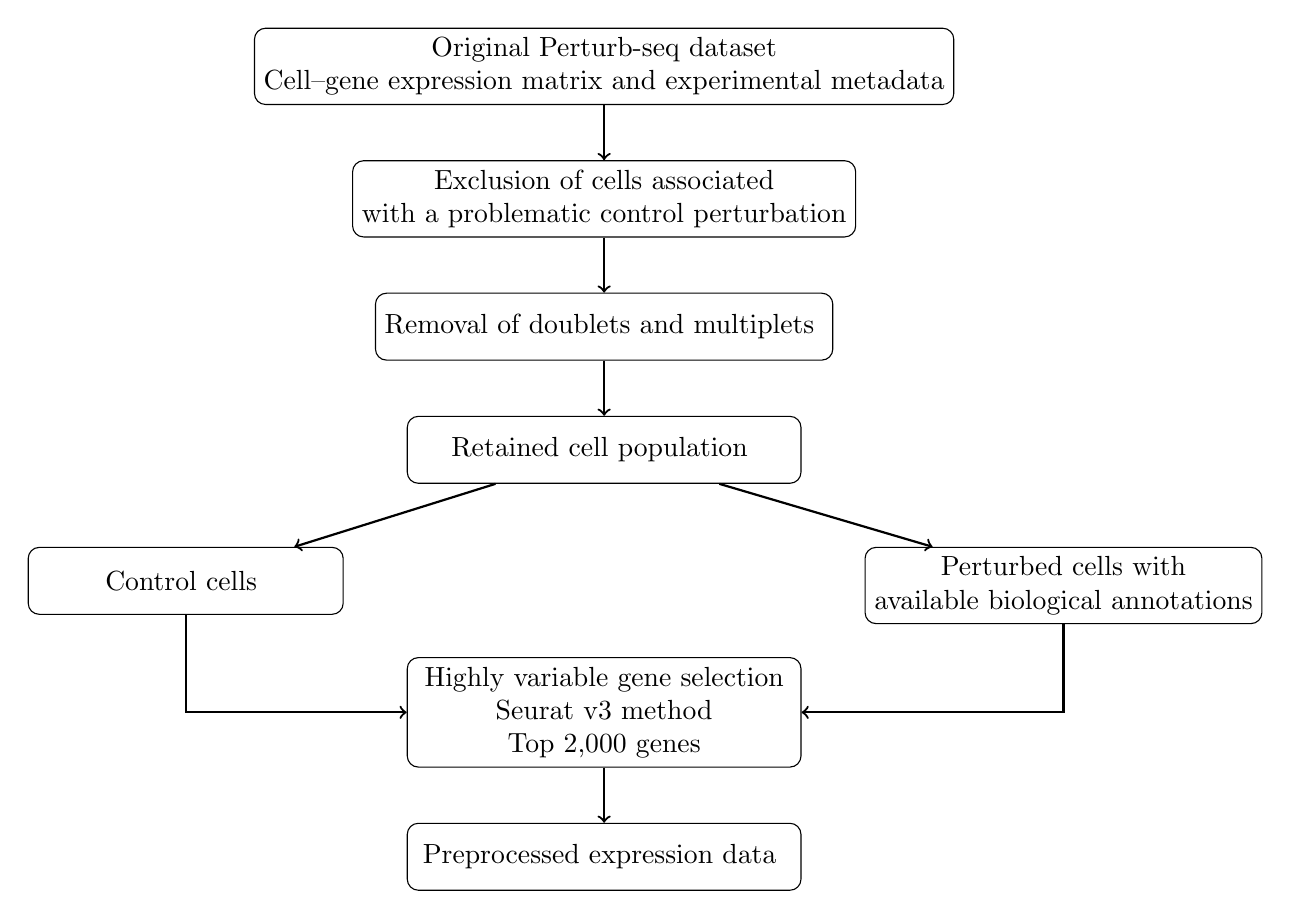
\begin{tikzpicture}[
node distance=7mm,
box/.style={
	rectangle,
	rounded corners,
	draw,
	align=center,
	minimum width=5.0cm,
	minimum height=0.85cm
},
branch/.style={
	rectangle,
	rounded corners,
	draw,
	align=center,
	minimum width=4.0cm,
	minimum height=0.85cm
},
arrow/.style={->, thick}
]

\node[box] (input) {
	Original Perturb-seq dataset\\
	Cell--gene expression matrix and experimental metadata
};

\node[box, below=of input] (specific) {
	Exclusion of cells associated\\
	with a problematic control perturbation
};

\node[box, below=of specific] (doublets) {
	Removal of doublets and multiplets
};

\node[box, below=of doublets] (selection) {
	Retained cell population
};

\node[branch, below left=8mm and 8mm of selection] (controls) {
	Control cells
};

\node[branch, below right=8mm and 8mm of selection] (perturbed) {
	Perturbed cells with\\
	available biological annotations
};

\node[box, below=22mm of selection] (hvg) {
	Highly variable gene selection\\
	Seurat v3 method\\
	Top 2,000 genes
};

\node[box, below=of hvg] (contrastive) {
	Preprocessed expression data
};

\draw[arrow] (input) -- (specific);
\draw[arrow] (specific) -- (doublets);
\draw[arrow] (doublets) -- (selection);

\draw[arrow] (selection) -- (controls);
\draw[arrow] (selection) -- (perturbed);

\draw[arrow] (controls) |- (hvg);
\draw[arrow] (perturbed) |- (hvg);

\draw[arrow] (hvg) -- (contrastive);

\end{tikzpicture} \\

The processed dataset is particularly convenient for downstream single-cell
analysis because the perturbation identity is represented in the cell
metadata. This allows cells to be grouped according to their perturbation
condition and compared with control cells. For example, cells carrying a
non-targeting control can be used to characterize the baseline distribution of
transcriptional states, whereas cells carrying a particular CRISPRa
perturbation can be treated as samples from the corresponding perturbed
distribution.

An important consideration is that the presence of an sgRNA does not
necessarily imply that every cell has undergone an equally strong functional
perturbation. Variable guide efficiency can generate cells that contain a
perturbation label but exhibit little or none of the expected transcriptional
response. This issue is particularly relevant when interpreting cell-level
heterogeneity. Indeed, Weinberger et al.\ developed ContrastiveVI+ partly
because pooled CRISPR screens contain noisy perturbation labels and because
some guide-positive cells can escape the functional consequences of the
perturbation \cite{weinberger2024}. Consequently, perturbation identity should
be interpreted as an experimental assignment rather than as a perfect
measurement of perturbation strength.

%\section{D-SPIN as a framework for perturbation-response modeling}
%
%The high dimensionality of Perturb-seq creates a complementary computational
%challenge. Visualization methods such as PCA and UMAP can reveal similarities
%between perturbations, but they do not directly provide an interpretable
%mechanistic model of the interactions responsible for the observed cellular
%states. D-SPIN (Dimension-scalable Single-cell Perturbation Integration
%Network) was developed to address this problem by constructing probabilistic
%regulatory-network models directly from single-cell perturbation data
%\cite{jiang2023dspin}.
%
%D-SPIN models gene expression, or alternatively groups of co-expressed genes
%called gene programs, using a condition-dependent probabilistic graphical
%model. The central object is a unified interaction network whose nodes
%represent genes or gene programs. Perturbations are represented as
%condition-specific inputs that modify the activity of these nodes. In this
%way, information from many perturbation conditions is integrated into a
%single network rather than treating each perturbation independently
%\cite{jiang2023dspin}.
%
%Conceptually, the model can be written as a probability distribution over
%cellular states,
%
%\begin{equation}
%P(\mathbf{s}\mid\mathbf{h}) =
%\frac{1}{Z(\mathbf{h})}
%\exp\left[
%\frac{1}{2}\mathbf{s}^{T}J\mathbf{s}
%+
%\mathbf{h}^{T}\mathbf{s}
%\right],
%\end{equation}
%
%where $\mathbf{s}$ represents the activity state of the genes or gene
%programs, $J$ represents their pairwise interactions, and $\mathbf{h}$
%represents the perturbation-dependent fields. The normalization factor
%$Z(\mathbf{h})$ ensures that the expression defines a probability
%distribution. This formulation is related to spin-network and Markov-random
%field models. Importantly, $J$ is shared across perturbation conditions,
%whereas $\mathbf{h}$ changes according to the applied perturbation
%\cite{jiang2023dspin}.
%
%This distinction is central to the usefulness of D-SPIN for Perturb-seq.
%Instead of asking only whether perturbation $A$ changes gene $B$, D-SPIN asks
%how perturbations collectively expose the conditional dependencies between
%different components of the cellular regulatory system. Perturbations can
%therefore reveal interactions that are weak or invisible under the
%unperturbed condition. The resulting network provides a representation of the
%cellular system that is both descriptive and generative: it can reproduce
%observed distributions of cell states and can be used to simulate responses
%to perturbations \cite{jiang2023dspin}.

\subsection{Application of D-SPIN to the Norman dataset}

The preprocessed Norman et al.\ dataset is particularly suitable for D-SPIN
because it contains many distinct perturbation conditions measured at
single-cell resolution. A D-SPIN analysis can therefore use the perturbation
identity in the cell metadata as the condition variable while using the
expression matrix as the molecular phenotype.

A practical analysis plan consists of several conceptual stages. 

First, cells and genes should be quality-controlled and the expression matrix transformed into
a representation appropriate for D-SPIN. The D-SPIN implementation expects
log-normalized single-cell expression data and condition labels identifying
the perturbation associated with each cell. Matched control cells are
preferable because they allow perturbation responses to be estimated relative
to the appropriate baseline \cite{jiang2025guide}.

Second, the expression space can either be represented directly at the
gene level or reduced to gene programs. D-SPIN provides an unsupervised
orthogonal non-negative matrix factorization (oNMF) procedure for identifying
such programs, although predefined biologically motivated gene sets can also
be used \cite{jiang2023dspin}.
% \textcolor{red}{Program-level modeling is particularly
%attractive for a master-thesis analysis because it reduces dimensionality and
%often makes the resulting network easier to interpret biologically.}

Third, D-SPIN jointly infers the interaction network and the
perturbation-response vectors. The resulting network can then be
used to determine which genes or programs interact, which perturbations act
on particular parts of the network, and how different perturbations produce
distinct cellular states. In the context of Norman et al., this provides a
complementary perspective to the original genetic-interaction manifold:
whereas Norman et al.\ primarily used transcriptomic similarity to organize
perturbations, D-SPIN attempts to explain those observed responses through a
shared network model.

This distinction also defines an important methodological advantage. Two
perturbations can generate similar transcriptional profiles without acting on
the same regulatory components, while two perturbations with apparently
different profiles may affect different nodes of a common network. D-SPIN's
joint inference of network interactions and perturbation effects is designed
to capture these relationships. The method has specifically been demonstrated
on large Perturb-seq datasets, including K562 perturbation data, where it was
used to investigate regulatory organization and cell-fate responses
\cite{jiang2023dspin}.

Thus, the Norman et al.\ dataset and D-SPIN form a natural methodological
combination. Perturb-seq provides the experimentally controlled,
high-dimensional perturbation-response measurements; the preprocessed
Figshare object provides these measurements in a computationally accessible
form; and D-SPIN provides a probabilistic framework for integrating the
different perturbation conditions into an interpretable network model. The
result is a progression from perturbation to transcriptional
	phenotype and finally to network-level interpretation, which is the
central rationale for using D-SPIN in the present work.

\newpage

\section{Dataset description}

The preprocessed dataset contains single-cell gene expression measurements together with cell-level annotations describing the corresponding perturbation, experimental batch, sequencing quality, and biological response. The expression matrix comprises 27,658 cells and 1,333 retained genes, with expression values represented as floating-point measurements. The matrix is sparse, with a large proportion of zero-valued entries, reflecting the characteristic sparsity of single-cell transcriptomic data.

The perturbation metadata identify 81 distinct guide conditions, including control and targeted perturbations. The experiment contains both single-target and combinatorial perturbations, resulting in a heterogeneous set of perturbation conditions with unequal numbers of cells. This imbalance is relevant for downstream modeling, since perturbations represented by fewer cells provide less information for estimating their associated transcriptional response.

Several quality-control variables are available in the metadata, including read counts, UMI counts, sequencing coverage, and indicators of coverage quality. The retained observations satisfy the available coverage criterion and correspond to individual cells rather than multiplets. These annotations therefore provide information that can be used to assess the reliability of the measurements before applying D-SPIN.

In addition to perturbation identities, the dataset contains biological program annotations assigned to cells. These annotations distinguish control cells from several transcriptional response programs associated with cellular differentiation, growth, apoptosis, and cell-cycle states. They provide an additional biological interpretation of the perturbation responses and can be useful when evaluating the programs or network structures inferred from the expression data.

The retained genes are accompanied by gene identifiers, gene names, and highly-variable-gene annotations. Consequently, the dataset provides a compact representation of the perturbation-induced transcriptional landscape while retaining the metadata required to relate molecular responses to experimental conditions. Together, these characteristics make the dataset suitable for the subsequent D-SPIN analysis, in which perturbation identities define the experimental conditions and gene expression measurements provide the observed molecular responses.

%\section{Blind faith? No, thanks}

\newpage

\section{Running D-SPIN}

A data analysis pipeline designed to apply D-SPIN principles to Weinberger's dataset has been developed using Python. 

The complete code, together with complete instructions set, is available on \href{https://github.com/demetriomagatti/d_spin_oda_thesis/tree/master}{github}. Code is organized in a package-like way, without being a complete python package yet. The codebase is a set of tools and functionalities to wrap and analyze results produced by the protagonist of the work, which is the \texttt{pip} installable DSPIN package \textcolor{red}{reference here to https://github.com/JialongJiang/DSPIN}

\subsection{Analysis summary}

The analysis follows a stepwise workflow aimed at identifying and interpreting transcriptional programs from a perturbation-based single-cell dataset. The overall purpose is to move from the original cellular expression data toward a higher-level description of the biological programs activated or repressed by different perturbations, and to investigate how these programs relate to one another. The analysis combines model validation, identification of characteristic genes, functional interpretation, comparison of program responses, and reconstruction of a network describing relationships between programs. 

Analysis steps summarized hereafter are executed in sequence by the \texttt{main.py} file of the repository. 

\textbf{1. Exploratory data analysis.} The first step consists of loading the previously prepared single-cell dataset and inspecting its general structure. This provides an overview of the available expression data and cell annotations and serves as an initial check that the dataset is suitable for the subsequent analysis. Before constructing the model, the experimental annotations are also standardized. In particular, information describing the perturbation applied to each cell is organized into a consistent sample identifier, control cells are explicitly distinguished from perturbed cells, and information about experimental batches is retained. This preparation ensures that the different perturbations, control observations, and experimental groups can be correctly recognized during the analysis.

\textbf{2. Model generation.} The central part of the workflow is the construction of a model describing transcriptional programs and their relationships. Rather than considering the expression of thousands of genes independently, the analysis seeks to identify groups of genes that tend to vary together and can therefore be interpreted as coherent transcriptional programs. Each program represents a recurring pattern of gene activity that can be associated with particular cellular processes or responses. At the same time, the model captures how strongly these programs respond to the different perturbations in the dataset. The resulting representation therefore provides two complementary perspectives: what each program consists of and how each program behaves across experimental conditions.

\textbf{3. Model validation.} Once the model has been generated, its basic validity is assessed. These checks are intended to ensure that the inferred programs and their associated results are internally consistent and suitable for further interpretation. A specific validation is also performed on the underlying matrix decomposition, verifying that the identified programs and their associated components have been generated appropriately. These steps are important because the subsequent biological conclusions depend on the quality and consistency of the inferred programs.

\textbf{4. Characterization of program-associated genes.} The analysis then focuses on the genes associated with each program. For every program, the genes contributing most strongly to its definition are identified, providing a concise representation of its molecular characteristics. Examining these highly ranked genes offers an initial indication of the biological identity of each program. For example, a group of genes involved in a common cellular process may suggest that the corresponding program represents that process. In addition to these short lists of highly characteristic genes, the analysis retains a complete ranking of genes for every program. This more comprehensive representation is subsequently used to investigate the biological functions associated with each program.

\textbf{5. Relationships between programs.} The relationships between programs are then examined by comparing their overall patterns. Programs that show similar behaviour are expected to have similar response profiles, whereas programs with opposing behaviour may represent contrasting cellular states or biological processes. A correlation analysis is therefore used to identify pairs of programs whose activities are strongly related. The strongest relationships are specifically examined to highlight potentially redundant, closely related, or biologically connected programs. This step helps determine whether the inferred programs represent clearly distinct processes or whether some of them capture related aspects of the same underlying cellular response.

\textbf{6. Functional interpretation of programs.} The biological interpretation of the programs is further developed through enrichment analysis. The complete ranked gene lists are compared with known groups of genes associated with biological functions and processes. The purpose is to determine whether the genes defining a particular program are disproportionately associated with specific biological activities. The results are subsequently summarized to provide an overview of the main functional characteristics of the programs. This allows the analysis to move beyond individual marker genes and assess the broader biological meaning of each transcriptional program.

\textbf{7. Program responses to perturbations.} A substantial part of the analysis is dedicated to understanding how the programs respond to the different perturbations. The relative activity of every program is examined across all experimental conditions, allowing perturbations that strongly activate or suppress particular programs to be identified. The strongest positive and negative responses are extracted to provide a concise overview of the most pronounced effects. This can reveal, for instance, which perturbations are associated with the strongest activation of a particular cellular process and which produce the opposite response.

\textbf{8. Reciprocal and selective responses.} The response patterns are also examined for reciprocal behaviour. This analysis investigates whether some programs tend to increase when others decrease, which may indicate opposing or complementary biological responses. In parallel, summaries of program activation are generated to characterize the overall behaviour of the programs across the perturbation landscape. The selectivity of program activation is also assessed, with the aim of determining whether a program responds broadly to many perturbations or is associated more specifically with a smaller subset of conditions. Together, these analyses provide a more detailed picture of the functional specificity of the inferred programs.

\textbf{9. Clustering of program responses.} The response patterns are subsequently visualized and compared through their correlations. Programs with similar responses across perturbations are grouped together, while programs with substantially different response patterns are separated. A hierarchical clustering analysis is used to organize the programs according to these similarities, providing an intuitive overview of groups of programs that behave in a comparable manner. Importantly, this classification is based on how the programs respond to perturbations rather than solely on the genes that constitute them. Consequently, programs that may have different molecular compositions can nevertheless be recognized as functionally related if they respond similarly to the same experimental perturbations.

\textbf{10. Directed program network.} Finally, the analysis considers the programs as components of a directed network. In this representation, each program is treated as a node, while connections between nodes describe relationships inferred from the model. Weak relationships are filtered out so that the resulting network focuses on the stronger and more meaningful connections. The direction of the relationships is retained, allowing the network to represent not only whether two programs are connected but also the inferred directionality of their association.

\textbf{11. Identification of program modules.} The network is further divided into modules, corresponding to groups of programs that are more strongly interconnected with one another. These modules provide a higher-level view of the organization of the inferred transcriptional programs and may represent groups of biological processes that participate in related cellular responses. The final network visualization therefore integrates several aspects of the preceding analysis into a single representation, showing how individual programs are connected and how they are organized into larger groups. 

%\resizebox{\textwidth}{!}{%
%\begin{tikzpicture}[
%node distance=4mm,
%box/.style={
%	rectangle,
%	rounded corners,
%	draw,
%	align=center,
%	text width=7.5cm,
%	minimum height=0.65cm,
%	font=\small
%},
%branch/.style={
%	rectangle,
%	rounded corners,
%	draw,
%	align=center,
%	text width=4.7cm,
%	minimum height=0.65cm,
%	font=\small
%},
%arrow/.style={->, thick}
%]
%
%% Input
%\node[box] (input) {
%	\textbf{Original Perturb-seq dataset}\\
%	Cell--gene expression matrix and experimental metadata
%};
%
%% Exploratory analysis
%\node[box, below=of input] (eda) {
%	\textbf{Exploratory data analysis}\\
%	Dataset inspection and standardization of perturbation, control, and batch annotations
%};
%
%% Model
%\node[box, below=of eda] (model) {
%	\textbf{Model generation}\\
%	Inference of transcriptional programs and their perturbation responses
%};
%
%% Validation
%\node[box, below=of model] (validation) {
%	\textbf{Model validation}\\
%	Internal consistency checks and validation of matrix decomposition
%};
%
%% Program characterization
%\node[box, below=of validation] (genes) {
%	\textbf{Program-associated genes}\\
%	Identification of characteristic genes and complete gene rankings
%};
%
%% Two branches
%\node[branch, below left=6mm and 7mm of genes] (relationships) {
%	\textbf{Program relationships}\\
%	Correlation analysis and strongest associations
%};
%
%\node[branch, below right=6mm and 7mm of genes] (enrichment) {
%	\textbf{Functional interpretation}\\
%	Gene-set enrichment analysis
%};
%
%% Responses
%\node[box, below=15mm of genes] (responses) {
%	\textbf{Program responses to perturbations}\\
%	Identification of strongest activation and suppression across conditions
%};
%
%% Response branches
%\node[branch, below left=6mm and 7mm of responses] (reciprocal) {
%	\textbf{Reciprocal responses}\\
%	Opposing and complementary program activity
%};
%
%\node[branch, below right=6mm and 7mm of responses] (selectivity) {
%	\textbf{Selective responses}\\
%	Broad versus perturbation-specific activation
%};
%
%% Clustering
%\node[box, below=15mm of responses] (clustering) {
%	\textbf{Clustering of program responses}\\
%	Correlation-based hierarchical clustering
%};
%
%% Network
%\node[box, below=of clustering] (network) {
%	\textbf{Directed program network}\\
%	Strong inferred relationships retained with directionality
%};
%
%% Modules
%\node[box, below=of network] (modules) {
%	\textbf{Program modules}\\
%	Groups of strongly interconnected programs
%};
%
%% Final output
%\node[box, below=of modules] (output) {
%	\textbf{Integrated transcriptional program landscape}\\
%	Programs, functions, perturbation responses, relationships, and modules
%};
%
%% Main workflow
%\draw[arrow] (input) -- (eda);
%\draw[arrow] (eda) -- (model);
%\draw[arrow] (model) -- (validation);
%\draw[arrow] (validation) -- (genes);
%
%% First branch
%\draw[arrow] (genes) -- (relationships);
%\draw[arrow] (genes) -- (enrichment);
%
%\draw[arrow] (relationships) |- (responses);
%\draw[arrow] (enrichment) |- (responses);
%
%% Second branch
%\draw[arrow] (responses) -- (reciprocal);
%\draw[arrow] (responses) -- (selectivity);
%
%\draw[arrow] (reciprocal) |- (clustering);
%\draw[arrow] (selectivity) |- (clustering);
%
%% Final workflow
%\draw[arrow] (clustering) -- (network);
%\draw[arrow] (network) -- (modules);
%\draw[arrow] (modules) -- (output);
%
%\end{tikzpicture}
%}

\subsection{Model specifics}

The DSPIN package allows both to construct single-genes networks and gene programs networks. In the case of a gene program network fit, the package performs an initial oNMF operation to create gene programs and then proceeds to build the directional network. oNMF is per-se an algorithm depending on pseudo-random number generation, thus being subject to output differences if run multiple times. Consequently, the division of genes into gene programs can natively be repeated to verify the stability of the operation starting from different random seeds. The result is a \textit{consensus oNMF}. 

The number of repetitions that generate the consensus result and the number of gene programs to split the genes into can be set by the user. At the time of writing of this thesis, no automatic detection of the optimal number gene programs is available in the DSPIN package, and developers suggest iteravitely increasing the number of gene programs and interpreting results. While acknowledging that the suggested approach is the one that should ultimately be followed for publishable work, both the generation of the consensus and the fitting of the directional network are computationally demanding processes. Given that this thesis represents a first exploration of DSPIN aimed at understanding its theoretical foundations and practical applications, relatively small numbers were used:

\begin{itemize}
	\item iterations for oNMF conseunsus: 25;
	\item gene programs: 20.
\end{itemize}

\subsection{Consensus oNMF results}

For each transcriptional program, the genes were ranked according to their weights in the corresponding oNMF component, with higher weights indicating a stronger association between a gene and the respective program. The three genes with the highest weights were selected to provide a concise representation of the main genes contributing to each inferred program. The resulting top-ranked genes are reported in Table \ref{tab:program_top3_genes}, with the corresponding oNMF weights shown in parentheses. These weights are relative measures of the contribution of each gene to the respective program and were therefore used to identify the genes most strongly associated with each transcriptional component.

\begin{table}[htbp]
	\centering	
%	\fontsize{0.6\dimexpr\the\fontdimen6\font\relax}{1.1\baselineskip}\selectfont
	\smaller[1]
	\renewcommand{\arraystretch}{1.2}
	\resizebox{\textwidth}{!}{%
%		\begin{tabular}{cccc}
		\begin{tabular*}{\linewidth}{@{\extracolsep{\fill}} cccc }
			\hline
			\textbf{Program} & \textbf{Gene} 1 & \textbf{Gene} 2 & \textbf{Gene} 3 \\
			\hline
			1  & YBX1 (0.3064) & ATP5I (0.2258) & PTMA (0.1822) \\
			2  & HIST1H4C (0.3324) & KIAA0101 (0.2744) & TYMS (0.2180) \\
			3  & CKS2 (0.2264) & CENPF (0.2100) & BIRC5 (0.2078) \\
			4  & AP1S2 (0.2596) & EVA1B (0.2554) & ARHGDIB (0.2393) \\
			5  & LST1 (0.2364) & TYROBP (0.2166) & CSF3R (0.2138) \\
			6  & ENO1 (0.2095) & SSBP1 (0.1451) & UFD1L (0.1446) \\
			7  & GYPA (0.3021) & GYPB (0.3013) & HBG2 (0.3006) \\
			8  & UBE2L3 (0.2302) & NDUFS5 (0.2071) & ATP5G3 (0.2006) \\
			9  & HBA1 (0.5772) & HBA2 (0.4449) & HEMGN (0.3868) \\
			10 & SOCS2 (0.3576) & S100A13 (0.3002) & MAP1A (0.2026) \\
			11 & GAL (0.3011) & HBQ1 (0.2639) & HK1 (0.2506) \\
			12 & RPL14 (0.3822) & RPS5 (0.3763) & MT-ND2 (0.3574) \\
			13 & CYCS (0.1853) & SLIRP (0.1836) & PA2G4 (0.1799) \\
			14 & CDK1 (0.3287) & PIF1 (0.3004) & GTSE1 (0.2647) \\
			15 & PLK1 (0.3106) & CDC20 (0.3076) & CCNB1 (0.2950) \\
			16 & ALAS2 (0.3343) & TSC22D1 (0.2918) & AC006262.5 (0.2830) \\
			17 & CLC (0.4520) & SRGN (0.4480) & NCF1 (0.4320) \\
			18 & CD84 (0.5835) & COL9A2 (0.5339) & FYB (0.3678) \\
			19 & WDR43 (0.2623) & NOP16 (0.2397) & GAR1 (0.2277) \\
			20 & RP11-301G19.1 (0.2770) & S100A11 (0.1970) & SH3BGRL3 (0.1945) \\
			\hline
		\end{tabular*}%
	}
		\caption{Top three genes associated with each inferred transcriptional program. Gene strengths correspond to the gene weights assigned by the oNMF model.}
		\label{tab:program_top3_genes}			
\end{table}


\subsubsection{Enrichment}

Following the characterization of the genes associated with each transcriptional program, over-representation analysis (ORA) was performed to investigate the biological processes represented within the inferred programs. For each program, the 100 highest-ranked genes were tested against the Gene Ontology (GO) Biological Process 2023 gene sets using the genes detected in the dataset as the background. GO terms with an adjusted $p$-value below 0.05 were considered significantly enriched. This analysis therefore provided an independent functional characterization of the transcriptional programs based on the biological processes over-represented among their constituent genes.

Several programs displayed highly coherent functional enrichments. ORA results are summarized in Table \ref{tab:ora_summary}.

\textbf{Program 1} was significantly associated with RNA-related processes, including mRNA processing, mRNA splicing via the spliceosome, RNA splicing, and protein--RNA complex assembly. The strongest enrichment was observed for mRNA processing (adjusted $p = 3.09\times10^{-5}$; odds ratio = 11.87), consistent with the presence of RNA-associated genes such as \textit{YBX1}, \textit{SNRPG}, and \textit{SNRPE}. 

\textbf{Program 2} showed a strong DNA replication and repair signature, with significant enrichment for DNA damage response, DNA metabolic process, DNA repair, DNA-templated DNA replication, and double-strand break repair via homologous recombination. DNA-templated DNA replication showed an odds ratio of 35.65, while DNA repair had an adjusted $p$-value of $3.24\times10^{-7}$, supporting the interpretation of this program as a DNA replication and repair-associated state.

\textbf{Program 3} exhibited a strong cell-cycle and mitotic signature. Significant terms included mitotic sister chromatid segregation, regulation of the cell cycle, positive regulation of cell-cycle processes, and mitotic spindle organization. The enrichment for positive regulation of the cell cycle was particularly strong (odds ratio = 23.30; adjusted $p = 3.28\times10^{-10}$). This functional profile was consistent with the presence of genes including \textit{CENPF}, \textit{BIRC5}, \textit{TOP2A}, \textit{TPX2}, and \textit{CCNA2}. 

\textbf{Program 5} showed enrichment for hematopoietic and immune-associated processes, including regulation of T-cell-mediated cytotoxicity and hemopoiesis. These findings were consistent with its expression of genes such as \textit{LST1}, \textit{TYROBP}, \textit{CSF3R}, \textit{MS4A3}, and \textit{CEBPE}.

\textbf{Program 7} displayed a characteristic erythroid and gas-transport signature. Significant terms included oxygen transport, carbon dioxide transport, gas transport, and one-carbon compound transport, all with an adjusted $p$-value of approximately 0.039 and an odds ratio of 25.65. These enrichments were supported by the presence of erythroid-associated genes such as \textit{GYPA}, \textit{GYPB}, \textit{HBG2}, \textit{HBZ}, \textit{HBG1}, and \textit{SLC25A37}. 

\textbf{Program 8} was associated with proteostasis and metabolic processes, including proteasome-mediated ubiquitin-dependent protein catabolism, ubiquitin-dependent protein catabolic processes, proteasomal protein catabolism, and cellular respiration. These enrichments were consistent with genes such as \textit{UBE2L3}, \textit{POMP}, \textit{PSMA7}, \textit{NDUFS5}, and \textit{COX5A}.

\textbf{Program 9} showed enrichment for antigen processing and presentation of endogenous antigens, together with processes related to smooth-muscle and vascular-associated smooth-muscle proliferation. Its gene composition included \textit{HBA1}, \textit{HBA2}, \textit{HEMGN}, \textit{CNN1}, and \textit{AHSP}, indicating a complex blood- and erythroid-associated transcriptional signature. 

\textbf{Program 13} was characterized by mitochondrial processes, including protein targeting to mitochondria, insertion of proteins into the mitochondrial membrane, mitochondrial gene expression, mitochondrial organization, and translation. Protein insertion into the mitochondrial membrane showed an odds ratio of 32.39, while the enrichment of mitochondrial gene expression reached an adjusted $p$-value of 0.0119.

\textbf{Programs 14 and 15} were predominantly associated with cell-cycle and mitotic functions. Although Program 14 also produced an enrichment for antigen processing and presentation, its leading genes, including \textit{CDK1}, \textit{PIF1}, \textit{GTSE1}, \textit{HJURP}, and \textit{KIFC1}, were more consistent with chromosome dynamics and cell-cycle progression. Program 15 showed significant enrichment for regulation of the mitotic metaphase/anaphase transition and positive regulation of microtubule polymerization. The latter process showed a particularly high odds ratio of 51.33 and was supported by genes including \textit{PLK1}, \textit{CDC20}, \textit{CCNB1}, \textit{CENPE}, and \textit{DLGAP5}.

\textbf{Program 17 and Program 18} displayed immune and hematopoietic associated characteristics. Program 17 was associated with antigen processing and presentation and contained genes including \textit{CLC}, \textit{SRGN}, \textit{NCF1}, \textit{CEBPA}, and \textit{PRG2}. Program 18 also showed enrichment for antigen processing and presentation, consistent with genes such as \textit{CD84}, \textit{FYB}, \textit{ITGAM}, and \textit{CD48}. 

\textbf{Program 19} showed a particularly coherent ribosome-related signature, with significant enrichment for ribosome biogenesis, ribonucleoprotein complex biogenesis, and ribosomal large-subunit biogenesis. These findings were consistent with the presence of \textit{WDR43}, \textit{NOP16}, \textit{GAR1}, \textit{RRP1B}, and \textit{DKC1}.

Finally, \textbf{Program 20} was significantly associated with inflammatory and host-defense processes, including positive regulation of the inflammatory response, regulation of the inflammatory response, defense response to bacterium, and positive regulation of defense response. The strongest terms had adjusted $p$-values of approximately $3.06\times10^{-3}$ and odds ratios of 18.49. The presence of genes such as \textit{LAPTM5}, \textit{VIM}, \textit{PYCARD}, and \textit{BTG1} further supported an immune- and stress-associated interpretation.

Not all programs produced significant GO Biological Process enrichments. In particular, programs 4, 6, 10, 11, 12, and 16 did not contain terms that passed the adjusted $p$-value threshold of 0.05. The absence of significant enrichment does not imply that these programs lack biological relevance; rather, their constituent genes did not form sufficiently large or specific overlaps with the tested GO categories under the applied statistical threshold. Their interpretation was therefore based primarily on their gene composition and was considered separately from the ORA results.

Overall, the enrichment analysis demonstrated that a substantial proportion of the inferred transcriptional programs corresponded to coherent biological processes. Programs associated with RNA processing, DNA replication and repair, cell-cycle progression, erythroid function, mitochondrial activity, ribosome biogenesis, and inflammatory responses were identified. These findings provided functional support for the inferred programs and demonstrated that the transcriptional decomposition captured biologically interpretable cellular processes rather than only mathematical patterns in the expression data.

\begin{table}[htbp]
	\centering
	\renewcommand{\arraystretch}{1.25}
	\setlength{\tabcolsep}{6pt}
\begin{tabular*}{\linewidth}{@{\extracolsep{\fill}} cccl }
		\hline
		& \textbf{Program} & \textbf{Main biological processes} & \\
		\hline
		& \enrichedbox\makebox[0.3cm][r]{1}  & RNA processing and RNA splicing & \\
		& \enrichedbox\makebox[0.3cm][r]{2}  & DNA replication, DNA repair and DNA damage response & \\
		& \enrichedbox\makebox[0.3cm][r]{3}  & Cell cycle and mitotic chromosome segregation & \\
		& \notenrichedbox\makebox[0.3cm][r]{4}  & No significant GO Biological Process terms & \\
		& \enrichedbox\makebox[0.3cm][r]{5}  & Hemopoiesis and immune/cytotoxicity-related processes & \\
		& \notenrichedbox\makebox[0.3cm][r]{6}  & No significant GO Biological Process terms & \\
		& \enrichedbox\makebox[0.3cm][r]{7}  & Oxygen, carbon dioxide and gas transport & \\
		& \enrichedbox\makebox[0.3cm][r]{8}  & Proteasomal degradation and cellular respiration & \\
		& \enrichedbox\makebox[0.3cm][r]{9}  & Antigen processing and vascular/smooth muscle-related processes & \\
		& \notenrichedbox\makebox[0.3cm][r]{10} & No significant GO Biological Process terms & \\
		& \notenrichedbox\makebox[0.3cm][r]{11} & No significant GO Biological Process terms & \\
		& \notenrichedbox\makebox[0.3cm][r]{12} & No significant GO Biological Process terms & \\
		& \enrichedbox\makebox[0.3cm][r]{13} & Mitochondrial function and mitochondrial gene expression & \\
		& \enrichedbox\makebox[0.3cm][r]{14} & Antigen processing and presentation & \\
		& \enrichedbox\makebox[0.3cm][r]{15} & Mitotic progression and microtubule organization & \\
		& \notenrichedbox\makebox[0.3cm][r]{16} & No significant GO Biological Process terms & \\
		& \enrichedbox\makebox[0.3cm][r]{17} & Antigen processing and presentation & \\
		& \enrichedbox\makebox[0.3cm][r]{18} & Antigen processing and presentation & \\
		& \enrichedbox\makebox[0.3cm][r]{19} & Ribosome and ribonucleoprotein biogenesis & \\
		& \enrichedbox\makebox[0.3cm][r]{20} & Inflammatory and host-defense responses & \\
		\hline
	\end{tabular*}
	\caption{Summary of GO Biological Process enrichment across the inferred transcriptional programs. A program was considered enriched when at least one GO term had an adjusted $p-\text{value}<0.05$. Overall, 14 of 20 programs showed at least one significantly enriched GO Biological Process term.}
		\label{tab:ora_summary}
	\end{table}


\subsubsection{Programs correlation (cell-level)}

%To further characterize the relationships between the inferred transcriptional programs, Pearson correlations were calculated between their program activity profiles. The resulting correlation matrix is shown in Figure \ref{fig:correlation}. Positive correlations indicate that the activities of two programs tend to increase or decrease together across the analyzed samples, whereas negative correlations indicate opposing patterns of activity.

To further characterize the relationships between the inferred transcriptional programs, Pearson correlations were calculated between their \textbf{cell-level program activity profiles}. In this analysis, each program is represented by its activity across the individual cells in the dataset. Thus, the correlation between two programs measures whether they tend to show similar or opposing activity states in the \textbf{same cells}. Positive correlations indicate that two programs tend to be active in the same cells, whereas negative correlations indicate that high activity of one program tends to be associated with lower activity of the other. Although the cells are assigned to different perturbation conditions, the perturbation label is not the unit of observation in this analysis; the correlations are calculated directly across individual cells. The resulting correlation matrix is shown in Figure \ref{fig:correlation}.

\begin{figure}[h]
	\centering
	\setlength{\abovecaptionskip}{2pt}
	\[
	\begin{array}{c}
	\textbf{Cell-level program correlation}\\[6pt]
	\underset{\text{}}{
		\begin{array}{|c|cccc|}
		\hline
		& P_1 & P_2 & \cdots & P_K\\
		\hline
		c_1 & +1 & 0  & \cdots & +1\\
		c_2 & +1 & +1 & \cdots & 0\\
		c_3 & 0  & +1 & \cdots & +1\\
		c_4 & -1 & 0  & \cdots & -1\\
		\vdots & \vdots & \vdots & & \vdots\\
		c_N & +1 & +1 & \cdots & 0\\
		\hline
		\end{array}}
	\\[8pt]
	\text{Each program is represented by its activity across cells}\\[4pt]
	P_i=(P_{i,c_1},P_{i,c_2},\ldots,P_{i,c_N})\\[8pt]
	\Downarrow\\[-2pt]
	r_{ij}=\operatorname{cor}(P_i,P_j)\\[8pt]
	\textbf{Interpretation:}\\
	\text{similar or opposing activity of two programs in the same cells}
	\end{array}
	\]
	\caption{Cell-level program correlation. Pearson correlations are calculated between inferred program activity profiles across individual cells. Each program is therefore represented by its activity values across the cells in the dataset. Positive correlations indicate that two programs tend to show similar activity states in the same cells, whereas negative correlations indicate opposing activity patterns.}
	\label{fig:cell_level_program_correlation}
\end{figure} 

Several pairs of programs showed relatively strong positive correlations. The strongest association was observed between \textbf{Programs 1 and 13} ($r = 0.79$). Program 1 was characterized by RNA processing and splicing, whereas Program 13 was associated primarily with mitochondrial function and mitochondrial gene expression. Other strong positive correlations included \textbf{Programs 6 and 8} ($r = 0.73$), \textbf{Programs 13 and 19} ($r = 0.71$), and \textbf{Programs 5 and 20} ($r = 0.68$). Programs 13 and 19 were particularly notable because both showed positive associations with several other programs, with Program 19, which was characterized by ribosome and ribonucleoprotein biogenesis, correlating with Program 13 at $r = 0.71$ and with Program 1 at $r = 0.63$.

The cell-cycle-associated programs also displayed substantial positive correlations. Programs 3 and 14 showed a correlation of $r = 0.66$, while Programs 3 and 15 showed a correlation of $r = 0.66$. This pattern is consistent with the functional characterization of these programs, as Program 3 was associated with cell-cycle and mitotic processes, while Programs 14 and 15 were also characterized by genes involved in chromosome dynamics, mitotic progression, and microtubule organization. The correlation between Programs 14 and 15 was comparatively lower but still positive ($r = 0.45$).

Several negative correlations were also observed. The strongest negative associations involved \textbf{Programs 6 and 16} ($r = -0.48$) and \textbf{Programs 13 and 20} ($r = -0.48$). Program 20, which was enriched for inflammatory and host-defense processes, also showed negative correlations with Programs 1 ($r = -0.46$), 11 ($r = -0.46$), and 7 ($r = -0.43$). Similarly, Program 5, which was associated with hematopoietic and immune-related processes, showed negative correlations with Programs 1 ($r = -0.45$), 13 ($r = -0.46$), and 19 ($r = -0.36$).

The correlation structure therefore revealed groups of programs with coordinated activity as well as programs exhibiting opposing activity patterns. In particular, positive correlations were evident among several programs associated with proliferative, biosynthetic, mitochondrial, and ribosomal processes, whereas some immune- and hematopoietic-associated programs displayed negative associations with these transcriptional states. These relationships provide an additional perspective on the organization of the inferred programs, complementing the independent functional characterization obtained through GO enrichment analysis.

Importantly, correlations between program activities describe statistical co-variation and should not be interpreted as evidence of direct regulatory interactions or causal relationships between programs. The observed associations may instead reflect shared cellular states, common variation across samples, or changes in the relative representation of different cellular populations.

\begin{figure}[h]
	\centering
	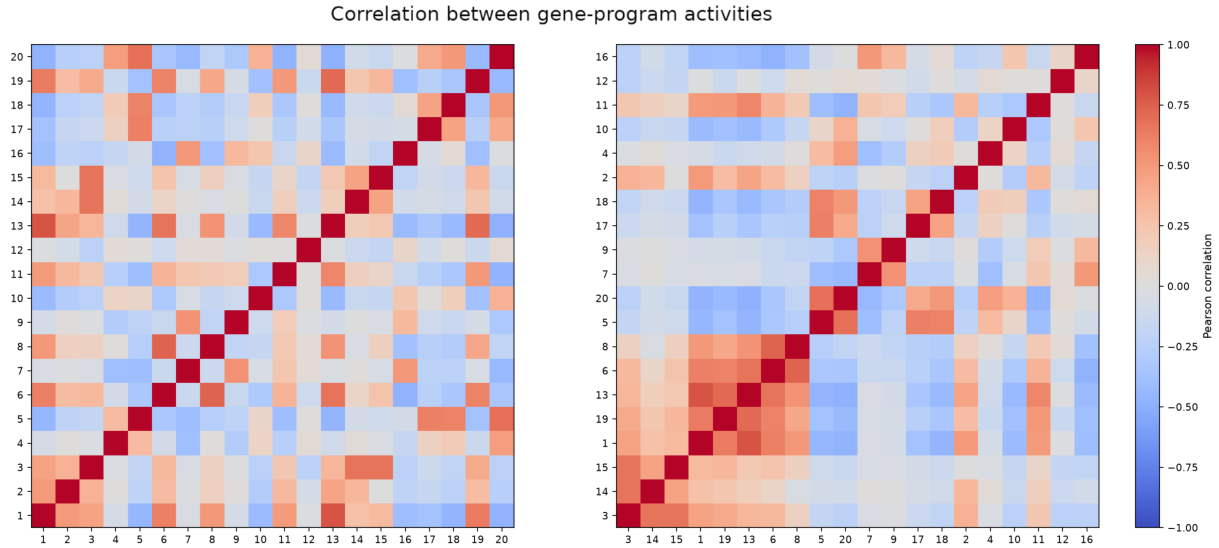
\includegraphics[width=1\textwidth]{img/correlation.pdf}
	\caption{Program correlation. Unordered program list (left), programs grouped according to enrichment analysis (right).}
	\label{fig:correlation}
\end{figure}

\subsection{Relative responses to perturbations}

To characterize the effects of the perturbations on the inferred transcriptional programs, we analyzed the relative-response matrix generated by D-SPIN. In this analysis, the relative response represents the perturbation-associated change in the inferred program response relative to the corresponding control response. Positive values therefore indicate an increased relative response, whereas negative values indicate a decreased relative response. The resulting response matrix is shown in Figure \ref{fig:relative_responses}. \\

\begin{figure}[h]
	\centering
	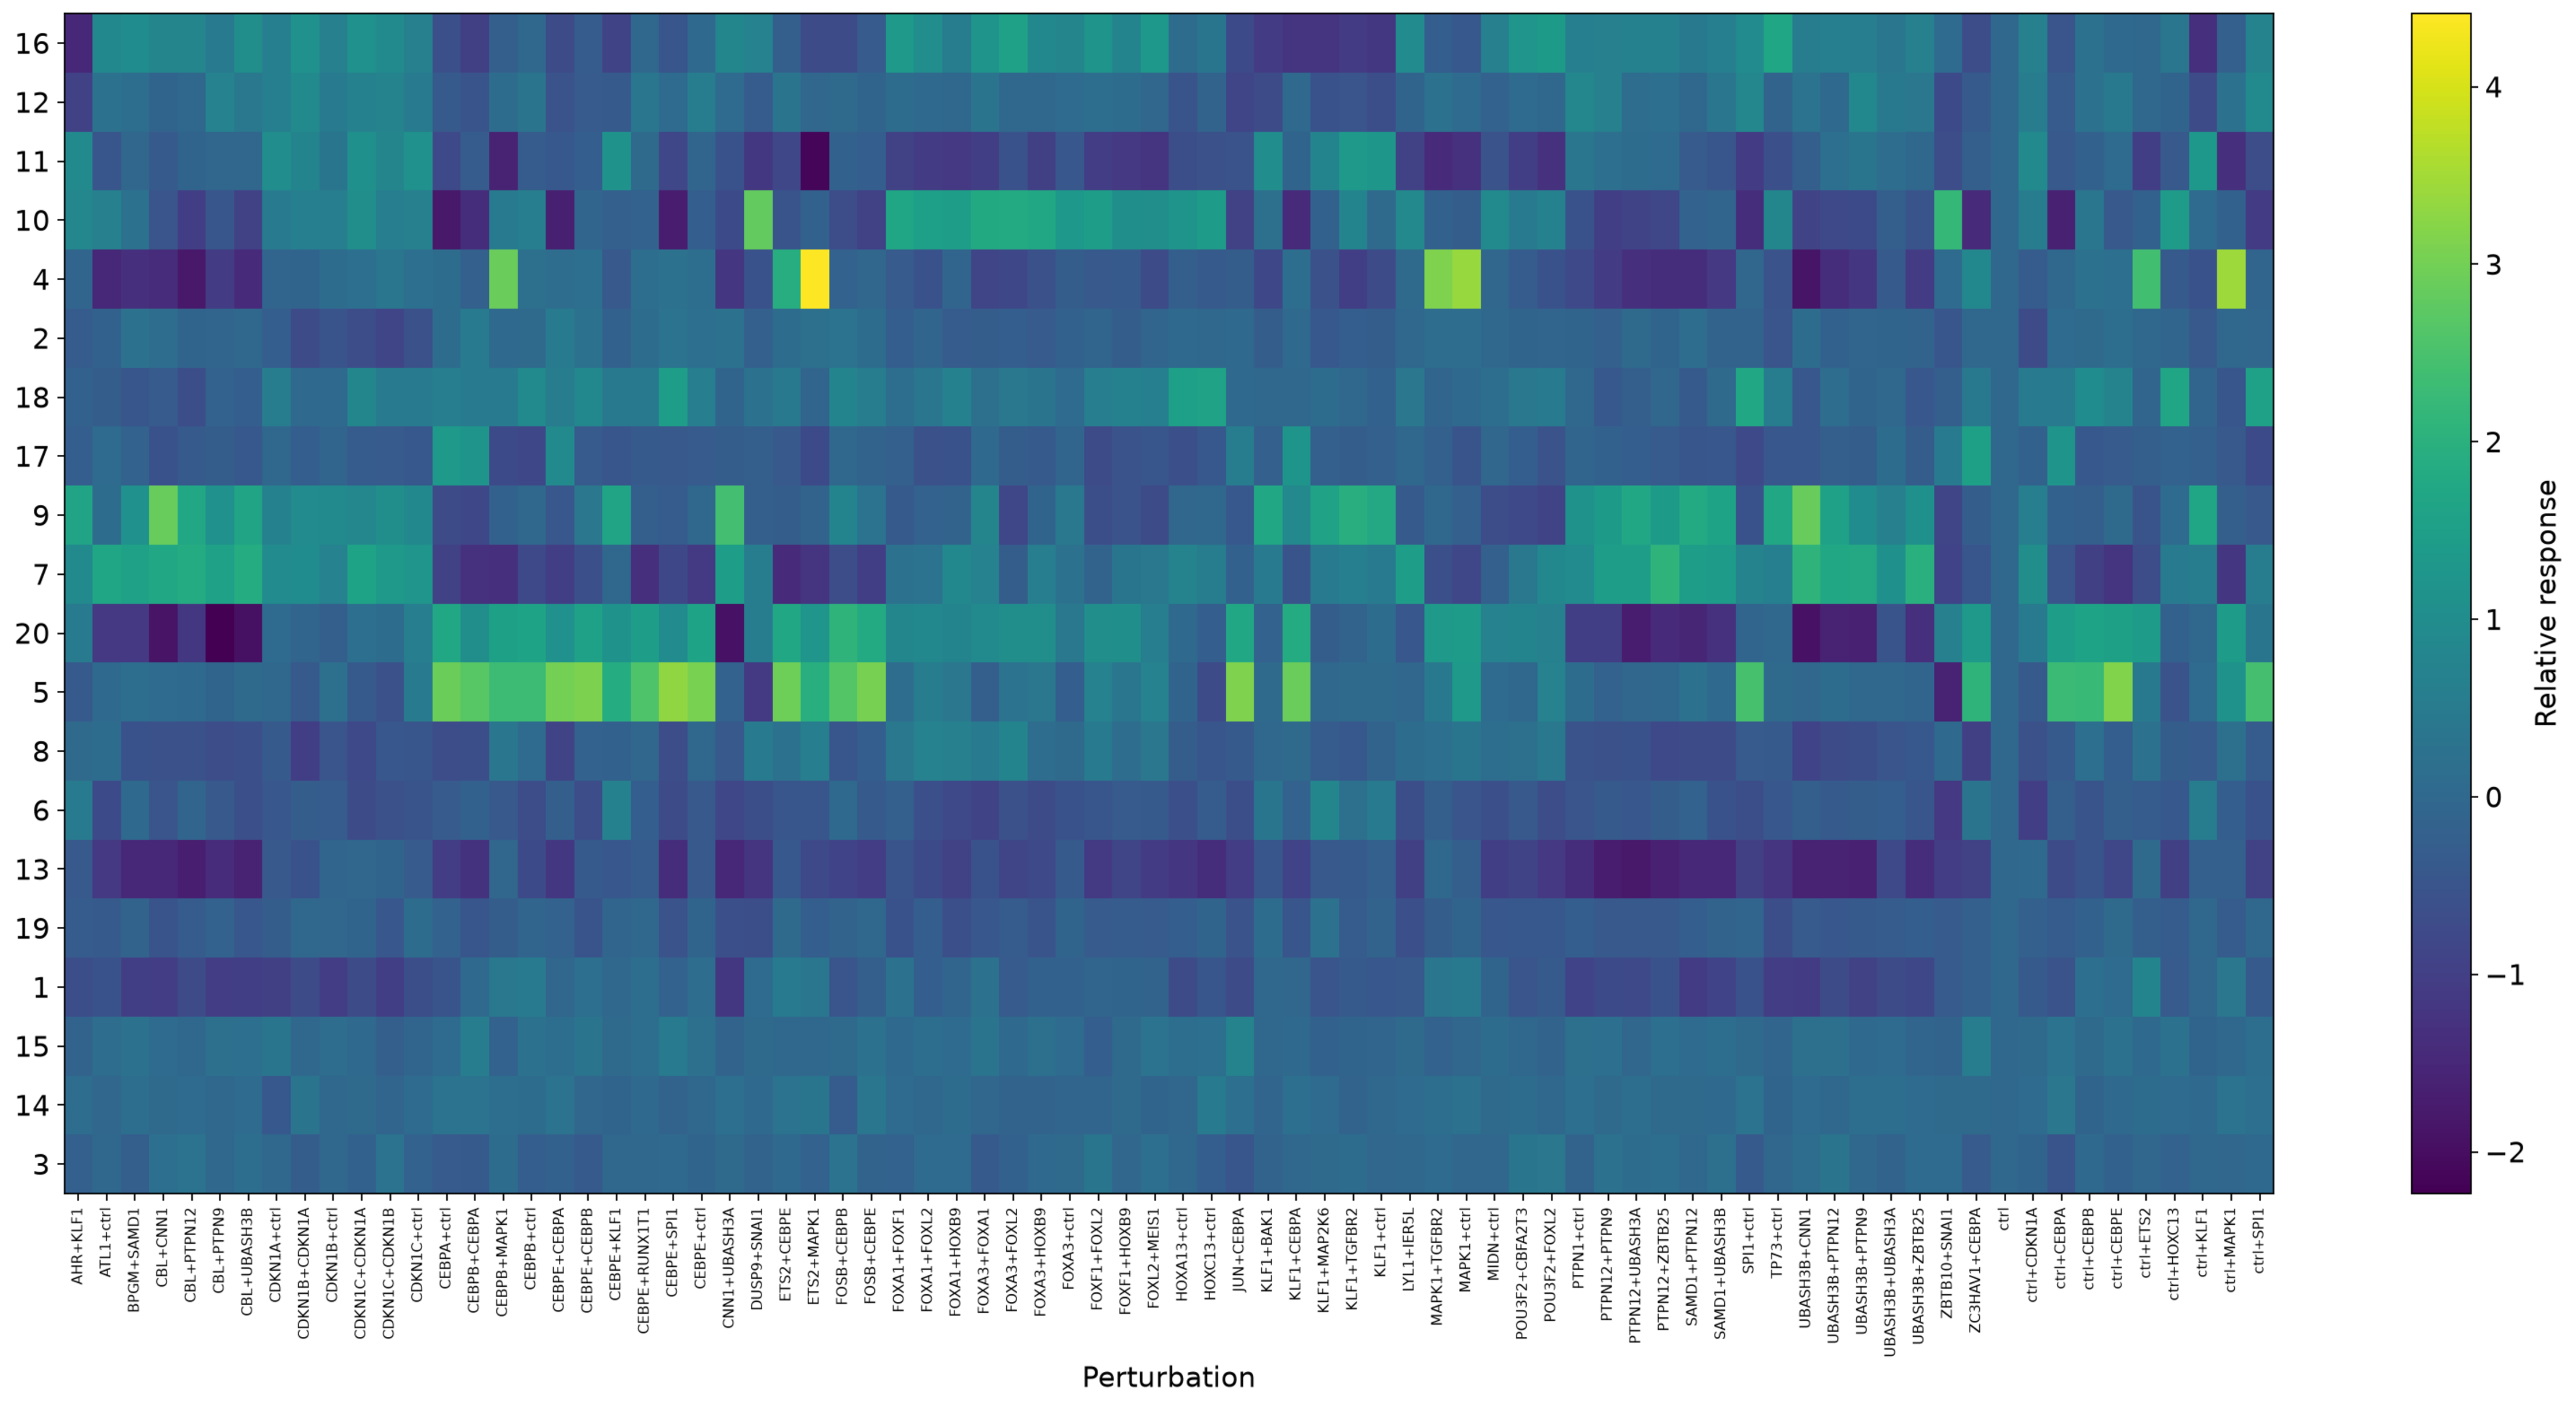
\includegraphics[width=1\textwidth]{img/relative_responses.pdf}
	\caption{Relative responses of the inferred transcriptional programs to perturbations. Rows correspond to transcriptional programs and columns to perturbations.}
	\label{fig:relative_responses}
\end{figure} \\

The distribution of relative responses revealed substantial differences in both the magnitude and selectivity of perturbation effects. Across the analyzed perturbations, \textbf{Program 5} showed the highest mean relative response (0.7873) and was positive for 55 perturbations. Its strongest responses were observed for CEBPE+SPI1 (3.3028), ctrl+CEBPE (3.1515), and JUN+CEBPA (3.1377). Program 5 was also strongly activated by several other CEBP-associated perturbations, including CEBPE+CEBPA (3.0262), CEBPE+CEBPB (3.1081), and CEBPB+CEBPA (2.6856).

\textbf{Program 9} showed the second-highest mean response (0.4826) and was positive for 43 perturbations. Its strongest responses were observed for CBL+CNN1 (2.8713), UBASH3B+CNN1 (2.8543), and CNN1+UBASH3A (2.4281). A related pattern was observed for \textbf{Program 7}, which was positive for 49 perturbations and reached its highest responses for UBASH3B+CNN1 (2.0836), PTPN12+ZBTB25 (2.0787), and UBASH3B+ZBTB25 (1.9772). These profiles indicate recurrent responses involving Programs 7 and 9 across several perturbations affecting CBL-, UBASH3B-, PTPN12-, and CNN1-associated signaling.

In contrast, some programs showed strong responses restricted to a smaller subset of perturbations. \textbf{Program 4} reached the highest individual relative-response value in the dataset for ETS2+MAPK1 (4.4116), followed by ctrl+MAPK1 (3.4472), MAPK1+ctrl (3.3823), and MAPK1+TGFBR2 (3.1298). Despite these large responses, Program 4 was positive for only 24 perturbations and had a negative mean response (-0.1331), indicating that its strong responses were concentrated in a subset of perturbations. Similarly, \textbf{Program 10} showed its strongest response for DUSP9+SNAI1 (2.8047), followed by ZBTB10+SNAI1 (2.2042) and FOXA3+FOXL2 (1.8375).

Other programs displayed recurrent responses across several perturbation classes. Program 18 was positive for 51 perturbations, with its highest responses observed for SPI1+ctrl (1.7518), ctrl+HOXC13 (1.6760), and HOXC13+ctrl (1.5861). Program 16 was positive for 52 perturbations and reached its highest responses for TP73+ctrl (1.7040), FOXA3+FOXL2 (1.5630), and POU3F2+FOXL2 (1.3863). Program 20 was positive for 49 perturbations and was strongest for FOSB+CEBPB (2.0790), KLF1+CEBPA (1.8429), and FOSB+CEBPE (1.8379).

A summary of the strongest perturbation responses for each program is provided in Table \ref{tab:program_relative_response_summary}. In addition to the three strongest responses, the table reports the mean and standard deviation of the response distribution and the number of perturbations with a positive response.

\begin{table}[htbp]
	\centering
	\smaller[3]
	\renewcommand{\arraystretch}{1.2}
	\resizebox{\textwidth}{!}{%
		\begin{tabular*}{\linewidth}{@{\extracolsep{\fill}} cccc cc}
			\hline
			\textbf{Program} & \textbf{Top response 1} & \textbf{Top response 2} & \textbf{Top response 3} &
			\textbf{Mean} & \textbf{SD} \\
			\hline
			1  & ctrl+ETS2 (0.7657) & CEBPB+ctrl (0.5168) & ETS2+CEBPE (0.4836) & -0.3453 & 0.4692 \\
			2  & CEBPE+CEBPA (0.5327) & CEBPB+CEBPA (0.5023) & FOSB+CEBPB (0.3007) & -0.0840 & 0.2603 \\
			3  & POU3F2+FOXL2 (0.3877) & POU3F2+CBFA2T3 (0.3601) & FOXF1+FOXL2 (0.3579) & -0.0218 & 0.1930 \\
			4  & ETS2+MAPK1 (4.4116) & ctrl+MAPK1 (3.4472) & MAPK1+ctrl (3.3823) & -0.1331 & 1.1839 \\
			5  & CEBPE+SPI1 (3.3028) & ctrl+CEBPE (3.1515) & JUN+CEBPA (3.1377) & 0.7873 & 1.2674 \\
			6  & KLF1+MAP2K6 (0.8133) & CEBPE+KLF1 (0.6938) & ctrl+KLF1 (0.5691) & -0.3480 & 0.3649 \\
			7  & UBASH3B+CNN1 (2.0836) & PTPN12+ZBTB25 (2.0787) & UBASH3B+ZBTB25 (1.9772) & 0.3836 & 1.0169 \\
			8  & FOXA3+FOXL2 (0.7547) & FOXA1+FOXL2 (0.7146) & FOXA1+HOXB9 (0.6534) & -0.1903 & 0.4412 \\
			9  & CBL+CNN1 (2.8713) & UBASH3B+CNN1 (2.8543) & CNN1+UBASH3A (2.4281) & 0.4826 & 0.9597 \\
			10 & DUSP9+SNAI1 (2.8047) & ZBTB10+SNAI1 (2.2042) & FOXA3+FOXL2 (1.8375) & 0.1028 & 1.0250 \\
			11 & KLF1+TGFBR2 (1.3622) & ctrl+KLF1 (1.2986) & KLF1+ctrl (1.2732) & -0.2596 & 0.7662 \\
			12 & CDKN1B+CDKN1A (0.9335) & ctrl+SPI1 (0.9255) & UBASH3B+PTPN9 (0.8604) & 0.0818 & 0.4323 \\
			13 & ctrl+ETS2 (0.0718) & ctrl+CDKN1A (0.0434) & ctrl (0.0000) & -0.8484 & 0.5095 \\
			14 & HOXC13+ctrl (0.5149) & ctrl+CEBPA (0.4045) & FOSB+CEBPE (0.3799) & 0.0778 & 0.1551 \\
			15 & JUN+CEBPA (0.7405) & CEBPB+CEBPA (0.5811) & ZC3HAV1+CEBPA (0.5447) & 0.1024 & 0.1787 \\
			16 & TP73+ctrl (1.7040) & FOXA3+FOXL2 (1.5630) & POU3F2+FOXL2 (1.3863) & 0.2708 & 0.7792 \\
			17 & ZC3HAV1+CEBPA (1.5472) & CEBPA+ctrl (1.3583) & CEBPB+CEBPA (1.2143) & -0.1744 & 0.4808 \\
			18 & SPI1+ctrl (1.7518) & ctrl+HOXC13 (1.6760) & HOXC13+ctrl (1.5861) & 0.3061 & 0.5298 \\
			19 & KLF1+MAP2K6 (0.2452) & CDKN1C+ctrl (0.1253) & KLF1+BAK1 (0.1220) & -0.2596 & 0.1986 \\
			20 & FOSB+CEBPB (2.0790) & KLF1+CEBPA (1.8429) & FOSB+CEBPE (1.8379) & 0.2874 & 1.1542 \\
			\hline
		\end{tabular*}%
	}
	\caption{Summary of relative responses for the inferred transcriptional programs. For each program, the three perturbations with the highest relative-response scores are shown together with their scores. Mean response, standard deviation (SD), and the number of perturbations with a positive response are also reported.}
	\label{tab:program_relative_response_summary}
\end{table}

The degree to which individual perturbations preferentially affected a single program was assessed by comparing the highest and second-highest relative-response scores. The ten perturbations with the largest differences are shown in Table \ref{tab:program_response_selectivity}. The largest separation was observed for \textbf{ETS2+MAPK1}, for which Program 4 reached 4.4116 compared with 1.9615 for Program 5, corresponding to a difference of 2.4501. This was followed by DUSP9+SNAI1, for which Program 10 (2.8047) exceeded Program 16 (0.7025) by 2.1022. Similarly, the two MAPK1 control orientations, ctrl+MAPK1 and MAPK1+ctrl, showed strong selectivity for Program 4, with differences of 2.0068 and 1.9762, respectively. CEBPE-associated perturbations also showed substantial selectivity for Program 5, particularly CEBPE+CEBPA (difference = 1.9001) and CEBPE+SPI1 (difference = 1.8399).

\begin{table}[htbp]
	\centering
	\smaller[1]
	\renewcommand{\arraystretch}{1.2}
	\resizebox{\textwidth}{!}{%
		\begin{tabular*}{\linewidth}{@{\extracolsep{\fill}} lccccc}
			\hline
			\textbf{Perturbation} & \textbf{Top program} & \textbf{Top score} &
			\textbf{Second program} & \textbf{Second score} & \textbf{Top--second} \\
			\hline
			ETS2+MAPK1   & Program 4  & 4.4116 & Program 5  & 1.9615 & 2.4501 \\
			DUSP9+SNAI1  & Program 10 & 2.8047 & Program 16 & 0.7025 & 2.1022 \\
			ctrl+MAPK1   & Program 4  & 3.4472 & Program 20 & 1.4404 & 2.0068 \\
			MAPK1+ctrl   & Program 4  & 3.3823 & Program 20 & 1.4061 & 1.9762 \\
			CEBPE+CEBPA  & Program 5  & 3.0262 & Program 20 & 1.1261 & 1.9001 \\
			CEBPE+SPI1   & Program 5  & 3.3028 & Program 18 & 1.4630 & 1.8399 \\
			MAPK1+TGFBR2 & Program 4  & 3.1298 & Program 20 & 1.3638 & 1.7660 \\
			ctrl+CEBPE   & Program 5  & 3.1515 & Program 20 & 1.5536 & 1.5979 \\
			ZBTB10+SNAI1 & Program 10 & 2.2042 & Program 20 & 0.6646 & 1.5395 \\
			CEBPE+CEBPB  & Program 5  & 3.1081 & Program 20 & 1.5792 & 1.5289 \\
			\hline
		\end{tabular*}%
	}
	\caption{Most selective perturbation responses. Perturbations are ranked by the difference between their highest and second-highest program relative-response scores.}
	\label{tab:program_response_selectivity}
\end{table}

As a quality-control measure, reciprocal perturbation representations were compared to assess the symmetry of the inferred responses. Perturbations represented as both \textit{gene+ctrl} and \textit{ctrl+gene} were expected to produce similar program-response profiles if the ordering of the two components did not substantially affect the inferred response. Correlations between reciprocal profiles were high for all eight tested pairs, ranging from $r=0.840$ for CDKN1A to $r=0.987$ for CEBPE. The highest correlations were observed for CEBPE ($r=0.987$), SPI1 ($r=0.985$), MAPK1 ($r=0.984$), KLF1 ($r=0.981$), and CEBPA ($r=0.980$). CDKN1A showed the lowest correlation among the reciprocal pairs ($r=0.840$), while CEBPB and HOXC13 also showed high concordance ($r=0.964$ and $r=0.968$, respectively). The corresponding RMSE values ranged from 0.125 for KLF1 to 0.304 for CDKN1A.

These reciprocal comparisons were used primarily as a quality control check of response symmetry. The high correlations observed across the reciprocal representations indicate that the overall program-response profiles were generally preserved when the order of the perturbation and control labels was reversed. The complete reciprocal comparisons are reported in Table \ref{tab:reciprocal_response_qc}.

\begin{table}[htbp]
	\centering
	\smaller[1]
	\renewcommand{\arraystretch}{1.2}
	\resizebox{\textwidth}{!}{%
		\begin{tabular*}{\linewidth}{@{\extracolsep{\fill}} lllccc}
			\hline
			\textbf{Pair 1} & \textbf{Pair 2} & \textbf{Correlation} &
			\textbf{RMSE} & \textbf{Maximum absolute difference} \\
			\hline
			CEBPE+ctrl  & ctrl+CEBPE  & 0.9869 & 0.1454 & 0.4373 \\			
			SPI1+ctrl   & ctrl+SPI1   & 0.9850 & 0.1966 & 0.4008 \\
			MAPK1+ctrl  & ctrl+MAPK1  & 0.9839 & 0.1777 & 0.4714 \\
			KLF1+ctrl   & ctrl+KLF1   & 0.9809 & 0.1252 & 0.3752 \\			
			CEBPA+ctrl  & ctrl+CEBPA  & 0.9796 & 0.2740 & 0.6092 \\
			HOXC13+ctrl & ctrl+HOXC13 & 0.9677 & 0.1785 & 0.4288 \\
			CEBPB+ctrl  & ctrl+CEBPB  & 0.9642 & 0.2022 & 0.4082 \\
			CDKN1A+ctrl & ctrl+CDKN1A & 0.8398 & 0.3044 & 0.6164 \\			
			\hline
		\end{tabular*}%
	}
	\caption{Reciprocal perturbation QC. Correlation, root mean squared error (RMSE), and maximum absolute difference between the complete program-response profiles of reciprocal perturbation representations.}
	\label{tab:reciprocal_response_qc}
\end{table}

Taken together, the relative-response analysis identified both broadly responsive programs and perturbation-specific response patterns. Program 5 showed the broadest positive response, while Programs 4, 9, and 10 exhibited particularly strong responses to specific groups of perturbations. The selectivity analysis further distinguished perturbations with concentrated responses from those affecting multiple programs more evenly. Finally, the reciprocal analysis provided a QC assessment showing high concordance between alternative representations of the same single perturbation, supporting the consistency of the inferred relative-response profiles.


\subsection{Programs correlation (relative responses)}

%The relative-response profiles and program correlation structure were considered jointly to examine how perturbations were distributed across the inferred transcriptional programs. While the relative-response analysis identifies the programs most strongly affected by individual perturbations, the correlation analysis evaluates whether different programs tend to show coordinated or opposing responses across perturbations. Thus, correlations provide a complementary view of the response structure identified in the perturbation analysis.

The relative-response profiles and their correlation structure were considered jointly to examine how perturbations were distributed across the inferred transcriptional programs. In contrast to the cell-level program correlations described above, this analysis was performed on the \textbf{relative-response profiles of the programs across perturbation conditions}. Here, each program is represented by one relative-response value for each perturbation, obtained from the inferred perturbation responses relative to the corresponding control. Pearson correlation therefore evaluates whether two programs show similar or opposing \textbf{relative-response patterns across perturbations}. Thus, while the cell-level correlation analysis asks whether two programs tend to be active in the same cells, the relative-response correlation asks whether the inferred responses of two programs tend to increase or decrease together across the same perturbation conditions. \\

\begin{figure}[h]
	\centering
	\setlength{\abovecaptionskip}{2pt}
	\[
	\begin{array}{c}
	\textbf{Relative-response correlation}\\[6pt]
	\underset{\text{}}{
		\begin{array}{|c|cccc|}
		\hline
		& \mathrm{Pert}_1 & \mathrm{Pert}_2 & \cdots & \mathrm{Pert}_M\\
		\hline
		P_1 & 2.5 & 0.3 & \cdots & -1.2\\
		P_2 & 2.1 & 0.5 & \cdots & -0.8\\
		\vdots & \vdots & \vdots & & \vdots\\
		P_K & 0.4 & 1.8 & \cdots & 0.2\\
		\hline
		\end{array}}
	\\[8pt]
	\text{Each program is represented by its relative-response profile across perturbations}\\[4pt]
	R_i=(R_{i,1},R_{i,2},\ldots,R_{i,M})\\[8pt]
	\Downarrow\\[-2pt]
	r_{ij}=\operatorname{cor}(R_i,R_j)\\[8pt]
	\textbf{Interpretation:}\\
	\text{similar or opposing relative responses to perturbations}
	\end{array}
	\]
	\caption{Correlation of relative-response profiles. Pearson correlations are calculated between the relative-response profiles of inferred programs across perturbation conditions. Each program is represented by one inferred relative-response value for each perturbation. Positive correlations indicate that two programs tend to show similar response patterns across perturbations, whereas negative correlations indicate opposing response patterns.}
	\label{fig:relative_response_correlation}
\end{figure} \\

Several of the strongest program correlations were consistent with recurrent patterns observed in the relative-response profiles. \textbf{Programs 7 and 9} showed a positive correlation of $r=0.63$ and were both frequently among the strongest responses to perturbations involving CBL, UBASH3B, PTPN12, and CNN1. For example, CBL+CNN1 showed strong responses in Programs 9 and 7 (2.8713 and 1.7399, respectively), while UBASH3B+CNN1 showed responses of 2.8543 and 2.0836. The positive correlation between these programs therefore reflects a recurrent tendency for them to respond together across the perturbation set.

A similar relationship was observed among \textbf{Programs 1, 4, and 20}. Program 1 correlated positively with Program 4 ($r=0.66$) and Program 20 ($r=0.75$), while Programs 4 and 20 were also positively correlated ($r=0.62$). Program 4, however, showed a more selective response pattern, with its strongest responses concentrated in MAPK1- and ETS2-containing perturbations. ETS2+MAPK1 produced the highest Program 4 response in the dataset (4.4116), followed by ctrl+MAPK1 (3.4472), MAPK1+ctrl (3.3823), and MAPK1+TGFBR2 (3.1298). Program 20, in contrast, showed recurrent responses across several perturbations, particularly FOSB- and CEBP-associated combinations, including FOSB+CEBPB (2.0790), KLF1+CEBPA (1.8429), and FOSB+CEBPE (1.8379). The positive correlations between these programs indicate that their responses varied in a coordinated manner across perturbations, despite differences in the perturbations producing their strongest individual responses.

\textbf{Program 5} showed a positive correlation with Program 20 ($r=0.63$) and with Program 2 ($r=0.60$). This relationship was particularly relevant to the CEBP-associated perturbations, for which Program 5 was repeatedly the dominant response. CEBPE+SPI1, ctrl+CEBPE, CEBPE+CEBPA, and CEBPE+CEBPB all showed strong Program 5 responses, while Program 20 was frequently the second-highest response in the same perturbation profiles. The positive correlation between Programs 5 and 20 is therefore consistent with the recurrent co-occurrence of these responses across CEBP-associated perturbations.

The correlation structure also highlighted several pairs of programs with opposing response patterns. The strongest negative correlation in the matrix was observed between \textbf{Programs 7 and 20} ($r=-0.87$). Program 7 was frequently strongly represented among CBL-, UBASH3B-, PTPN12-, and CNN1-associated perturbations, whereas Program 20 was prominent in several CEBP-, FOSB-, and related perturbations. Program 7 also showed strong negative correlations with Program 1 ($r=-0.76$), Program 5 ($r=-0.70$), and Program 4 ($r=-0.68$), indicating that perturbations producing strong responses in Program 7 tended, across the dataset, to show lower relative responses in these programs.

A similarly strong inverse relationship was observed between \textbf{Programs 9 and 20} ($r=-0.68$). This is notable because Program 9 was one of the most broadly responsive programs and was particularly strong in the CBL- and UBASH3B-associated perturbations, whereas Program 20 was more prominent in perturbations such as FOSB+CEBPB and KLF1+CEBPA. Program 9 also showed a negative correlation with Program 18 ($r=-0.50$), while Program 18 was most strongly associated with SPI1+ctrl and HOXC13-containing perturbations. These relationships suggest that distinct perturbation classes can produce contrasting program-response profiles rather than simply differing in the magnitude of a common response.

Other correlations were consistent with more specific response patterns. Programs 8 and 10 were positively correlated ($r=0.58$), and both were represented among the strongest responses of several FOXA-associated perturbations. Program 10 additionally showed particularly strong responses to the two SNAI1-containing perturbations, reaching 2.8047 for DUSP9+SNAI1 and 2.2042 for ZBTB10+SNAI1. Programs 12 and 16 also showed a positive correlation ($r=0.58$), with Program 16 showing strong responses in TP73+ctrl, FOXA3+FOXL2, and POU3F2+FOXL2, while Program 12 reached its highest response for CDKN1B+CDKN1A (0.9335).

The negative correlation between \textbf{Programs 6 and 16} ($r=-0.61$) provides another example of contrasting response behavior. Program 6 was most strongly represented by KLF1+MAP2K6 (0.8133) and related KLF1-associated perturbations, whereas Program 16 reached its highest response for TP73+ctrl (1.7040) and showed substantial responses among several FOXA- and POU3F2-associated perturbations. The opposing response patterns captured by the correlation analysis therefore complement the perturbation-specific profiles identified from the relative-response matrix.

Overall, combining the two analyses revealed a structured organization of perturbation responses. Some programs, such as Programs 7 and 9 and Programs 5 and 20, frequently responded together across perturbations and consequently showed positive correlations. Other programs, particularly Programs 7 and 20, Programs 1 and 7, and Programs 9 and 20, showed strong opposing correlations, reflecting contrasting patterns of response across the perturbation set. The dendrogram summarizes the hierarchical similarity of program-response profiles across perturbations, using correlation-derived distances (Figure \ref{fig:dendogram}).

\begin{figure}[h]
	\centering
	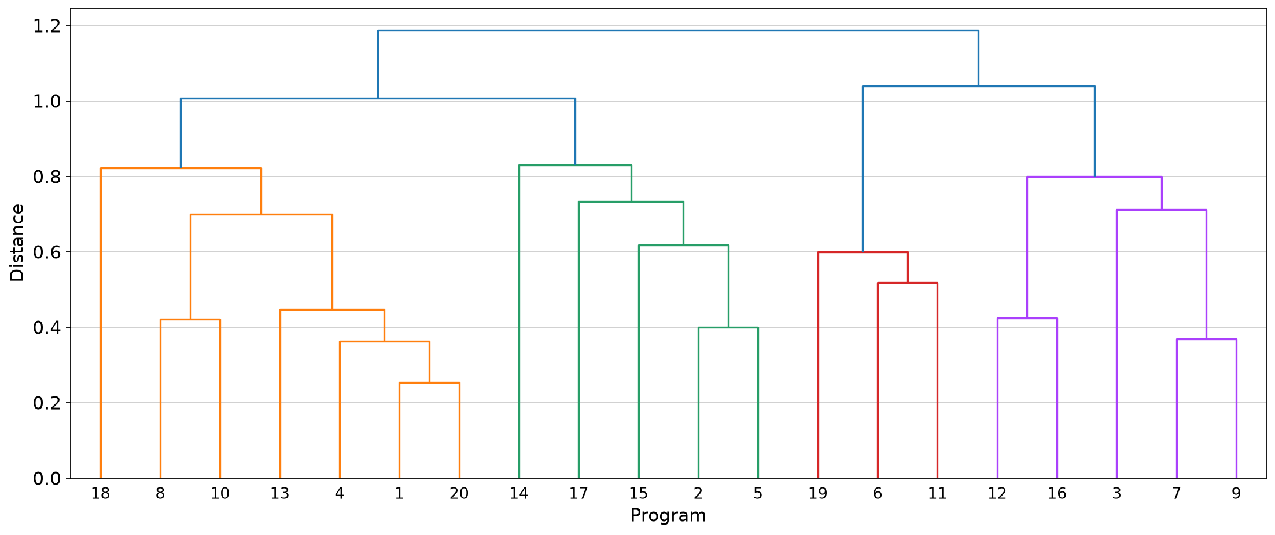
\includegraphics[width=1\textwidth]{img/dendogram.pdf}
	\caption{Program clustering based on relative responses to perturbations.}
	\label{fig:dendogram}
\end{figure}



%To characterize the effects of the perturbations on the inferred transcriptional programs, relative responses were examined across the perturbation set. 
%
%The relative response of an inferred transcriptional program quantifies the change in its inferred activity associated with a perturbation relative to the control reference. Positive values indicate a higher program response in the perturbed sample relative to the corresponding control, whereas negative values indicate a lower response. The magnitude of the value reflects the strength of the relative response on the scale produced by the D-SPIN analysis. These scores therefore provide a program-level measure of perturbation-associated changes and should not be interpreted as absolute expression levels or as direct measurements of gene regulatory activity.
%
%For each perturbation, programs were ranked according to their relative-response score, providing a measure of which transcriptional programs showed the strongest positive or negative changes relative to the control reference. The complete perturbation--program response matrix is shown in Figure \ref{fig:relative_responses}.
%
%\begin{figure}[h]
%	\centering
%	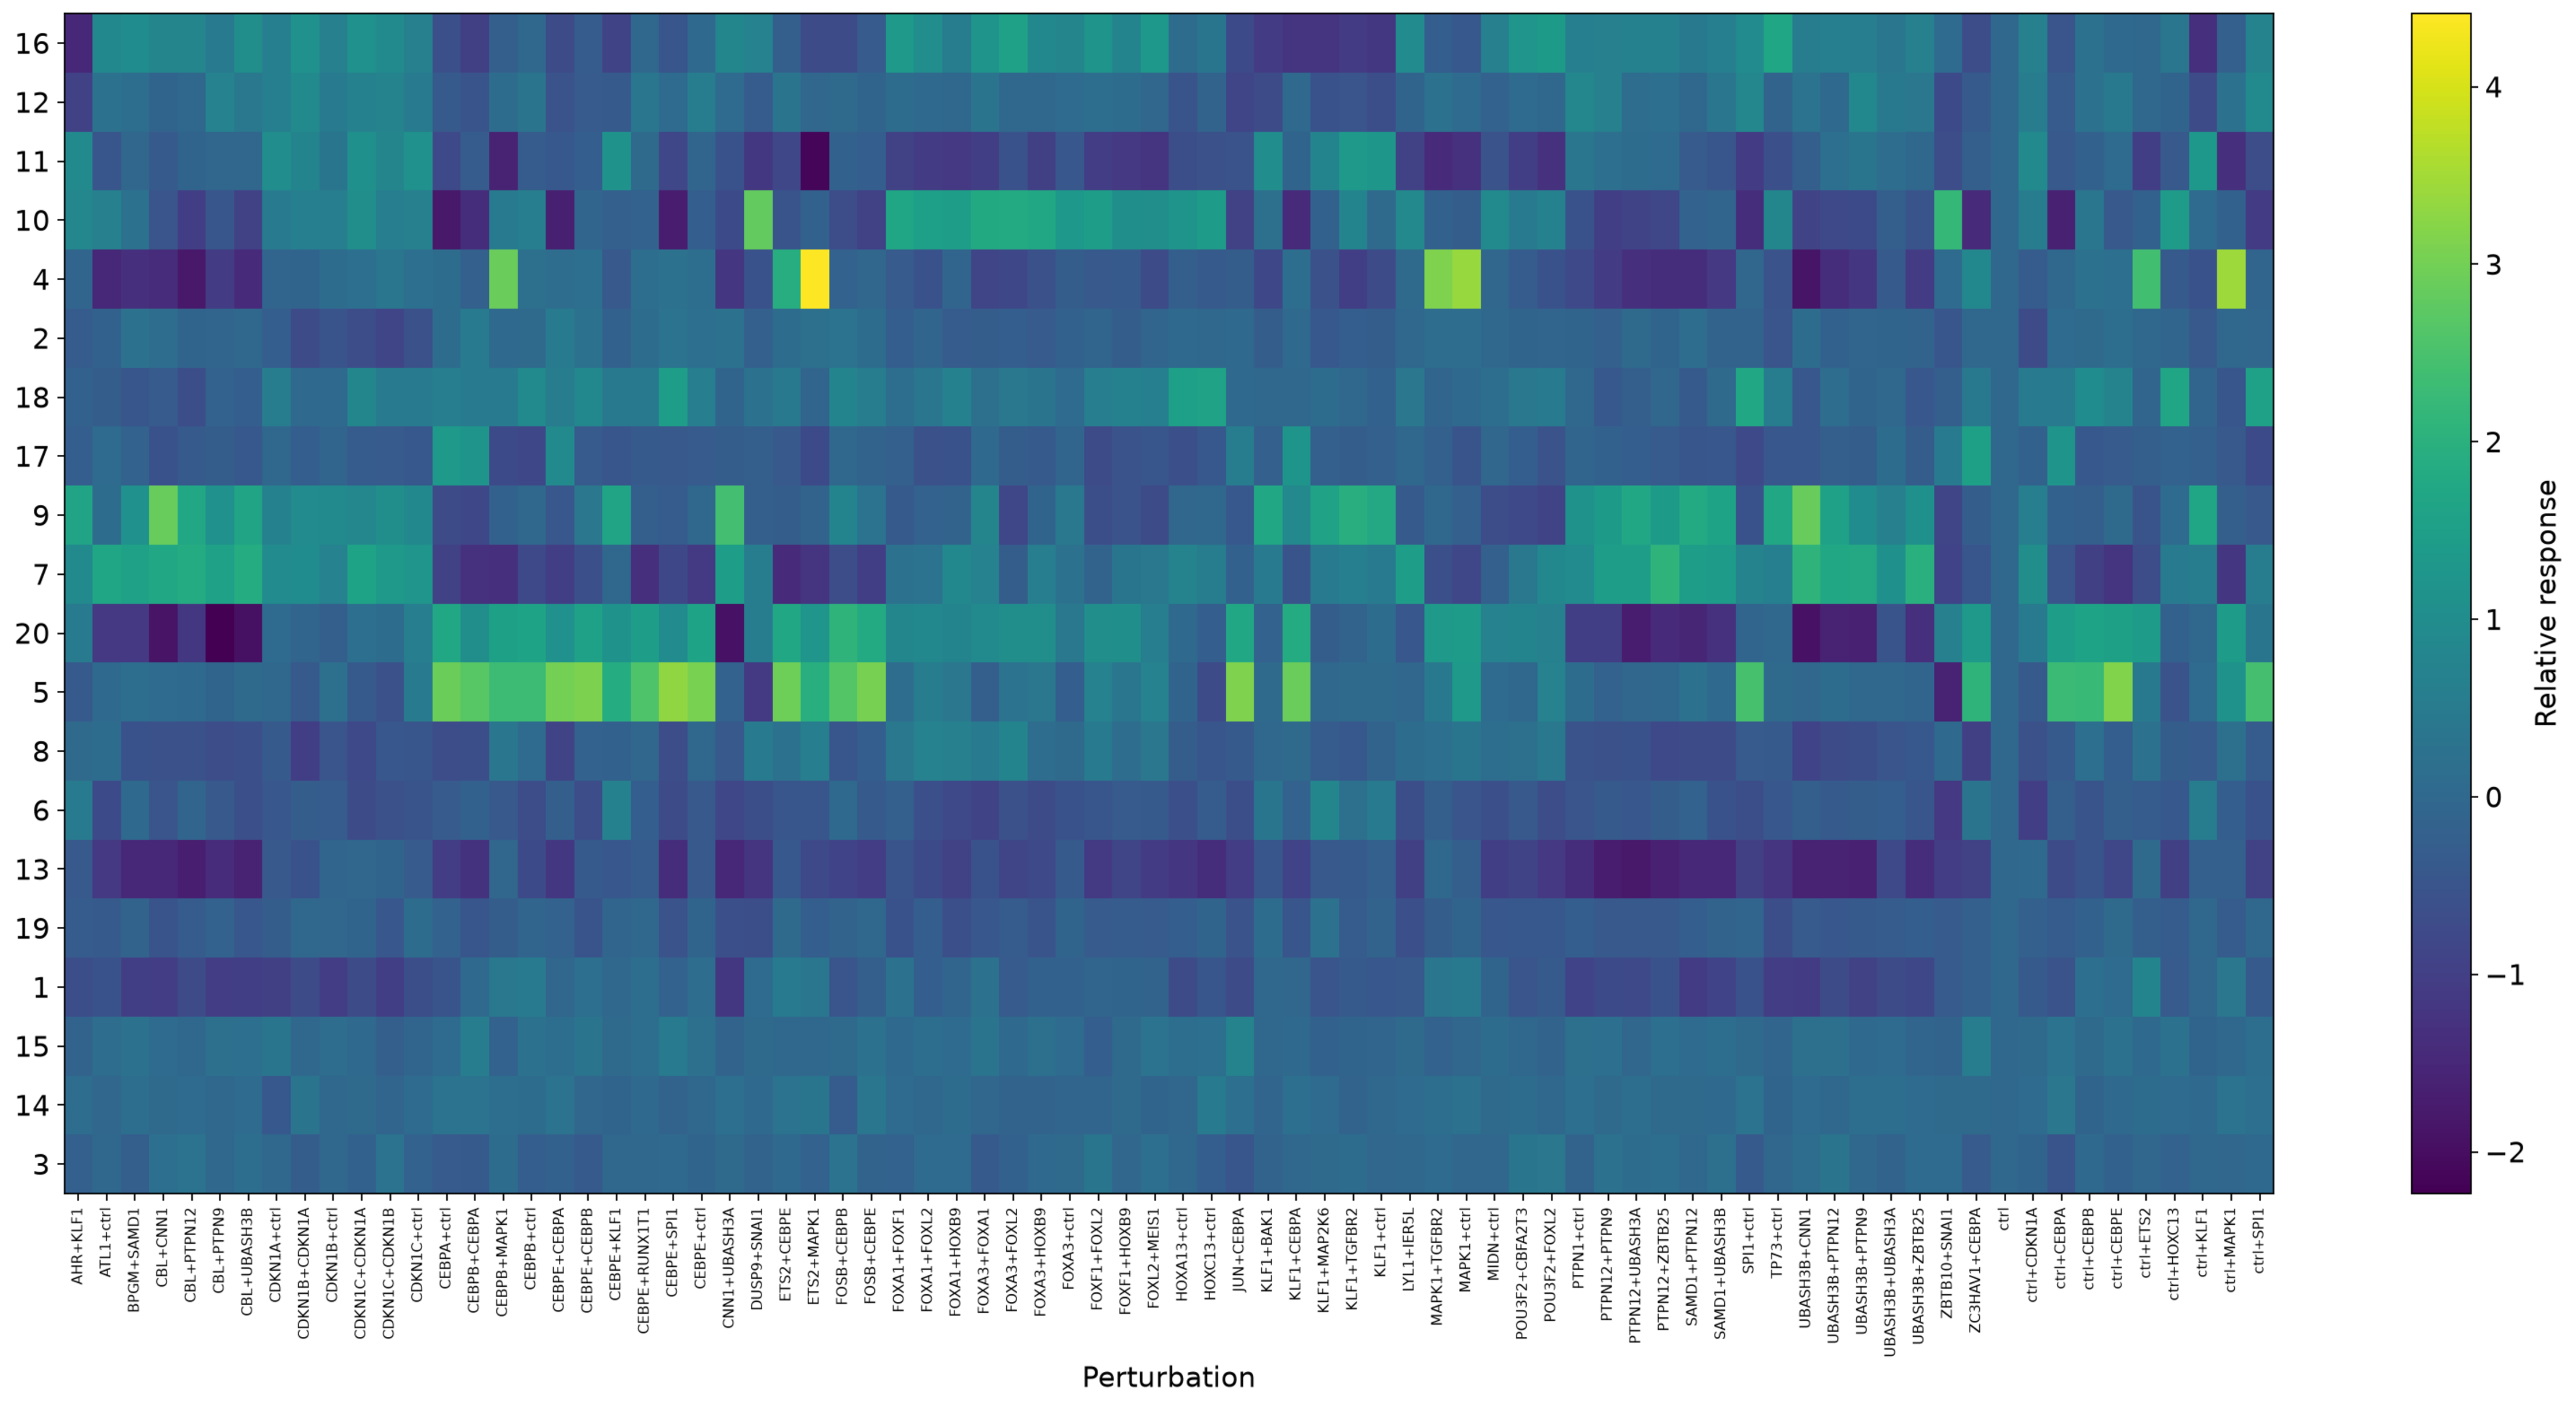
\includegraphics[width=1\textwidth]{img/relative_responses.pdf}
%	\caption{Relative responses of the inferred transcriptional programs to perturbations, with programs grouped according to enrichment analysis. Each column represents a perturbation and each row an inferred program. Positive values indicate increased relative program activity, whereas negative values indicate decreased relative activity.}
%	\label{fig:relative_responses}
%\end{figure}
%
%The distribution of responses across perturbations was heterogeneous, with several programs showing recurrent positive responses and others being activated only by specific perturbations. \textbf{Program 5} showed the highest mean relative response ($\mu = 0.79$) and was positive in 55 perturbations. Its strongest responses were observed for \textbf{CEBPE+SPI1} (3.30), \textbf{ctrl+CEBPE} (3.15), and \textbf{JUN+CEBPA} (3.14). Program 5 was also strongly associated with several additional CEBP-containing perturbations, including CEBPE+CEBPA (3.03), CEBPE+CEBPB (3.11), CEBPB+CEBPA (2.69), and CEBPB+ctrl (2.33). This recurrent pattern identifies Program 5 as one of the most broadly responsive programs in the perturbation dataset.
%
%\textbf{Program 9} showed the second-highest mean relative response ($\mu = 0.48$) and was positive in 43 perturbations. Its strongest responses were observed for \textbf{CBL+CNN1} (2.87), \textbf{UBASH3B+CNN1} (2.85), and \textbf{CNN1+UBASH3A} (2.43). Program 7 showed a related pattern, with positive responses in 49 perturbations and a maximum response of 2.08 for \textbf{UBASH3B+CNN1}. Other strong Program 7 responses were observed for PTPN12+ZBTB25 (2.08) and UBASH3B+ZBTB25 (1.98). Thus, perturbations involving CBL, UBASH3B, PTPN12, and CNN1 frequently produced high relative responses in Programs 7 and 9.
%
%A distinct response pattern was observed for perturbations involving \textbf{MAPK1} and \textbf{ETS2}. \textbf{Program 4} showed the largest individual relative-response value in the dataset, reaching 4.41 for \textbf{ETS2+MAPK1}. Strong Program 4 responses were also observed for ctrl+MAPK1 (3.45), MAPK1+ctrl (3.38), and MAPK1+TGFBR2 (3.13). Although Program 4 therefore showed the strongest individual responses, its mean response across perturbations was negative ($\mu = -0.13$), and it was positive in only 24 perturbations. This indicates that its high overall response was concentrated in a relatively restricted subset of perturbations rather than being broadly distributed across the dataset.
%
%Similarly, \textbf{Program 10} showed a relatively heterogeneous response distribution. Its maximum response was observed for \textbf{DUSP9+SNAI1} (2.80), followed by ZBTB10+SNAI1 (2.20) and FOXA3+FOXL2 (1.84). Program 10 was positive in 37 perturbations, with a mean response of 0.10. The selectivity analysis further emphasized the specificity of the SNAI1-associated responses: DUSP9+SNAI1 showed a Program 10 score of 2.80 compared with 0.70 for its second-ranked program, Program 16, while ZBTB10+SNAI1 showed a corresponding difference between Program 10 (2.20) and Program 20 (0.66).
%
%Several other programs showed recurrent but less selective responses. \textbf{Program 18} was positive in 51 perturbations and reached its highest value for \textbf{SPI1+ctrl} (1.75), followed by ctrl+HOXC13 (1.68) and HOXC13+ctrl (1.59). \textbf{Program 16} was positive in 52 perturbations, with its strongest responses observed for \textbf{TP73+ctrl} (1.70), FOXA3+FOXL2 (1.56), and POU3F2+FOXL2 (1.39). \textbf{Program 20} was positive in 49 perturbations and reached its highest response for \textbf{FOSB+CEBPB} (2.08), followed by KLF1+CEBPA (1.84) and FOSB+CEBPE (1.84). In contrast, Programs 13 and 19 showed relatively limited positive responses. Program 13 was positive in only two perturbations and had a mean relative response of $-0.85$, while Program 19 was positive in six perturbations and had a mean response of $-0.26$.
%
%The selectivity analysis showed that some perturbations produced strongly concentrated responses in a single program. The largest separation between the top-ranked and second-ranked programs was observed for \textbf{ETS2+MAPK1}, where Program 4 reached 4.41 compared with 1.96 for Program 5, giving a difference of 2.45. This was followed by \textbf{DUSP9+SNAI1}, with Program 10 at 2.80 versus Program 16 at 0.70, and by the MAPK1 control-orientation perturbations, ctrl+MAPK1 and MAPK1+ctrl, where Program 4 exceeded Program 20 by 2.01 and 1.98, respectively. CEBPE-associated perturbations also showed strong selectivity, with Program 5 exceeding Program 20 by 1.90 for CEBPE+CEBPA and by 1.84 for CEBPE+SPI1. These profiles indicate that, for a subset of perturbations, one inferred program accounted for a substantially larger relative response than the remaining programs.
%
%The reciprocal perturbation analysis provided an additional measure of the reproducibility of single-perturbation responses represented in the two possible orientations. All eight reciprocal pairs showed positive correlations, ranging from 0.84 for CDKN1A+ctrl versus ctrl+CDKN1A to 0.99 for SPI1+ctrl versus ctrl+SPI1. The highest correlations were observed for SPI1 ($r=0.985$), CEBPE ($r=0.987$), MAPK1 ($r=0.984$), KLF1 ($r=0.981$), and CEBPA ($r=0.980$). The corresponding RMSE values ranged from 0.13 for KLF1 to 0.30 for CDKN1A. Thus, although the exact response magnitudes were not identical between reciprocal representations, the overall program-response profiles were highly concordant for most perturbations.
%
%Overall, the relative-response analysis revealed distinct patterns of perturbation-associated program activity. Program 5 showed the broadest positive response across the perturbation set, particularly among CEBP-associated perturbations, whereas Programs 7 and 9 were repeatedly prominent among CBL-, PTPN12-, UBASH3B-, and CNN1-containing perturbations. Program 4 and Program 10 displayed particularly strong responses for specific perturbation combinations, with ETS2+MAPK1 and DUSP9+SNAI1 showing the strongest program selectivity. Other programs, including Programs 16, 18, and 20, exhibited recurrent positive responses across multiple perturbation classes. Conversely, Programs 13 and 19 were predominantly associated with negative or weak responses. The high concordance of reciprocal perturbation profiles further supports the consistency of the inferred program responses across alternative representations of single perturbations.
%
%These relative responses represent associations between perturbations and inferred program activity and should not be interpreted as evidence of direct regulatory interactions. In particular, a large relative-response value identifies a strong change in the corresponding inferred program but does not by itself establish which individual genes or regulatory mechanisms mediate that response.
%
%%\begin{table}[htbp]
%%	\centering
%%	\smaller[1]
%%	\renewcommand{\arraystretch}{1.2}
%%	\resizebox{\textwidth}{!}{%
%%		\begin{tabular*}{\linewidth}{@{\extracolsep{\fill}} cccc ccc }
%%			\hline
%%			\textbf{Program} & \textbf{Top response 1} & \textbf{Top response 2} & \textbf{Top response 3} &
%%			\textbf{Mean response} & \textbf{SD} & \textbf{N positive} \
%%			\hline
%%			1  & ctrl+ETS2 (0.7657) & CEBPB+ctrl (0.5168) & ETS2+CEBPE (0.4836) & -0.3453 & 0.4692 & 19 \
%%			2  & CEBPE+CEBPA (0.5327) & CEBPB+CEBPA (0.5023) & FOSB+CEBPB (0.3007) & -0.0840 & 0.2603 & 31 \
%%			3  & POU3F2+FOXL2 (0.3877) & POU3F2+CBFA2T3 (0.3601) & FOXF1+FOXL2 (0.3579) & -0.0218 & 0.1930 & 37 \
%%			4  & ETS2+MAPK1 (4.4116) & ctrl+MAPK1 (3.4472) & MAPK1+ctrl (3.3823) & -0.1331 & 1.1839 & 24 \
%%			5  & CEBPE+SPI1 (3.3028) & ctrl+CEBPE (3.1515) & JUN+CEBPA (3.1377) & 0.7873 & 1.2674 & 55 \
%%			6  & KLF1+MAP2K6 (0.8133) & CEBPE+KLF1 (0.6938) & ctrl+KLF1 (0.5691) & -0.3480 & 0.3649 & 10 \
%%			7  & UBASH3B+CNN1 (2.0836) & PTPN12+ZBTB25 (2.0787) & UBASH3B+ZBTB25 (1.9772) & 0.3836 & 1.0169 & 49 \
%%			8  & FOXA3+FOXL2 (0.7547) & FOXA1+FOXL2 (0.7146) & FOXA1+HOXB9 (0.6534) & -0.1903 & 0.4412 & 29 \
%%			9  & CBL+CNN1 (2.8713) & UBASH3B+CNN1 (2.8543) & CNN1+UBASH3A (2.4281) & 0.4826 & 0.9597 & 43 \
%%			10 & DUSP9+SNAI1 (2.8047) & ZBTB10+SNAI1 (2.2042) & FOXA3+FOXL2 (1.8375) & 0.1028 & 1.0250 & 37 \
%%			11 & KLF1+TGFBR2 (1.3622) & ctrl+KLF1 (1.2986) & KLF1+ctrl (1.2732) & -0.2596 & 0.7662 & 23 \
%%			12 & CDKN1B+CDKN1A (0.9335) & ctrl+SPI1 (0.9255) & UBASH3B+PTPN9 (0.8604) & 0.0818 & 0.4323 & 47 \
%%			13 & ctrl+ETS2 (0.0718) & ctrl+CDKN1A (0.0434) & ctrl (0.0000) & -0.8484 & 0.5095 & 2 \
%%			14 & HOXC13+ctrl (0.5149) & ctrl+CEBPA (0.4045) & FOSB+CEBPE (0.3799) & 0.0778 & 0.1551 & 53 \
%%			15 & JUN+CEBPA (0.7405) & CEBPB+CEBPA (0.5811) & ZC3HAV1+CEBPA (0.5447) & 0.1024 & 0.1787 & 55 \
%%			16 & TP73+ctrl (1.7040) & FOXA3+FOXL2 (1.5630) & POU3F2+FOXL2 (1.3863) & 0.2708 & 0.7792 & 52 \
%%			17 & ZC3HAV1+CEBPA (1.5472) & CEBPA+ctrl (1.3583) & CEBPB+CEBPA (1.2143) & -0.1744 & 0.4808 & 12 \
%%			18 & SPI1+ctrl (1.7518) & ctrl+HOXC13 (1.6760) & HOXC13+ctrl (1.5861) & 0.3061 & 0.5298 & 51 \
%%			19 & KLF1+MAP2K6 (0.2452) & CDKN1C+ctrl (0.1253) & KLF1+BAK1 (0.1220) & -0.2596 & 0.1986 & 6 \
%%			20 & FOSB+CEBPB (2.0790) & KLF1+CEBPA (1.8429) & FOSB+CEBPE (1.8379) & 0.2874 & 1.1542 & 49 \
%%			\hline
%%		\end{tabular*}%
%%	}
%%	\caption{Summary of relative responses for the inferred transcriptional programs. For each program, the three perturbations with the highest relative-response scores are shown together with their scores. Mean response, standard deviation (SD), and the number of perturbations with a positive response are also reported.}
%%	\label{tab:program_relative_response_summary}
%%\end{table}

\newpage 

\subsection{Directional network}

To further investigate the organization of the inferred transcriptional programs, a directed network was constructed from the program-level interaction matrix estimated by D-SPIN. Whereas the preceding correlation analyses describe statistical relationships between program activity or relative-response profiles, the D-SPIN network represents the inferred interactions between program states within the probabilistic model. The network therefore provides a complementary representation of how the inferred programs may be organized through positive and negative interactions under the different perturbation conditions. In the D-SPIN formulation, positive interaction weights favor programs adopting the same state, whereas negative interaction weights favor different states. Consequently, positive and negative edges should be interpreted as inferred program-level interaction signs rather than as direct evidence of transcription-factor binding or biochemical regulation \cite{Jiang2023}.

The network was visualized using the directed-network representation provided by D-SPIN. Interactions with an absolute strength below $0.05$ were removed during network construction, while a directional asymmetry threshold of $0.05$ was used to distinguish preferentially directed interactions from approximately symmetric interactions. For visualization, only interactions with an absolute weight of at least $0.25$ were displayed. Modules were identified by Leiden clustering with a resolution parameter of $1.0$. The resulting network contained four modules, with sizes of 7, 6, 4, and 3 programs, respectively. The resulting partition was stable with respect to the random seed used for the Leiden procedure, as identical module assignments were obtained across all tested seeds.

The inferred modular organization was also relatively robust to the choice of directional threshold. Increasing the directional threshold from $0.05$ to $0.10$ and $0.20$ changed the classification of several individual edges from directed to approximately reciprocal, but did not alter the membership of the four modules. This indicates that the higher-level modular organization was not dependent on the precise value used to define directional asymmetry. The resolution parameter affected the finer partitioning of the network. Resolutions of $0.5$ and $0.75$ also produced four modules, whereas resolutions of $1.25$ and above produced five modules. Thus, the four-module organization observed at the selected resolution represents a stable coarse-grained structure of the inferred network, while some individual program assignments depend on the clustering resolution.


\begin{figure}[h]
	\centering
	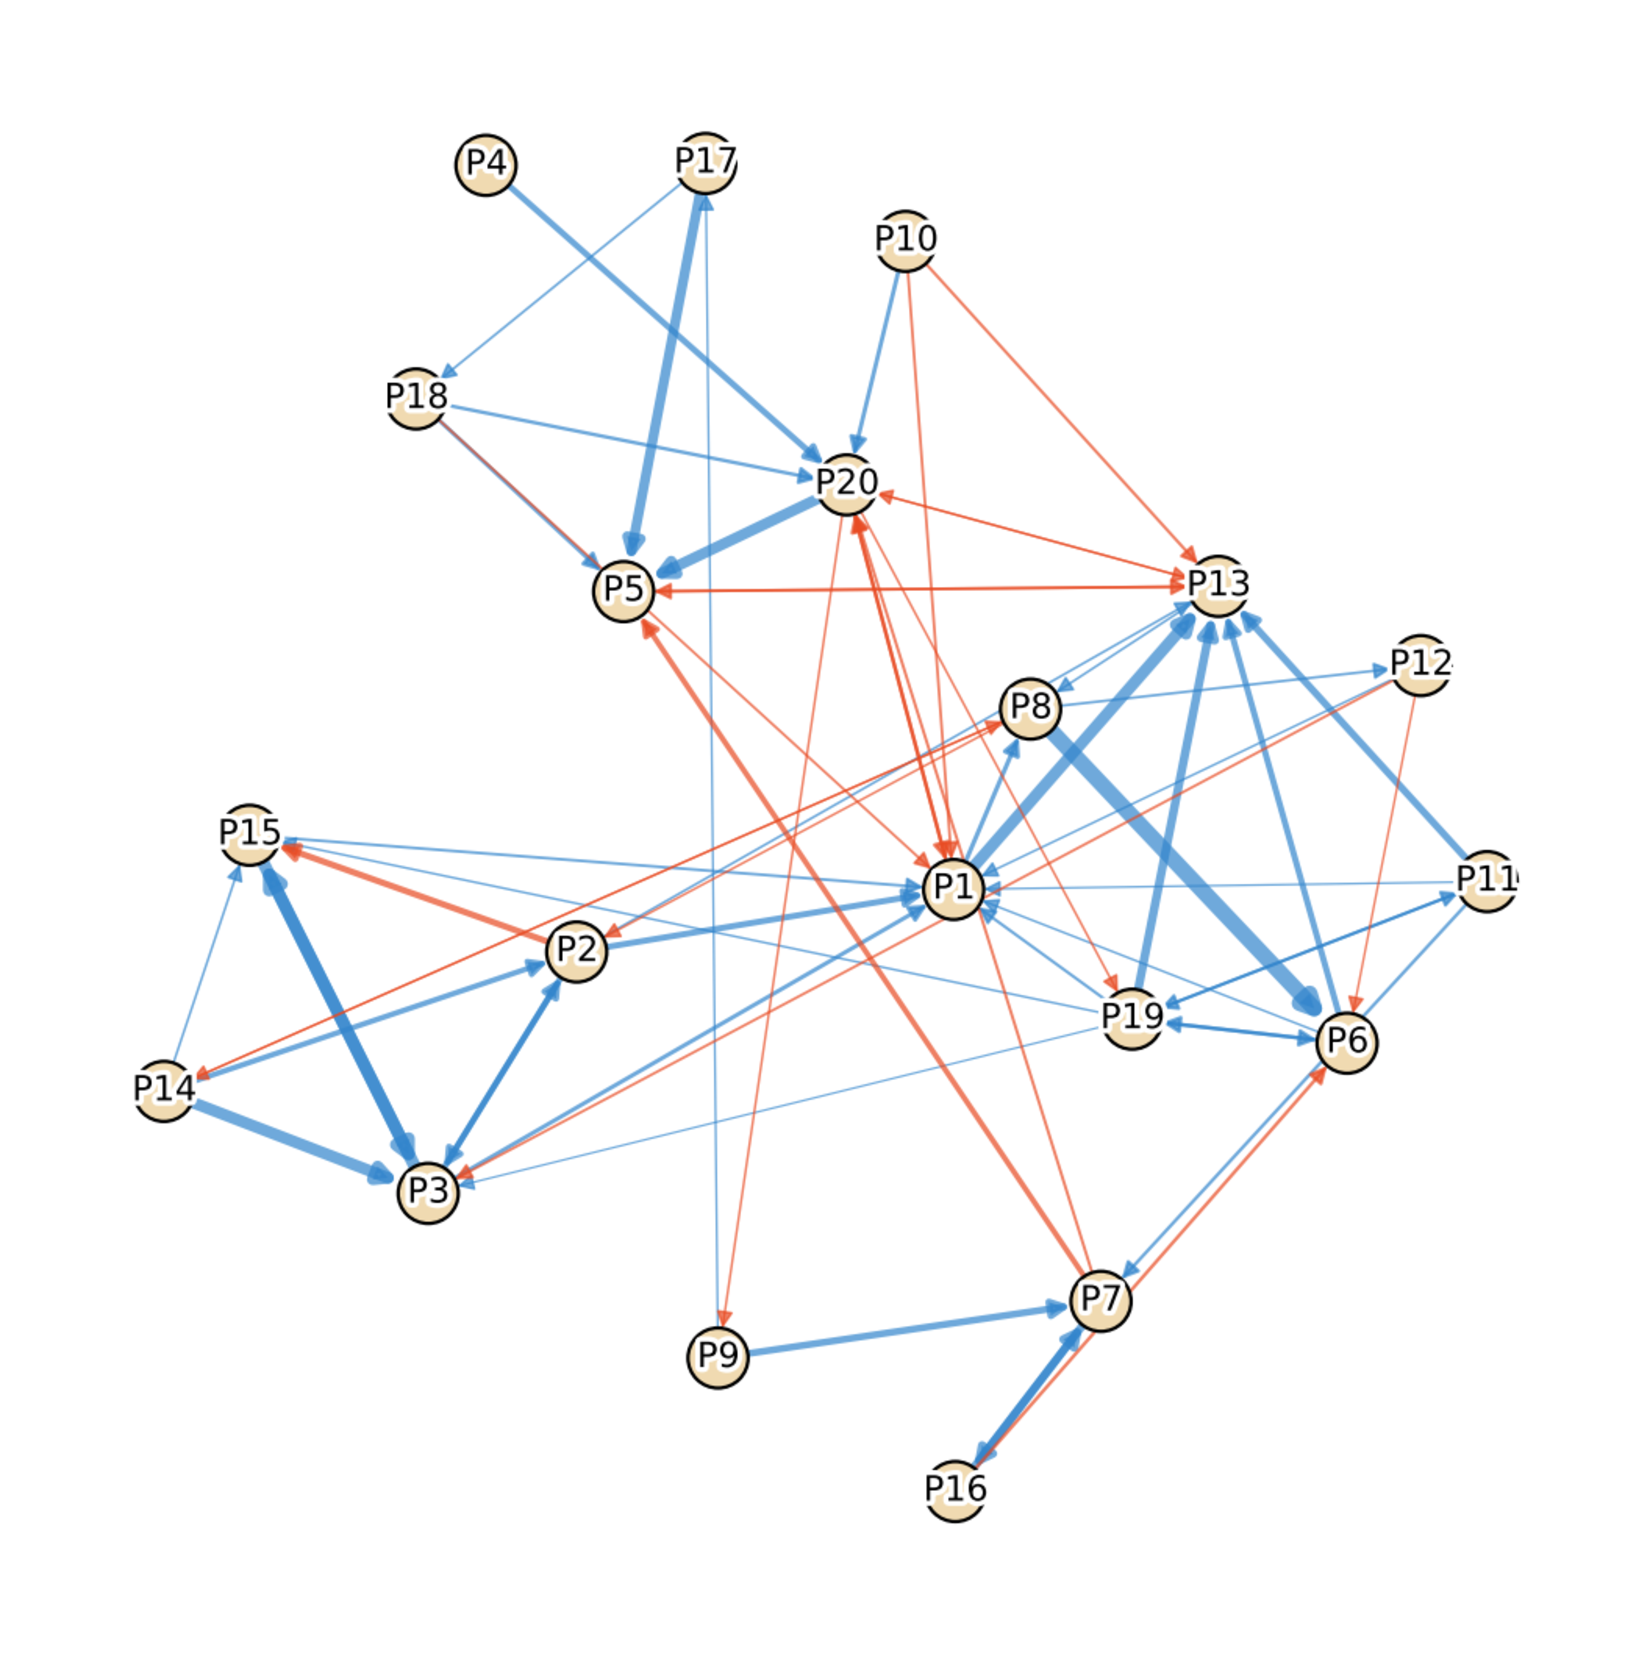
\includegraphics[width=0.7\textwidth]{img/network.pdf}
	\caption{Program network constructed by DSPIN. }
	\label{fig:network}
\end{figure}


The network showed a pronounced organization of strong positive interactions within modules. Several of the strongest positive edges connected programs belonging to the same inferred module. In particular, strong positive interactions were observed from Program 8 to Program 6, from Program 13 to Program 1, from Program 20 to Program 5, from Program 4 to Program 20, from Program 3 to Program 15, from Program 14 to Program 3, and from Program 16 to Program 7. These interactions link programs within the corresponding modules rather than connecting different modules. Additional positive edges with substantial weight included the interactions from Program 9 to Program 7, Program 13 to Program 6, Program 19 to Program 13, Program 6 to Program 13, Program 10 to Program 20, Program 18 to Program 20, Program 18 to Program 5, and Program 17 to Program 5. Together, these connections indicate that the modules are characterized by dense positive reinforcement or coordination among their member programs.

The first module comprised Programs 13, 1, 6, 19, 8, 12, and 11. Several of the strongest interactions in the complete network were located within this group. In particular, Program 13 showed strong positive connections to Programs 1 and 6, while reciprocal positive relationships were present between Programs 19 and 13 and between Programs 6 and 13. Program 8 was also strongly connected to Program 6. Additional weaker positive interactions connected Program 19 to Programs 11 and 6, Program 8 to Programs 19 and 12, and Program 12 to Program 1. The overall pattern therefore suggests a highly interconnected positive subnetwork, in which several programs exhibit mutually reinforcing or coordinated interaction weights. The presence of multiple positive edges within the same module is consistent with the module being a coherent component of the inferred network.

The second module consisted of Programs 5, 20, 17, 10, 4, and 18. This module contained several strong positive interactions centered on Programs 5 and 20. Program 4 was positively connected to Program 20, while Program 18 showed positive connections to both Programs 20 and 5. Program 17 was also positively connected to Program 5. Program 10 showed a positive interaction with Program 20, and Program 17 was positively connected to Program 20. The resulting structure indicates that these programs form a closely connected positive subnetwork. In addition, a weaker positive interaction linked Program 17 to Program 18, providing further internal connectivity. The presence of several strong positive interactions within this module suggests that the programs grouped together by Leiden clustering are connected by relatively strong inferred network interactions.

The third module comprised Programs 3, 15, 2, and 14. This module was characterized by a particularly strong positive interaction chain involving Programs 14, 3, and 15. Program 14 showed a strong positive interaction with Program 3, while Program 3 showed a strong positive interaction with Program 15. Program 14 was also positively connected to Program 2. A further positive interaction was observed between Programs 15 and 3 in the opposite direction, producing a reciprocal relationship between these two programs. Together, these interactions define a compact positive subnetwork in which Programs 14, 3, and 15 occupy central positions. The strong internal connectivity of this small module distinguishes it from the larger modules and suggests that these programs form a tightly coordinated component of the inferred network.

The fourth module consisted of Programs 7, 16, and 9. This module was dominated by strong positive interactions involving Program 7. Program 16 showed a strong positive interaction with Program 7, and Program 9 was also positively connected to Program 7. A reciprocal interaction between Programs 7 and 16 was retained, indicating that the inferred relationship between these two programs was comparatively symmetric at the selected directional threshold. Additional weaker positive interactions connected Program 16 to Program 9 and Program 11 to Program 7. The compact organization of this module suggests a small program group centered around Program 7.

In contrast to the predominantly positive interactions within modules, many of the strongest negative interactions connected programs belonging to different modules. This pattern was particularly apparent for the negative edges shown in red in the network diagram. Strong negative interactions included Program 2 to Program 15, Program 7 to Program 5, Program 10 to Program 13, Program 10 to Program 5, Program 1 to Program 5, Program 1 to Program 7, Program 20 to Program 13, and Program 20 to Program 1. These interactions frequently linked programs belonging to distinct modules. For example, Program 10 is part of the second module, whereas Program 13 belongs to the first module, producing a negative interaction between these two modules. Similarly, the negative interaction from Program 7 to Program 5 links the fourth and second modules, while Program 1 to Program 7 connects the first and fourth modules.

The negative interactions therefore provide a complementary organization to the positive intra-module structure. Rather than simply representing isolated negative associations, many of the strongest negative edges form connections between otherwise positively organized modules. This pattern is consistent with a network architecture in which programs within a module tend to support coordinated states, whereas interactions between some modules favor contrasting program states. In the D-SPIN model, a negative interaction does not necessarily imply that one program directly represses another; rather, it indicates that the inferred network assigns a negative coupling between the two program states, such that simultaneous activation or simultaneous inhibition is less favored than differing states \cite{Jiang2023}.

Several additional negative interactions further illustrate this modular separation. Program 20 showed negative interactions with Programs 13 and 1, connecting the second module to the first. Program 20 also showed a negative interaction with Program 19, again linking the second and first modules. Program 18 exhibited both a strong positive interaction with Program 20 and a weaker negative interaction with the same program. This coexistence of positive and negative contributions emphasizes that the sign and direction of the interaction should be considered together with its magnitude rather than interpreted solely from the existence of an edge. Similarly, Programs 14 and 8 were connected by a weaker negative interaction despite being members of different modules, whereas Program 3 showed a weak negative interaction with Program 12, providing another example of cross-module opposition.

The network also contained a number of weaker positive edges that were retained in the inferred network but fell below the threshold used for the main network visualization. These included, among others, interactions from Program 17 to Program 18, Program 19 to Programs 11 and 6, Program 8 to Programs 19 and 12, Program 11 to Program 7, Program 12 to Program 1, Program 15 to Programs 14 and 3, Program 19 to Program 1, Program 3 to Program 2, Program 2 to Program 13, Program 6 to Program 19, and Program 1 to Program 17. Although these interactions were not emphasized in the main network figure because of the visualization threshold, their presence contributes to the overall connectivity of the inferred network and provides additional links both within and between modules.

An additional feature of the network is that some program pairs exhibited interactions in both directions. For example, positive reciprocal relationships were apparent between Programs 3 and 15, Programs 7 and 16, Programs 6 and 13, and Programs 13 and 19 under the displayed network structure. The occurrence of reciprocal interactions indicates that the inferred relationship between two programs cannot always be reduced to a single preferred direction. Conversely, several interactions were represented by a single directed edge because the inferred coupling was sufficiently asymmetric to satisfy the directional criterion. The distinction between directed and approximately symmetric interactions is therefore part of the network structure rather than simply a property of the visualization.

The sensitivity analysis further showed that the exact set of directional edges depends more strongly on the directional threshold than the module assignment does. At a directional threshold of $0.05$, most retained program pairs were classified as directional, whereas increasing the threshold to $0.10$, $0.20$, $0.30$, and $0.50$ progressively increased the number of interactions treated as approximately symmetric. Nevertheless, the module assignments remained unchanged between directional thresholds of $0.05$ and $0.20$. This indicates that some individual arrows should be interpreted with greater caution than the broader modular structure. In particular, the direction of relatively moderate interactions may depend on the asymmetry criterion, whereas the strongest network relationships and the overall grouping of programs are less sensitive to this parameter.

The interaction network therefore revealed two complementary levels of organization. At the local level, each module contained several positive interactions connecting its constituent programs, with some modules displaying particularly strong reciprocal or directed relationships. At the global level, negative interactions frequently connected programs belonging to different modules, suggesting antagonistic or contrasting organization between subsets of programs. The resulting structure is consistent with a network in which perturbation responses are not distributed independently across programs, but instead propagate through a limited number of coordinated program groups that interact positively within modules and oppose selected programs in other modules.

Importantly, the directionality of the inferred network should not be interpreted as direct evidence of causality between the corresponding transcriptional programs. D-SPIN infers a probabilistic interaction model that describes how program states are statistically coupled across the perturbation dataset. The directed representation captures asymmetry in the inferred interaction weights, but does not by itself establish a direct biochemical or transcriptional regulatory mechanism. Consequently, edges such as Program 8 $\rightarrow$ Program 6 or Program 13 $\rightarrow$ Program 1 are best interpreted as inferred directional dependencies within the D-SPIN network rather than as experimentally validated regulatory events.

Overall, the directional network provides a higher-level representation of the organization identified in the preceding perturbation-response analyses. The network separates the 20 programs into four principal modules and reveals strong positive interactions within these groups, together with negative interactions that frequently connect programs from different modules. The strongest positive connections are concentrated within modules, while several of the strongest negative interactions bridge modules, producing a structured pattern of coordination and opposition. The stability of the module assignments across directional thresholds and Leiden seeds further supports the presence of a reproducible modular organization, while the sensitivity of individual edge directions to the directional threshold indicates that specific directional relationships should be interpreted more cautiously. Together, these results suggest that the perturbation responses identified in the relative-response analysis are organized within a structured program network consisting of coordinated modules and contrasting inter-module interactions.


\newpage

\section{A final reachout}

%\subsection{Comparison with the original Norman et al. perturbational landscape}

\subsection{Comparison with the Norman et al. perturbational landscape}

The dataset analysed in this study originates from the CRISPRa Perturb-seq experiment reported by Norman et al.~\citep{Norman2019}. The original study used transcriptional phenotypes to characterize genetic interactions in K562 cells and identified several biologically interpretable perturbational groups. These groups include G1 cell cycle, Erythroid, Pioneer factors, Granulocyte apoptosis, Pro-growth, and Megakaryocyte programmes, which are also provided as perturbation annotations in the current \textcolor{red}{PertPy} representation of the Norman dataset \citep{Heumos2026}. These annotations provide an independent reference against which the D-SPIN relative-response profiles can be interpreted.

The comparison does not represent a direct replication of the Norman et al.~analysis. The two approaches organize the same transcriptional dataset differently. Norman et al.~primarily organized perturbations according to their genome-wide transcriptional phenotypes, whereas D-SPIN decomposes the transcriptional measurements into latent programs and then estimates a relative response for each program and perturbation. Consequently, one biological perturbational programme may be represented by several D-SPIN programs, and individual D-SPIN programs need not correspond one-to-one to a single Norman category. The comparison therefore focuses on whether the major biological response classes identified in the original study are also reflected in the D-SPIN program composition and relative-response profiles.

\subsubsection{Quantitative comparison of D-SPIN programs with Norman perturbation groups}

To compare the two representations, the relative-response values were grouped according to the perturbational programmes defined for the Norman dataset. For each D-SPIN program and Norman category, the mean relative response was calculated across the perturbations assigned to that category. When a single-gene perturbation was represented in the D-SPIN dataset as either a gene+ctrl or ctrl+gene condition, only one orientation was used for the category-level summary to avoid counting the same biological perturbation twice.

The strongest correspondences are summarized in Table~\ref{tab:dspin_norman_comparison}. Several D-SPIN programs showed markedly positive mean responses within biologically coherent Norman categories, indicating that the perturbational structure described in the original study is recovered in the D-SPIN response space.

\begin{table}[htbp]
	\centering
	\renewcommand{\arraystretch}{1.2}
	\setlength{\tabcolsep}{6pt}
	\begin{tabular*}{\linewidth}{@{\extracolsep{\fill}} l l c c c}
		\hline
		\textbf{Program} & \textbf{Norman programme} & \textbf{Mean response} & \textbf{Minimum} & \textbf{Maximum} \\
		\hline
		Program 7  & Erythroid               & 1.631 & 0.963 & 2.084 \\
		Program 9  & Erythroid               & 1.605 & 0.660 & 2.871 \\
		Program 5  & Granulocyte apoptosis   & 2.818 & 2.100 & 3.303 \\
		Program 20 & Granulocyte apoptosis   & 1.477 & 0.337 & 2.079 \\
		Program 4  & Megakaryocyte            & 3.243 & 2.390 & 4.412 \\
		Program 10 & Pioneer factors          & 1.442 & 0.687 & 2.805 \\
		\hline
	\end{tabular*}
	\caption{Mean D-SPIN relative responses for selected programs across perturbations belonging to the corresponding Norman et al.~programmes. Minimum and maximum values indicate the range of relative responses within each category. The number of perturbations contributing to each summary was 17 for Erythroid, 15 for Granulocyte apoptosis, 5 for Megakaryocyte, and 18 for Pioneer factors.}
	\label{tab:dspin_norman_comparison}
\end{table}

\subsubsection{Erythroid response}

The strongest correspondence with the erythroid perturbational programme was observed for \textbf{Programs 7 and 9}. Program 7 was characterized by GYPA, GYPB, and HBG2 among its three highest-weight genes and showed enrichment for oxygen, carbon dioxide, and gas-transport processes. Program 9 was similarly characterized by HBA1, HBA2, and HEMGN. Thus, the gene composition of both programs provided independent evidence for erythroid-related transcriptional states.

The relative-response profiles provided a second and independent line of evidence. Across the 17 perturbations assigned to the Norman erythroid programme, Program 7 had a mean relative response of $1.631$, with responses ranging from $0.963$ to $2.084$. Program 9 showed a mean response of $1.605$, ranging from $0.660$ to $2.871$. Both programs therefore exhibited consistently positive responses across the erythroid-associated perturbation set rather than being driven by a single perturbation.

The strongest individual response was observed for CBL+CNN1, for which Program 9 reached $2.8713$ and Program 7 reached $1.7399$. Program 7 also reached $1.8762$ for CBL+UBASH3B, while Program 9 reached $1.6552$ for the same perturbation. For UBASH3B+CNN1, the corresponding responses were $2.0836$ for Program 7 and $2.8543$ for Program 9. These repeated responses indicate that the two programs are consistently associated with the same perturbational region of the dataset.

This agreement is particularly relevant because Norman et al.~identified CBL+CNN1 as a strong genetic interaction associated with an erythroid phenotype \citep{Norman2019}. The D-SPIN results therefore reproduce this biological association at the level of latent program activity: perturbations previously characterized as erythroid-associated generate strong responses in programs whose gene composition is independently consistent with erythroid differentiation.

The coordinated behavior of Programs 7 and 9 is further supported by their relative-response correlation of $r=0.63$. Thus, the erythroid phenotype is not represented by a single isolated D-SPIN program, but by at least two programs whose responses tend to vary together across perturbations. This is consistent with the decomposition of a broad cellular phenotype into multiple transcriptional components.

Program 16 provides a further possible erythroid-related component. ALAS2 was its highest-weight gene, and the program showed positive relative responses to several perturbations associated with erythroid differentiation. Its correspondence with the Norman erythroid programme was, however, less specific than those of Programs 7 and 9 and is therefore interpreted more cautiously.

\subsubsection{Granulocyte-associated response}

A second strong correspondence was observed for \textbf{Program 5}. Its highest-weight genes were LST1, TYROBP, and CSF3R, and its functional enrichment was associated with hematopoietic and immune-related processes. These features are consistent with a myeloid/granulocytic transcriptional state.

The perturbation-level evidence was particularly strong. Across the 15 perturbations assigned to the Norman Granulocyte apoptosis programme, Program 5 had a mean relative response of $2.818$, with all values lying between $2.100$ and $3.303$. This was substantially higher than the mean response observed for most other programs in the same perturbation set. Strong responses were observed for CEBPE+SPI1 ($3.3028$), CEBPE+ctrl ($3.0866$), CEBPE+CEBPB ($3.1081$), CEBPE+CEBPA ($3.0262$), CEBPE+RUNX1T1 ($2.5841$), CEBPA+ctrl ($2.9151$), KLF1+CEBPA ($2.8837$), and JUN+CEBPA ($3.1377$).

This pattern closely follows the perturbation composition of the Norman Granulocyte apoptosis programme, which includes SPI1, CEBPA, CEBPB, CEBPE, and several combinations involving these factors \citep{Norman2019,Heumos2026}. The agreement between the program gene signature and its perturbational response therefore provides convergent evidence for a granulocyte-associated interpretation of Program 5.

Program 20 also showed a positive response across this perturbational group, with a mean relative response of $1.477$. Its responses ranged from $0.337$ to $2.079$, and particularly strong responses were observed for FOSB+CEBPB ($2.0790$), FOSB+CEBPE ($1.8379$), KLF1+CEBPA ($1.8429$), and JUN+CEBPA ($1.7507$). The positive correlation between Programs 5 and 20 ($r=0.63$) is therefore consistent with their recurrent co-occurrence in CEBP- and related perturbations.

The relationship between the erythroid and granulocyte-associated programs is particularly apparent from the negative relative-response correlation between Programs 7 and 20 ($r=-0.87$). Programs 7 and 20 therefore represent contrasting perturbational response patterns: the former is strongly activated by the erythroid-associated CBL/UBASH3B/PTPN12-related perturbations, whereas the latter is more prominent among CEBP- and FOSB-associated perturbations. The strong negative correlation provides a quantitative indication that these biological response classes occupy opposing regions of the D-SPIN relative-response space.

\subsubsection{Megakaryocyte-associated response}

\textbf{Program 4} provided a particularly informative comparison because its gene-level annotation was inconclusive. No significant Gene Ontology Biological Process terms were detected for this program, and its top genes did not provide an unambiguous functional interpretation. In contrast, its perturbation-response profile showed a strong and highly selective association with the Norman Megakaryocyte programme.

Across the five perturbations assigned to this category, Program 4 had a mean relative response of $3.243$, with values ranging from $2.390$ to $4.412$. The strongest response occurred for ETS2+MAPK1 ($4.4116$), followed by MAPK1+ctrl ($3.3823$), MAPK1+TGFBR2 ($3.1298$), CEBPB+MAPK1 ($2.9024$), and ctrl+ETS2 ($2.3901$). The concentration of the strongest responses in MAPK1- and ETS2-containing perturbations is highly consistent with the Megakaryocyte programme defined for the Norman dataset, which includes MAPK1, ETS2, ETS2+MAPK1, MAPK1+TGFBR2, and CEBPB+MAPK1 \citep{Norman2019,Heumos2026}.

This example demonstrates that perturbation-response analysis can provide biological information that is not apparent from gene-set enrichment alone. Program 4 could not be assigned confidently on the basis of its GO enrichment, whereas its response to a predefined perturbational category provides a much clearer biological interpretation.

\subsubsection{Pioneer-factor response}

The same approach identified a broader response pattern associated with the \textbf{Pioneer factors} category. Program 10 showed particularly strong responses to the perturbations belonging to this group. Across the 18 annotated pioneer-factor perturbations represented in the present matrix, Program 10 had a mean relative response of approximately $1.442$, with values ranging from $0.687$ to $2.805$.

The strongest response was observed for DUSP9+SNAI1 ($2.8047$), followed by ZBTB10+SNAI1 ($2.2042$). Program 10 also showed strong responses across multiple FOXA-associated perturbations, including FOXA1+FOXF1 ($1.6619$), FOXA1+FOXL2 ($1.5196$), FOXA1+HOXB9 ($1.4815$), FOXA3+FOXA1 ($1.8027$), FOXA3+FOXL2 ($1.8375$), FOXA3+HOXB9 ($1.7578$), FOXF1+FOXL2 ($1.4901), and FOXF1+HOXB9 ($1.0674). This broad response profile suggests that Program 10 captures a transcriptional component associated with the pioneer-factor perturbations rather than being restricted to a single perturbation combination.

The perturbation-response analysis therefore extends the biological interpretation of Program 10 beyond its individual top genes. The recurrence of positive responses across different FOXA-, SNAI1-, HOXC13-, and related perturbations is consistent with a shared transcriptional response axis corresponding to the pioneer-factor programme defined in the original dataset.

\subsubsection{Cell-cycle response}

The Norman G1-cell-cycle category provides a somewhat different type of correspondence. The six annotated perturbations in this group comprise CDKN1A, CDKN1B, CDKN1C, and their pairwise combinations with each other. D-SPIN recovered several programs with positive responses to these perturbations, but no single program was uniquely associated with the entire G1 category.

For example, Program 11 had a mean relative response of approximately $0.860$ across the six G1 perturbations, while Program 16 showed a similar mean response of approximately $0.857$. Programs 7 and 9 also showed positive mean responses of approximately $1.144$ and $0.895$, respectively. The distribution across multiple programs suggests that the G1 perturbational state is represented by several transcriptional components rather than a single latent factor.

This observation is consistent with the biological composition of the D-SPIN programs. Program 2 was enriched for DNA replication, DNA repair, and DNA damage-response processes and contained HIST1H4C, KIAA0101, and TYMS. Program 3 contained CKS2, CENPF, and BIRC5 and was enriched for cell-cycle and mitotic chromosome-segregation processes. Programs 14 and 15 were similarly characterized by CDK1/PIF1/GTSE1 and PLK1/CDC20/CCNB1, respectively. These programs therefore capture different molecular components of proliferative and mitotic activity, even if their responses do not map one-to-one onto the Norman G1 perturbational category.

\subsubsection{Program-level representation of the Norman perturbational landscape}

The comparison suggests that the D-SPIN relative-response matrix preserves major biological distinctions originally identified by Norman et al.~while representing them at a different level of organization. The original study grouped perturbations according to their transcriptional phenotypes, whereas D-SPIN groups programs according to how their inferred activity responds across perturbations. The correspondence between the two representations is therefore expected to emerge as similar patterns of association rather than as identical clusters.

This relationship is particularly clear for the erythroid and granulocyte-associated perturbations. The CBL-, UBASH3B-, PTPN12-, PTPN9-, and CNN1-containing perturbations assigned to the Norman erythroid programme produced strong responses in Programs 7 and 9. Conversely, CEBPA-, CEBPB-, CEBPE-, SPI1-, FOSB-, and JUN-containing perturbations assigned to the Norman Granulocyte apoptosis programme produced strong responses in Program 5 and, to a lesser extent, Program 20. The separation between these two response classes is further reflected in the strong negative correlation between Programs 7 and 20.

The megakaryocyte category provides a second clear example. The five perturbations defined in the Norman Megakaryocyte programme produced an average relative response of $3.243$ in Program 4, considerably larger than the responses observed for most other perturbational categories. Thus, the MAPK1/ETS2 perturbational axis is recovered as a distinct D-SPIN response programme even though Program 4 could not be annotated confidently using GO enrichment alone.

The pioneer-factor category likewise demonstrates that D-SPIN captures a broader perturbational axis rather than merely isolated pairwise effects. Program 10 responded positively across a large number of FOXA-, HOX-, SNAI1-, TP73-, and related perturbations. This pattern indicates that the response is associated with a common perturbational programme spanning multiple transcriptional regulators.

Taken together, these results indicate that the D-SPIN programs recover several major biological axes already present in the original Norman dataset. The strongest correspondences are summarized by the following associations:

$$
\begin{aligned}
\text{Programs 7 and 9}
&\longleftrightarrow
\text{Erythroid perturbations},\\
\text{Programs 5 and 20}
&\longleftrightarrow
\text{Granulocyte-associated perturbations},\\
\text{Program 4}
&\longleftrightarrow
\text{Megakaryocyte perturbations},\\
\text{Program 10}
&\longleftrightarrow
\text{Pioneer-factor perturbations}.
\end{aligned}
$$

These correspondences are supported by multiple levels of evidence, including the genes defining the programs, Gene Ontology enrichment, the magnitude and recurrence of relative responses across perturbations, and the independent perturbational annotations established for the original dataset.

The comparison should nevertheless be interpreted as a concordance analysis rather than as a direct replication of the Norman et al.~results. The number, boundaries, and biological composition of D-SPIN programs are not expected to coincide exactly with the perturbational groups defined in the original study. Instead, the results indicate that the major biological response axes identified previously are retained within the D-SPIN representation and can be resolved into multiple coordinated transcriptional programs.

Overall, the D-SPIN analysis provides a complementary program-level description of the Norman CRISPRa Perturb-seq landscape. The agreement between the inferred program identities and the perturbational categories reported in the original study provides independent support for the biological interpretation of the D-SPIN programs. At the same time, the relative-response representation adds information about how individual programs vary across perturbations, revealing coordinated responses such as the positive association between Programs 7 and 9 and the strong opposing relationship between Programs 7 and 20. Thus, rather than reproducing the original perturbation manifold, the D-SPIN analysis provides a latent transcriptional-program representation of the same biological response landscape.

\subsubsection{Directional network and perturbational differentiation states}

The directional network provided an additional layer of information when interpreted in the context of the perturbational programmes described by Norman et al.~\citep{Norman2019}. Whereas the relative-response analysis identified which transcriptional programs were preferentially activated or inhibited by individual perturbations, the network describes how the inferred program states are coupled to one another. The combination of these two analyses therefore allows the major perturbational phenotypes to be considered not only as distinct response patterns, but also in terms of the interactions between the transcriptional programs underlying those patterns.

The four modules identified by the D-SPIN network showed substantial functional structure. The fourth module, containing Programs 7, 16, and 9, included the programs most strongly associated with erythroid-related transcriptional responses. In particular, Programs 7 and 9 were characterized by erythroid-associated genes and showed strong responses to the CBL-, UBASH3B-, PTPN12-, PTPN9-, and CNN1-containing perturbations that define the erythroid region of the Norman perturbational landscape. The second module contained Programs 5, 20, 17, 10, 4, and 18 and combined several response types, including the granulocyte-associated Program 5, the related Program 20, the MAPK1/ETS2-associated Program 4, and Program 10, which responded strongly to pioneer-factor perturbations. The third module, comprising Programs 3, 15, 2, and 14, was dominated by cell-cycle and mitotic programs.

An important feature of the network was that many of the strongest positive interactions occurred within modules, whereas several of the strongest negative interactions connected programs belonging to different modules. For example, the interaction from Program 7 to Program 5 was strongly negative, while Program 9 showed a negative interaction with Program 20. Programs 7 and 9 are strongly associated with the erythroid response, whereas Programs 5 and 20 were preferentially responsive to CEBP- and related perturbations associated with the granulocyte programme. The directional network therefore provides a structural counterpart to the strong negative relative-response correlation observed between Programs 7 and 20 ($r=-0.87$).

This correspondence suggests that the separation between erythroid- and granulocyte-associated response states is represented at two levels in the D-SPIN analysis. At the response level, the programs show opposing patterns across perturbations, as reflected by their negative relative-response correlation. At the network level, selected programs from these response states are connected by negative interactions. The interaction from Program 7 to Program 5 is particularly notable because it connects two programs with strong and biologically distinct perturbation responses. Likewise, the negative interaction from Program 9 to Program 20 provides a second connection between the erythroid-associated and granulocyte-associated response axes.

The network also contained negative interactions linking the erythroid-associated module to other transcriptional states. For example, Program 1 showed negative interactions with Programs 5 and 7, while Program 20 showed negative interactions with Programs 1 and 13. Several negative interactions also connected the cell-cycle-associated module to programs in other modules, including the interaction from Program 3 to Program 12 and the interaction from Program 14 to Program 8. These edges indicate that the modular organization is not simply a collection of independently varying program groups. Instead, selected modules are coupled by opposing interactions, suggesting that changes in one group of program states are accompanied by contrasting states in another group.

The relationship between differentiation-associated programs and proliferation-related programs is particularly relevant in the context of the original Norman analysis. Norman et al.~reported that the transcriptional manifold contained distinct erythroid, granulocyte, and megakaryocyte states and noted that differentiation and a concomitant decrease in proliferation contributed to the structure of the perturbational landscape \citep{Norman2019}. The D-SPIN results are consistent with this general organization. The erythroid-associated Programs 7 and 9 occupy one network module, while several cell-cycle-associated programs are contained in a separate module. Negative interactions connect selected programs across these modules, suggesting that the differentiation-associated and proliferative transcriptional states are not independent components of the inferred network.

The megakaryocyte-associated response provides another example of this organization. Program 4, which showed a strong response to MAPK1- and ETS2-containing perturbations, was located within the same module as Programs 5 and 20 but was connected to these programs through a combination of positive and negative interactions. In particular, Program 6 showed a strong negative interaction with Program 4, while Program 16 was positively connected to Program 7 and Program 4 was strongly connected within the second module. These relationships suggest that the MAPK1/ETS2-associated response is embedded in a broader network of coordinated and opposing program states rather than representing an isolated perturbational phenotype.

The directionality of the interactions also provides an additional distinction from the correlation analysis. A positive relative-response correlation indicates that two programs tend to increase or decrease together across perturbations, but does not specify a preferential direction of interaction. In contrast, the directed network distinguishes interactions such as Program 7 $\rightarrow$ Program 5 from the reverse direction when the inferred interaction strengths are sufficiently asymmetric. The directional representation therefore adds information concerning the asymmetry of the inferred coupling between programs.

This distinction is important when interpreting the strong interactions in the network. For example, Program 8 $\rightarrow$ Program 6 and Program 13 $\rightarrow$ Program 1 are strong positive directed interactions within modules, indicating a preferential direction in the inferred network even though both programs belong to the same positively connected component. Conversely, the negative interaction Program 7 $\rightarrow$ Program 5 connects two programs associated with different perturbational response states. The sign and direction of the edge therefore provide information that cannot be obtained from the program correlation matrix alone.

At the same time, the D-SPIN directionality should not be interpreted as direct experimental evidence that one transcriptional program causally regulates another. The direction of an edge reflects asymmetry in the inferred interaction weights within the D-SPIN model rather than direct transcription-factor binding, biochemical regulation, or experimentally established causality. This distinction is particularly important when relating the network to the Norman perturbational landscape, because the Norman categories describe phenotypic outcomes of perturbations rather than directed molecular pathways. The agreement between the two analyses should therefore be interpreted as structural concordance rather than as a demonstration of causal mechanisms.

The sensitivity analysis supports this interpretation. Increasing the directional threshold from $0.05$ to $0.10$ and $0.20$ altered the classification of several individual edges, with more interactions becoming approximately reciprocal as the threshold became more stringent. However, the four module assignments remained unchanged across these directional thresholds. Thus, the precise direction of some individual edges is dependent on the chosen asymmetry criterion, whereas the higher-level organization of programs into modules is more stable. The strongest biological interpretation can therefore be assigned to the modular structure and the recurrent patterns of strong positive and negative interactions, while individual directional arrows should be interpreted more cautiously.

Taken together, the directional network adds a structural interpretation to the correspondence between the D-SPIN results and the Norman perturbational landscape. The erythroid-associated Programs 7 and 9 form part of a module that is connected through negative interactions to programs associated with alternative perturbational states, particularly the granulocyte-associated Programs 5 and 20. Positive interactions are concentrated among programs belonging to the same modules, while several negative interactions bridge distinct modules. This organization is consistent with the broader transcriptional separation between differentiation-associated states identified in the Norman dataset and suggests that the latent programs inferred by D-SPIN are arranged into interacting groups rather than operating as independent transcriptional components.

The combined results therefore suggest a hierarchy of relationships within the perturbational landscape. Norman et al.~identified distinct phenotypic regions associated with erythroid, granulocyte, megakaryocyte, and proliferative states. The D-SPIN relative-response analysis recovers these regions as characteristic response patterns of latent transcriptional programs, while the D-SPIN directional network further organizes those programs into modules connected by positive and negative interactions. In this framework, the relative-response matrix describes \emph{which perturbations activate or inhibit each program}, the program correlation matrix describes \emph{which programs tend to respond together across perturbations}, and the directional network describes \emph{how the inferred program states are asymmetrically coupled}. These three levels provide complementary views of the same perturbational transcriptional landscape.


\end{document}
